\subsubsection{Modellentwicklung am Objekt}
\paragraph{Grundskizze}
Nachdem das Testmodell (vgl. Abbildung \ref{fig:print-case-test_04}) nicht zu 100 \% gepasst hat, hat Manuel Starz die Abmessungen neu geklärt und diese in Fusion 360 übertragen (vgl. \ref{fig:case_footprint}). Um Material für den 3D-Druck zu sparen, wurde die Zeichnung dann im Maßstab 1:1 auf Papier gedruckt, ausgeschnitten und angelegt.\par
Da hier einige Maße noch nicht gestimmt haben, hat Manuel Starz den Plan überarbeitet (vgl. \ref{fig:case_footprint_final}). Diese neuen Bemaßungen waren dann korrekt.\par
Daraufhin wurde dann die Zeichnung in zwei eigenständige Dateien gesplittet, um die linke und die rechte Seite des Gehäuses zu konstruieren.\par
Die Grundabmessung des Bildschirms werden in Fusion 360 als neue Zeichnung angelegt. Hierzu wurde ein einfaches Rechteck mit den entsprechenden Außenmaßen angelegt (vlg. \ref{fig:design-case-01}). Anschließend wurden die Ecken mit einem Radius von 7mm abgerundet. (vgl. \ref{fig:design-case-02}). Abschließend wurde die Zeichnung in der Mitte geteilt, um die beiden Hälften des Gehäuses unabhängig von einander zu konstruieren.\par
\begin{figure}[h!tb]
	\begin{subfigure}[b]{.5\linewidth}
		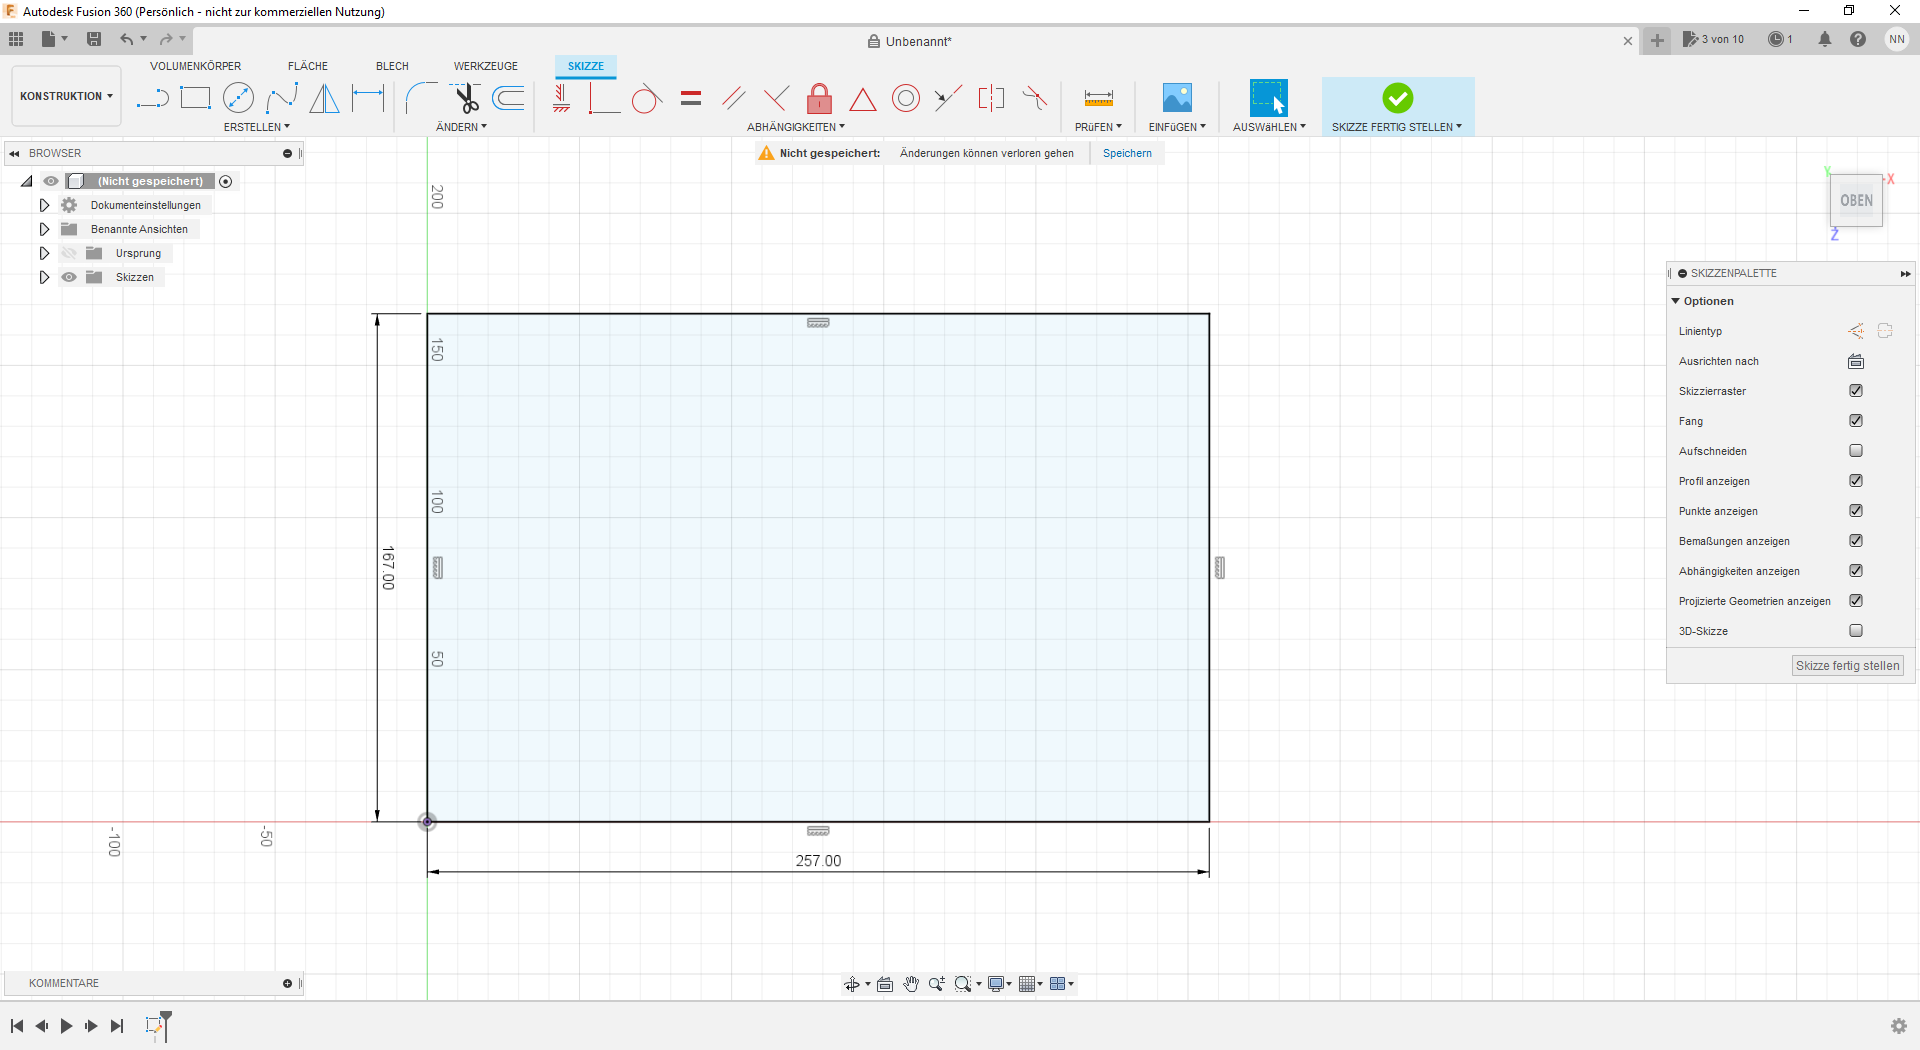
\includegraphics[width=1\textwidth]{img/konstruktion_gehaeuse_001.png}
		\caption[Zeichnen der Außenmaße]{Zeichnen der Außenmaße}
		\label{fig:design-case-01}
	\end{subfigure}
	\begin{subfigure}[b]{.5\linewidth}
		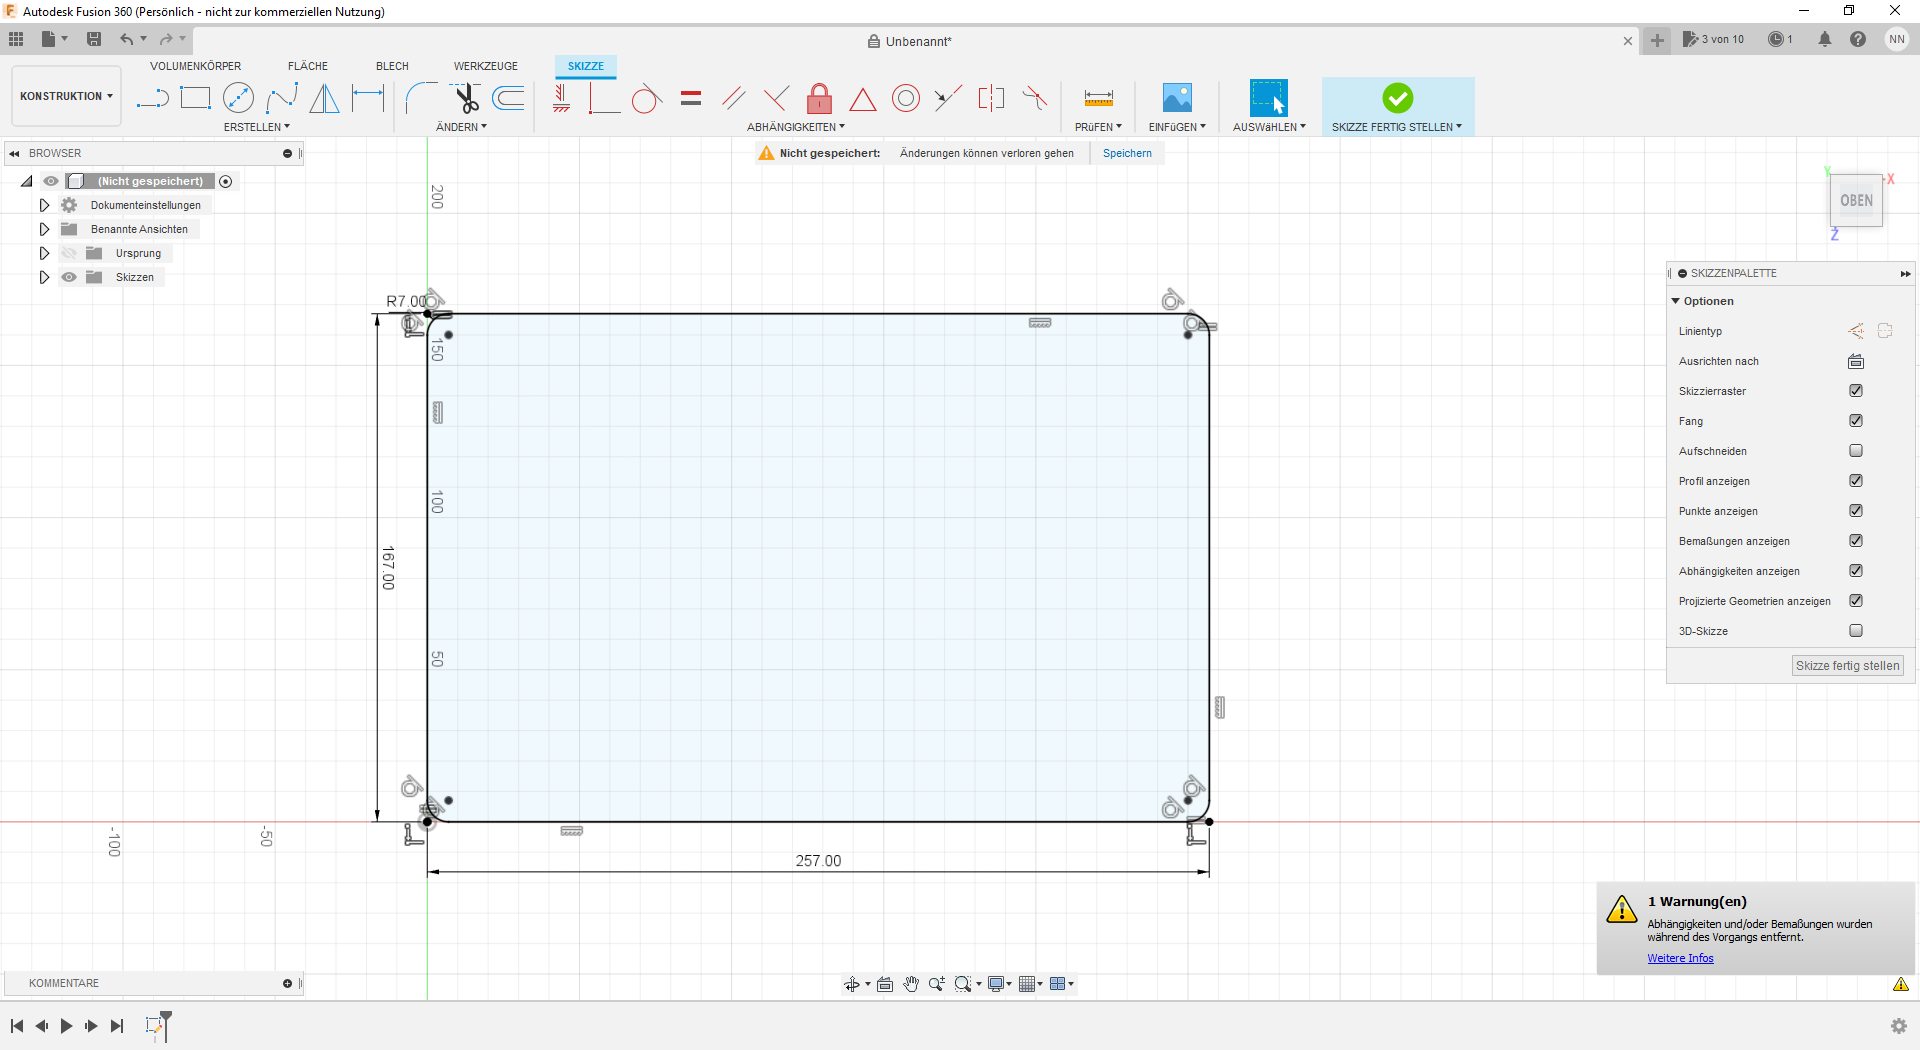
\includegraphics[width=1\textwidth]{img/konstruktion_gehaeuse_002.png}
		\caption[Abrunden der Ecken]{Abrunden der Ecken}
		\label{fig:design-case-02}
	\end{subfigure}
	\begin{subfigure}[b]{.5\linewidth}
		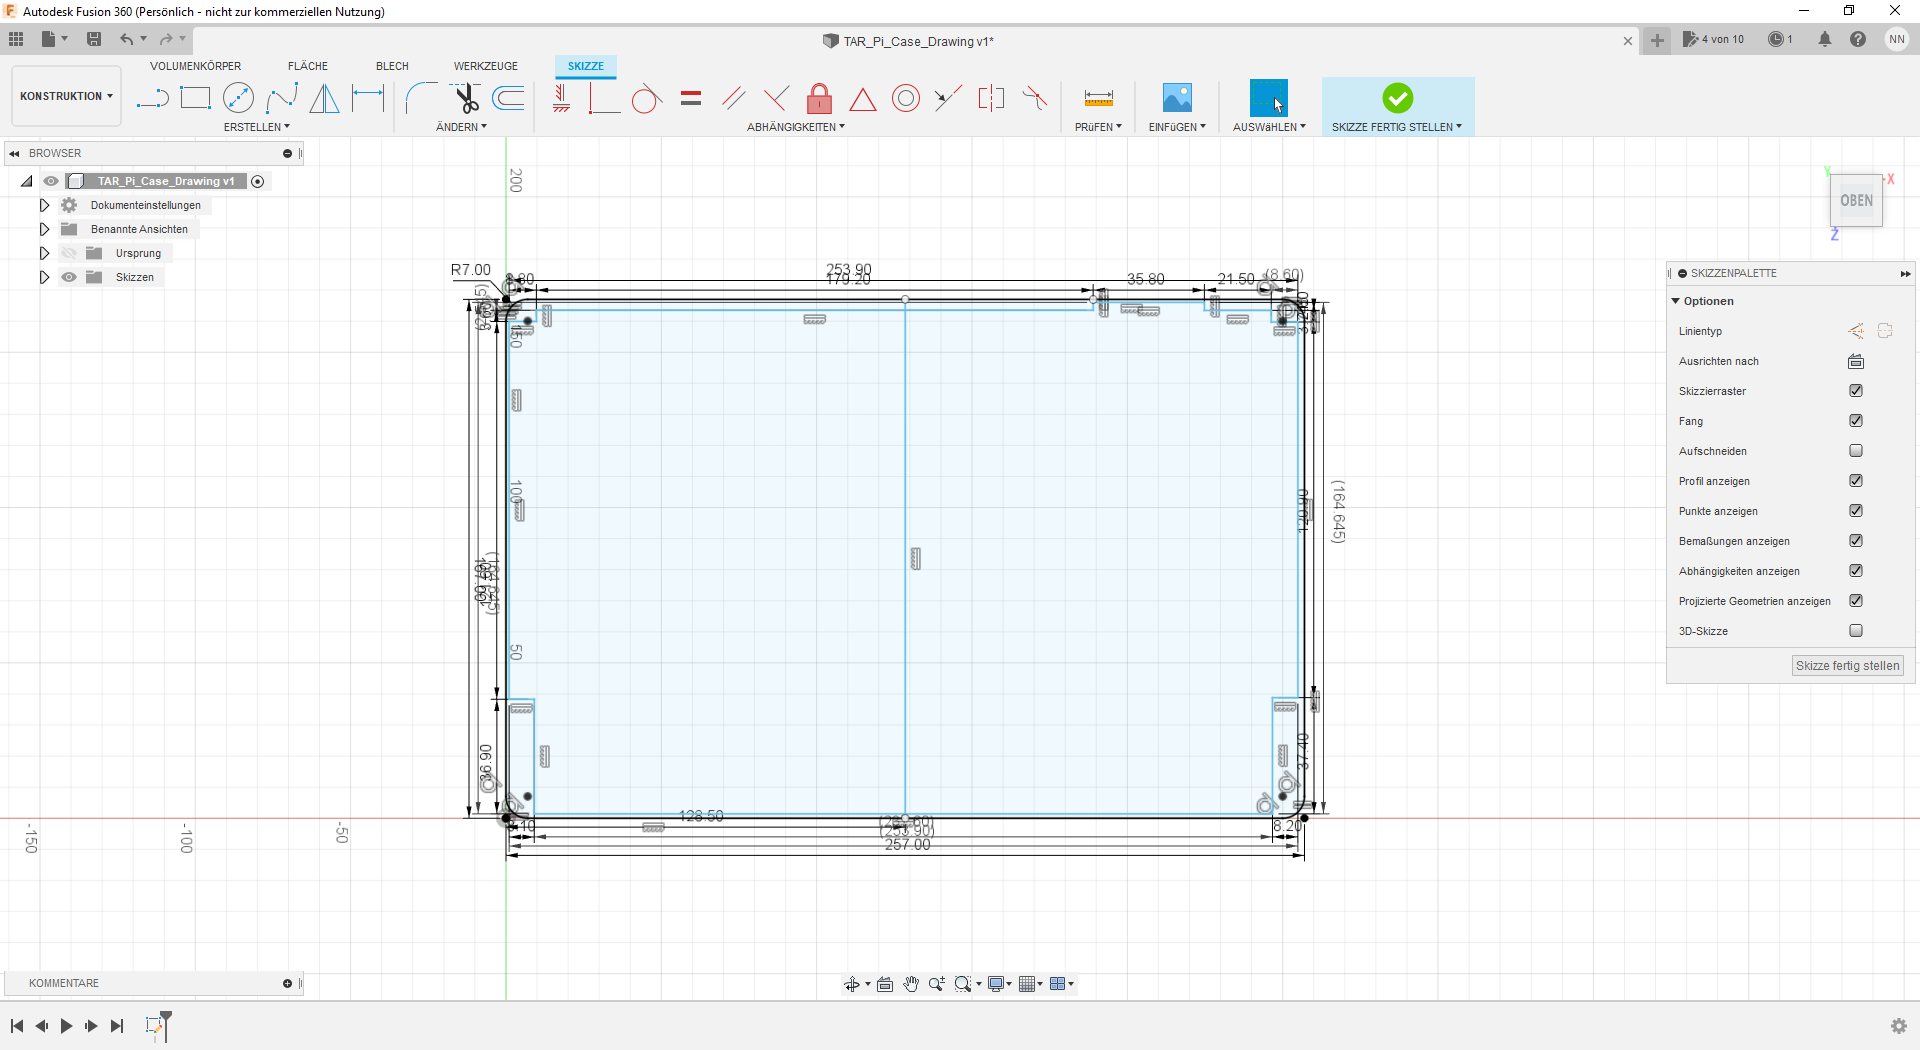
\includegraphics[width=1\textwidth]{img/konstruktion_gehaeuse_003.png}
		\caption[Zeichnen der Auflageflächen für das Gehäuse]{Zeichnen der Auflageflächen}
		\label{fig:design-case-03}
	\end{subfigure}
	\caption[Grundzeichnung als Basis des Modells]{Grundzeichnung als Basis des Modells}
	\label{fig:design-case-base}
\end{figure}\par
Die so entstandene Zeichnung (vgl. \ref{fig:design-case-03}) wurde dann in eine weitere Datei kopiert um als Grundlage für die beiden geteilten Seitenteile zu dienen. Von hier aus wurden die beiden Wand-Teile mehr oder weniger unabhängig voneinander entworfen.\par
\paragraph{Linkes Wandteil}
Beim linken Wandteil wurde der entsprechende Teil der Zeichnung um 2 mm entlang der Z-Achse extrudiert (vgl. \ref{fig:design-left-01}). Auf der erhöhten Seite wurde darauf hin eine weitere Zeichnung gelegt, die die Bleche an der Rückseite des Bildschirms überdecken sollte (vgl. \ref{fig:design-left-02}), die dann wie zuvor um 3 mm entlang der Z-Achse extrudiert wurde (vgl. \ref{fig:design-left-03}). Diese sollte dem Gehäuse genug Auflagefläche an dem Bildschirm bieten, um die Verklebung so stark wie möglich zu machen. Auf die nun entstandene erhöhte Seite wurde eine Zeichnung der ,,tatsächlichen'' Wandstärke von 3 mm erstellt (vgl. \ref{fig:design-left-04}). Diese wurde dann um 6 mm entlang der Z-Achse extrudiert, um für die Verbinder genügend Platz vor dem klobigen Blechbereich im unteren Teil des Bildschirms zu bieten (vgl. \ref{fig:design-left-05}). Auf die nun obenliegende Seite wurde die Zeichnung der Verbindungsstücke gelegt (vgl. \ref{fig:design-left-06}) und um 19 mm entlang der Z-Achse extrudiert (vgl. \ref{fig:design-left-07}) und im Kreismittelpunkt der Zeichnungen eine Bohrung für M3-Gewinde gesetzt (vgl. \ref{fig:design-left-08}). Auf die nun  entstandene Oberfläche wurde die Zeichnung für die Deckelverbindung gesetzt (vgl. \ref{fig:design-left-09}), um 25 mm entlang der Z-Achse extrudiert (vgl. \ref{fig:design-left-10}) und ebenfalls mit Bohrungen für M3-Gewinde versehen (vgl. \ref{fig:design-left-11}).\\
%beschreibungstext links
\begin{figure}[h!tb]
	\begin{subfigure}[t]{.3\linewidth}
		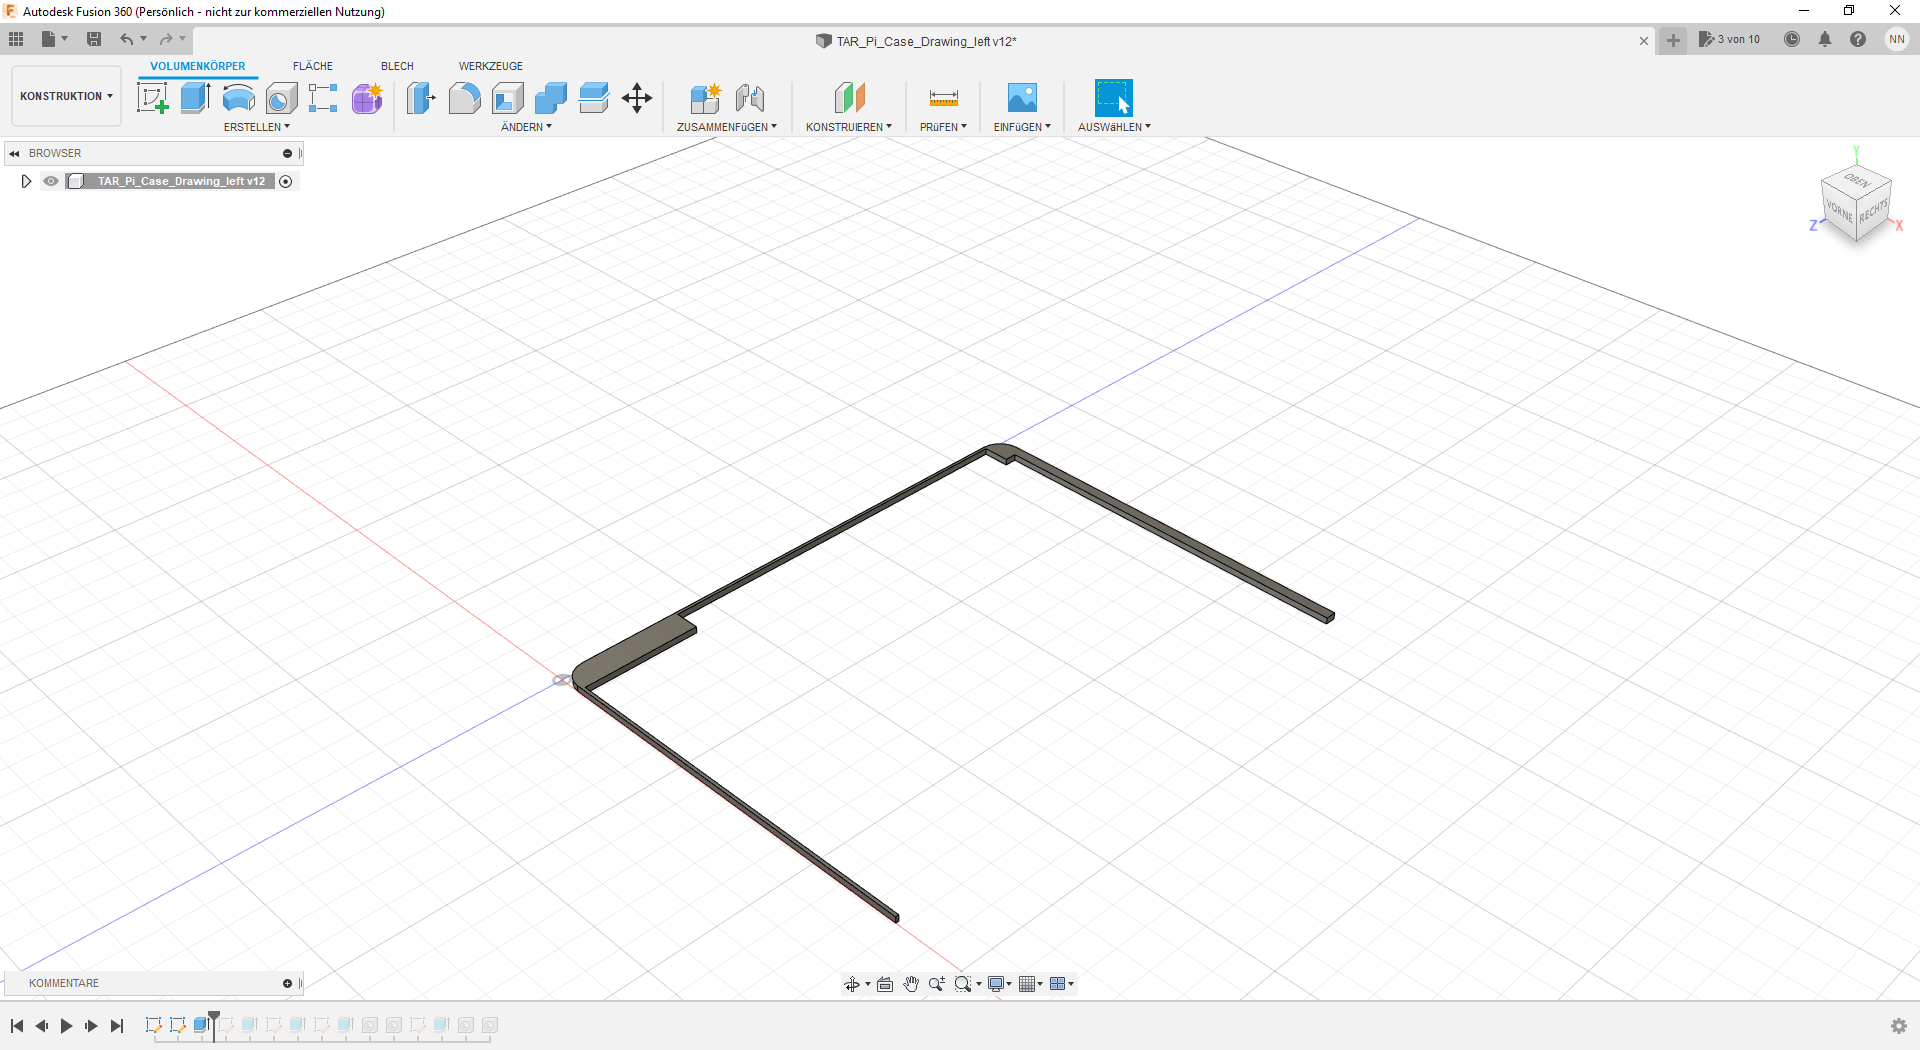
\includegraphics[width=\linewidth]{img/konstruktion_gehaeuse_links_001.png}
		\caption[Extrusion der Grundzeichnung]{Extrusion der Grundzeichnung}
		\label{fig:design-left-01}
	\end{subfigure}
	\begin{subfigure}[t]{.3\linewidth}
		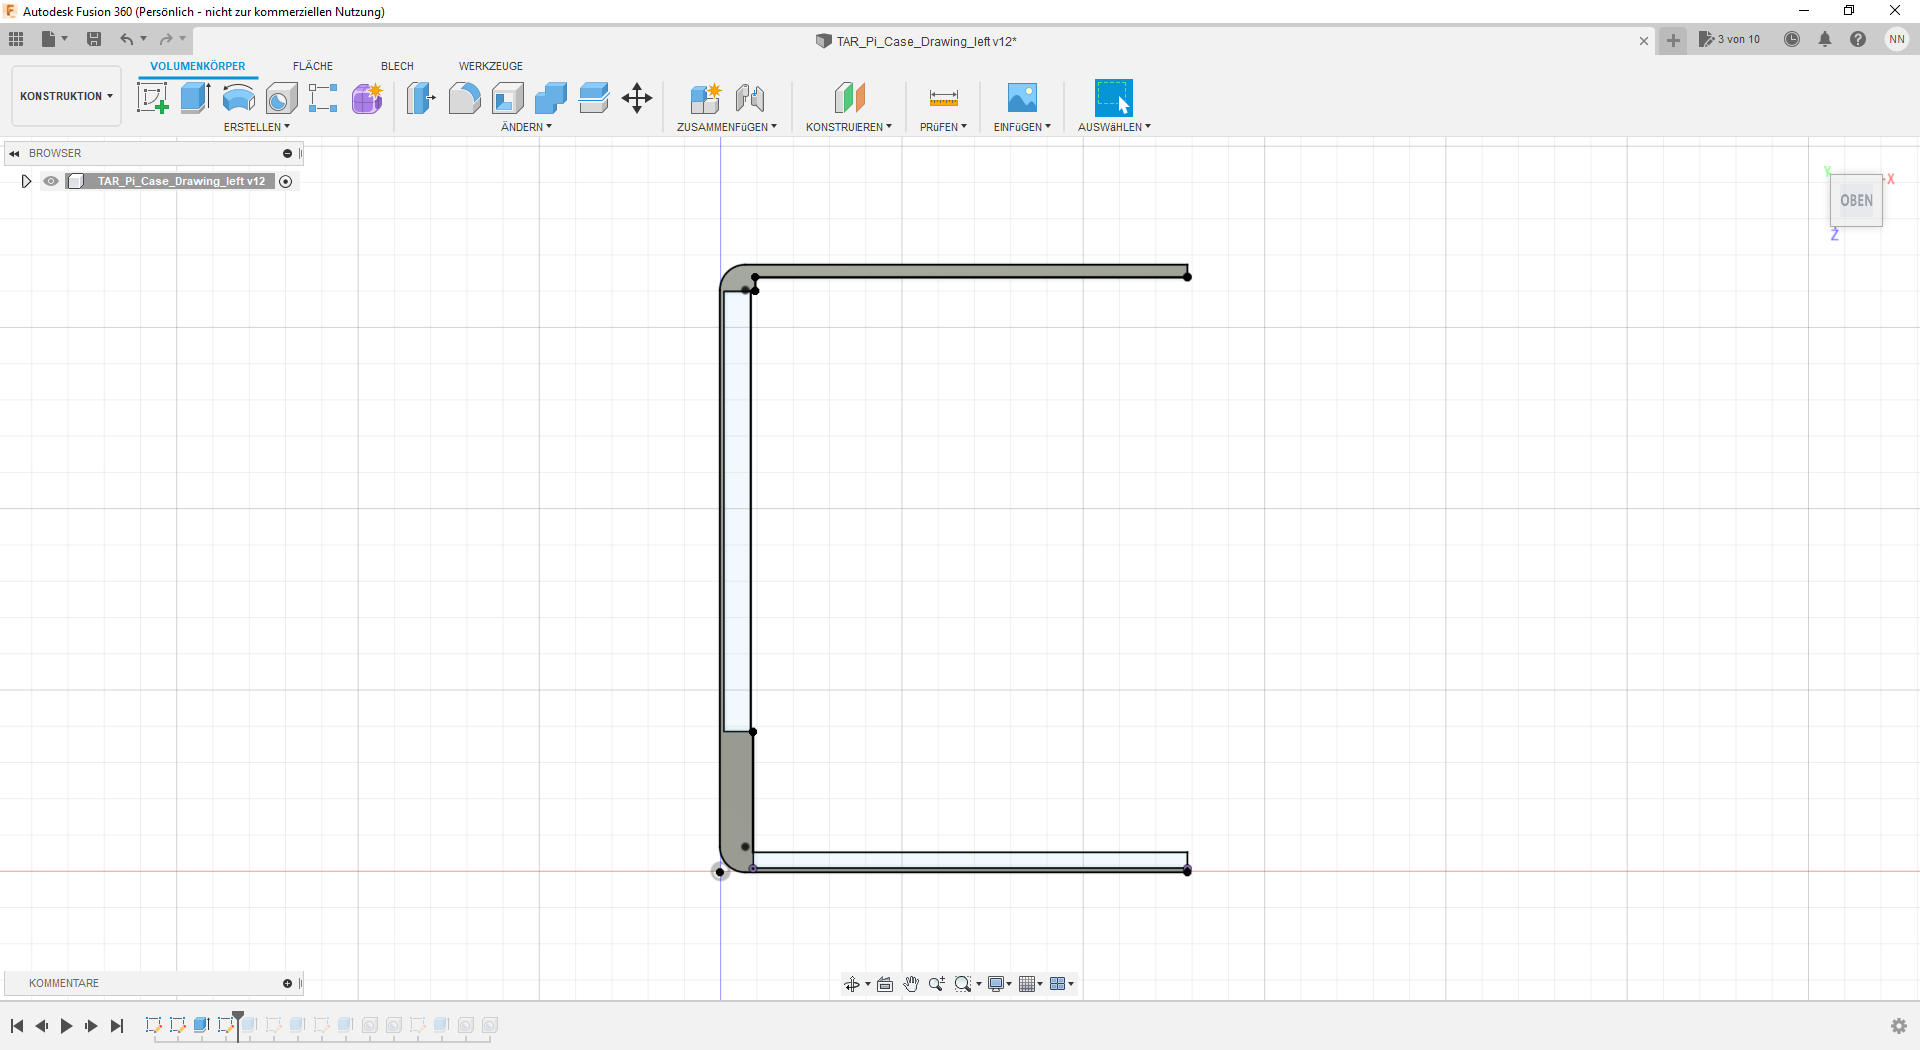
\includegraphics[width=\linewidth]{img/konstruktion_gehaeuse_links_002.png}
		\caption[Erstellung der Folgezeichnung um Blech]{Erstellung der Folgezeichnung um Blech}
		\label{fig:design-left-02}
	\end{subfigure}
	\begin{subfigure}[t]{.3\linewidth}
		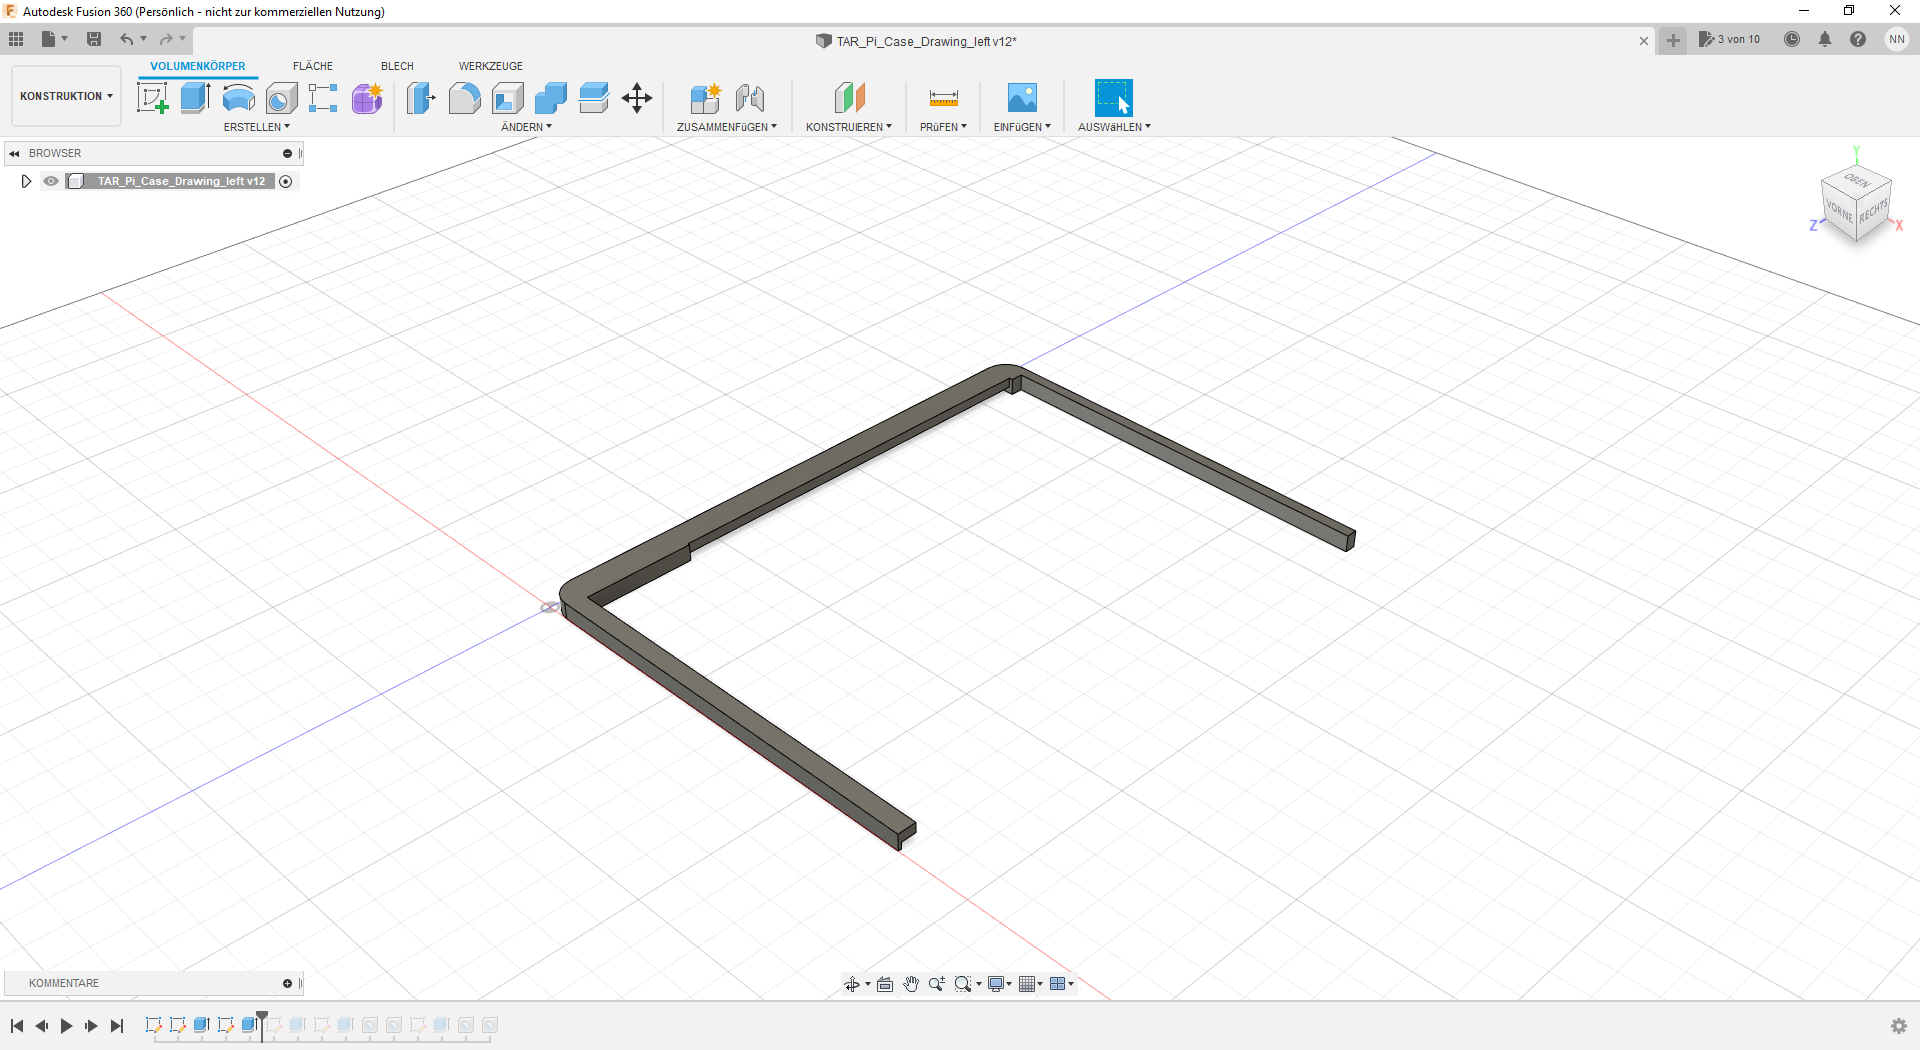
\includegraphics[width=\linewidth]{img/konstruktion_gehaeuse_links_003.png}
		\caption[Extrusion der neuen Zeichnung]{Extrusion der neuen Zeichnung}
		\label{fig:design-left-03}
	\end{subfigure}
	\begin{subfigure}[t]{.3\linewidth}
		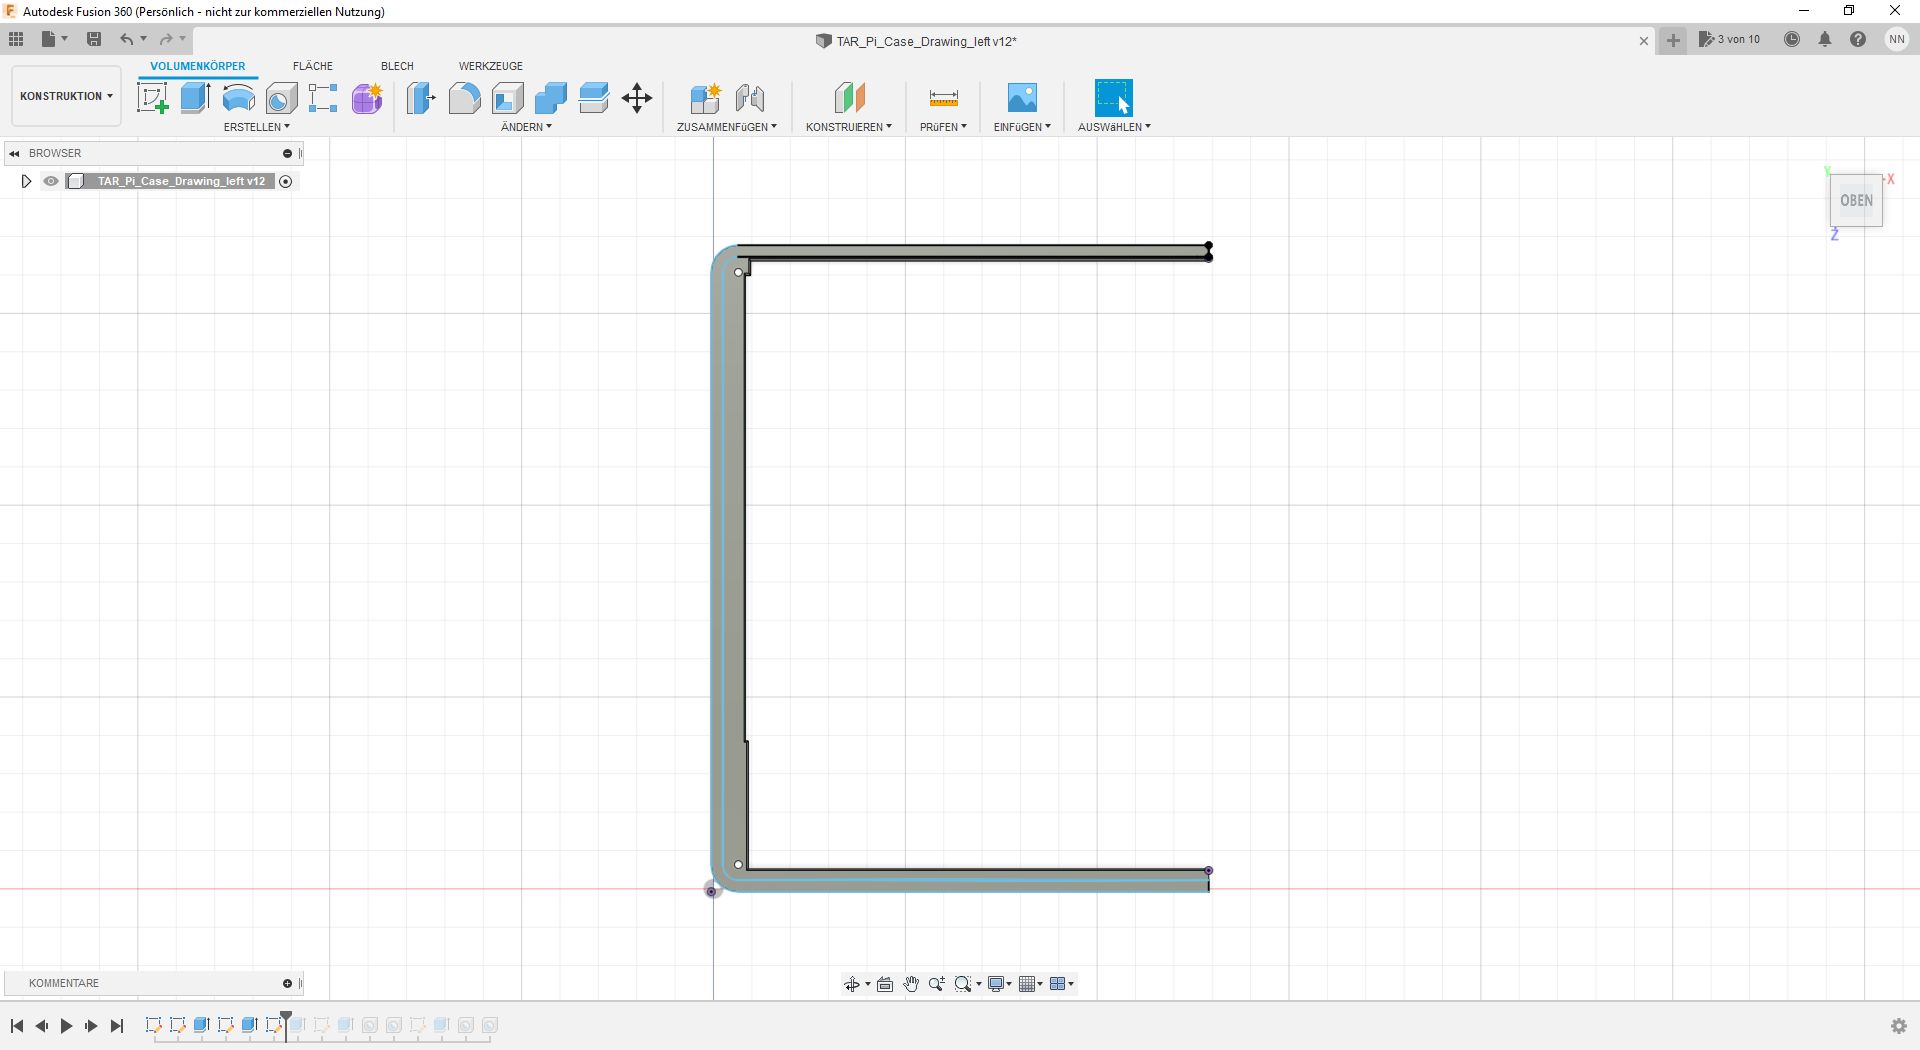
\includegraphics[width=\linewidth]{img/konstruktion_gehaeuse_links_004.png}
		\caption[Zeichnung der Hauptwandstärke]{Zeichnung der Hauptwandstärke}
		\label{fig:design-left-04}
	\end{subfigure}
	\begin{subfigure}[t]{.3\linewidth}
		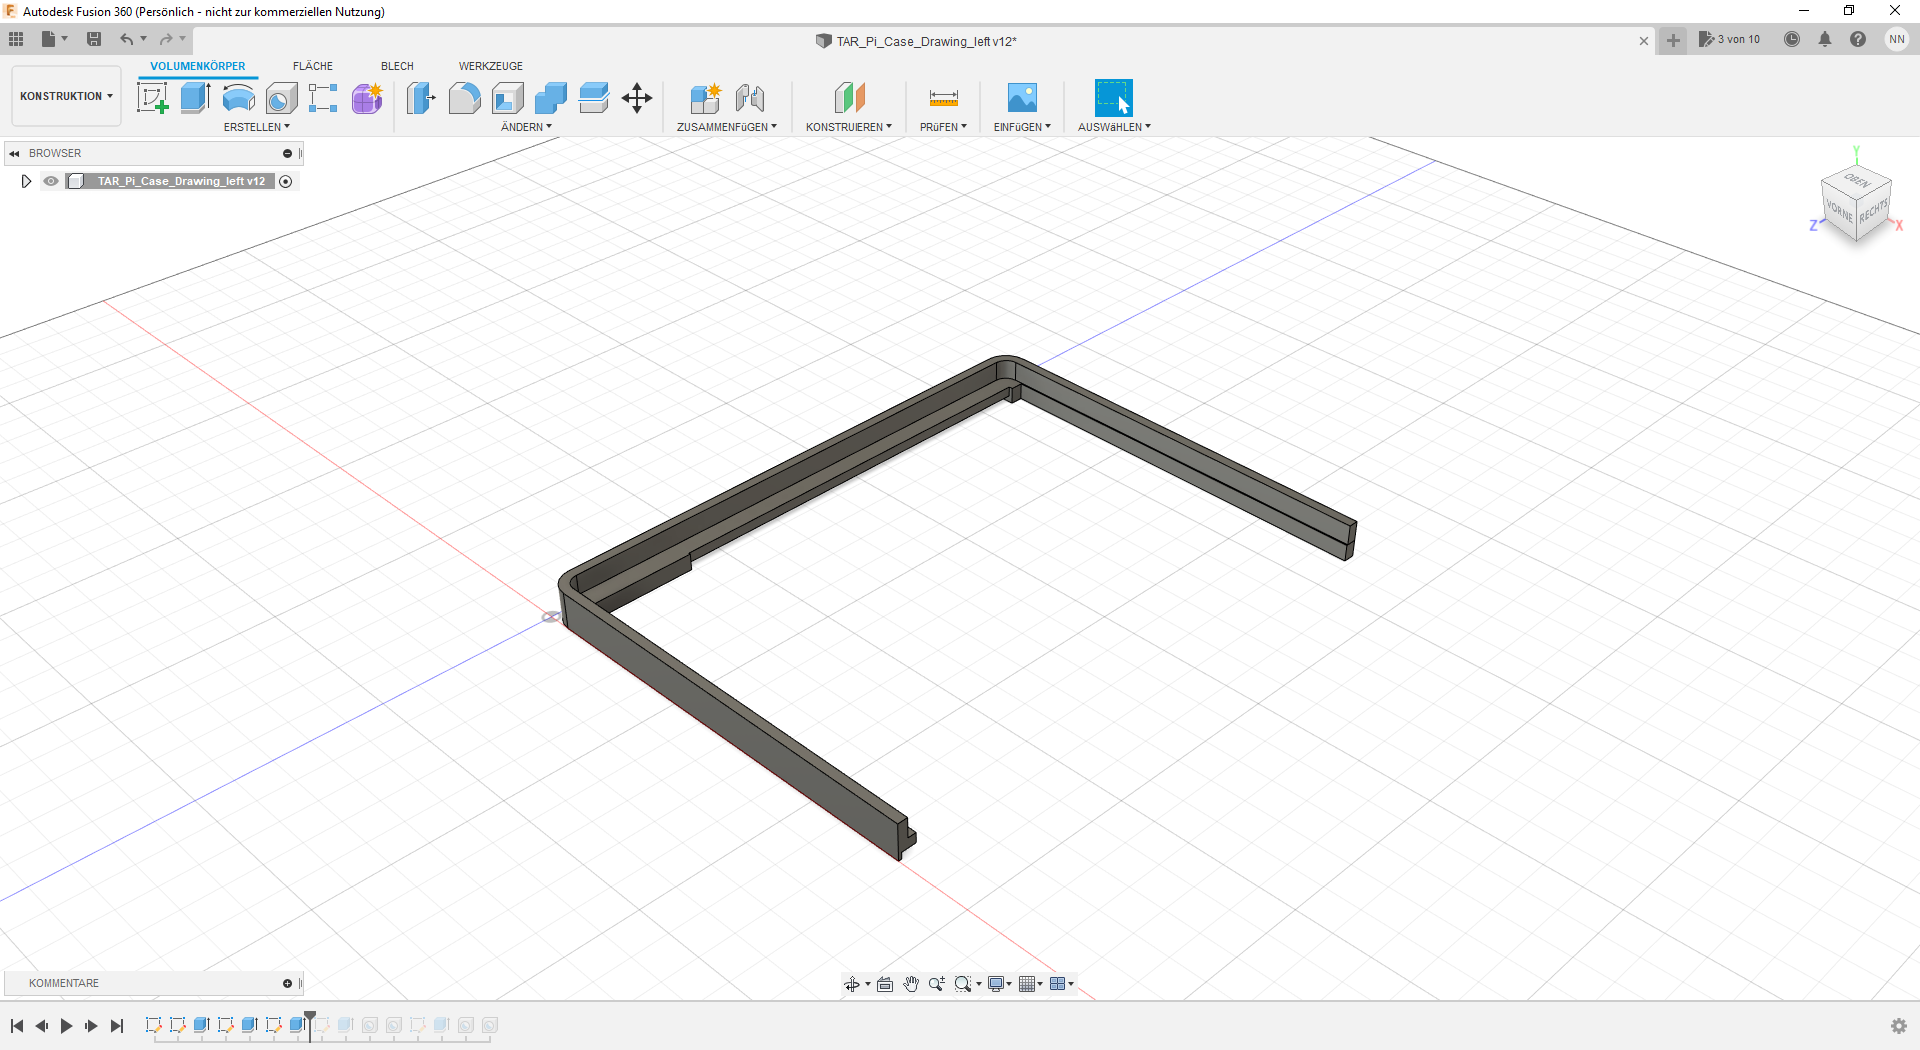
\includegraphics[width=\linewidth]{img/konstruktion_gehaeuse_links_005.png}
		\caption[Extrusion der Hauptwand]{Extrusion der Hauptwand}
		\label{fig:design-left-05}
	\end{subfigure}
	\begin{subfigure}[t]{.3\linewidth}
		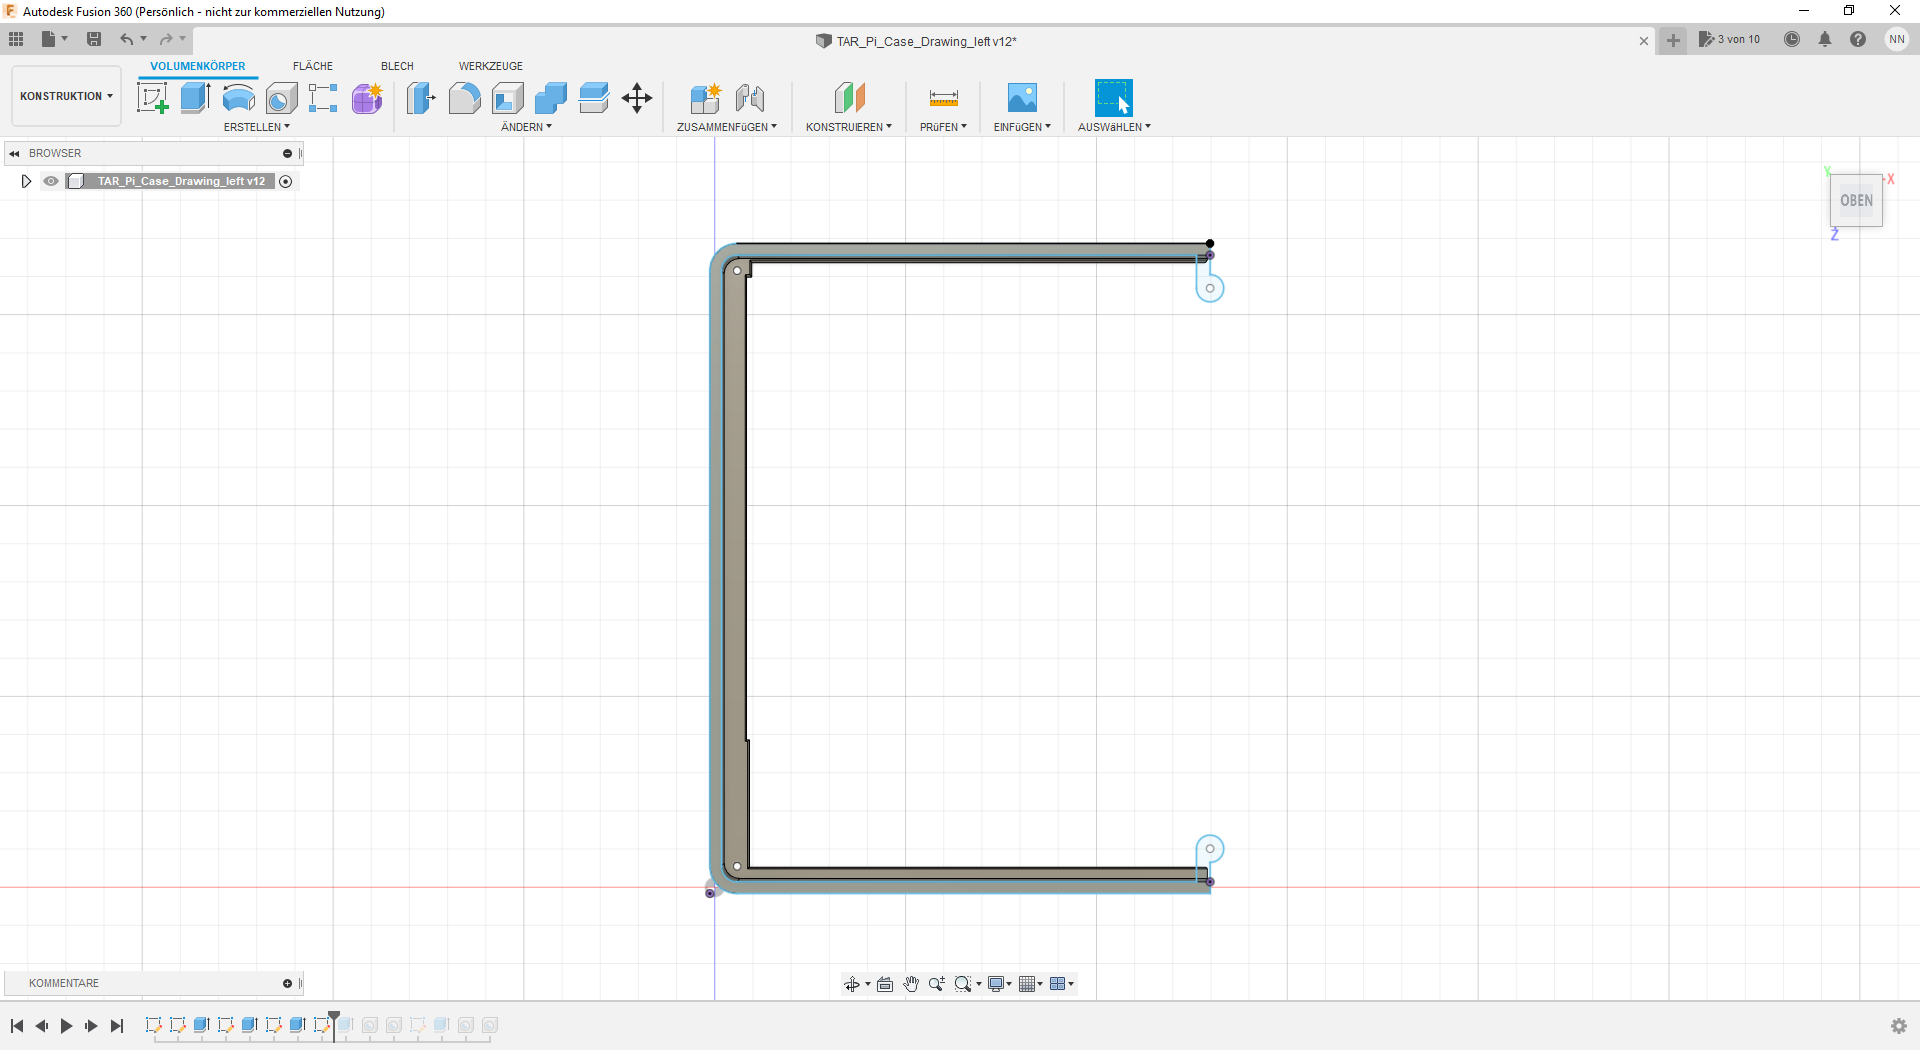
\includegraphics[width=\linewidth]{img/konstruktion_gehaeuse_links_006.png}
		\caption[Zeichnung der Verbindungsstücke]{Zeichnung der Verbindungsstücke}
		\label{fig:design-left-06}
	\end{subfigure}
	\begin{subfigure}[t]{.3\linewidth}
		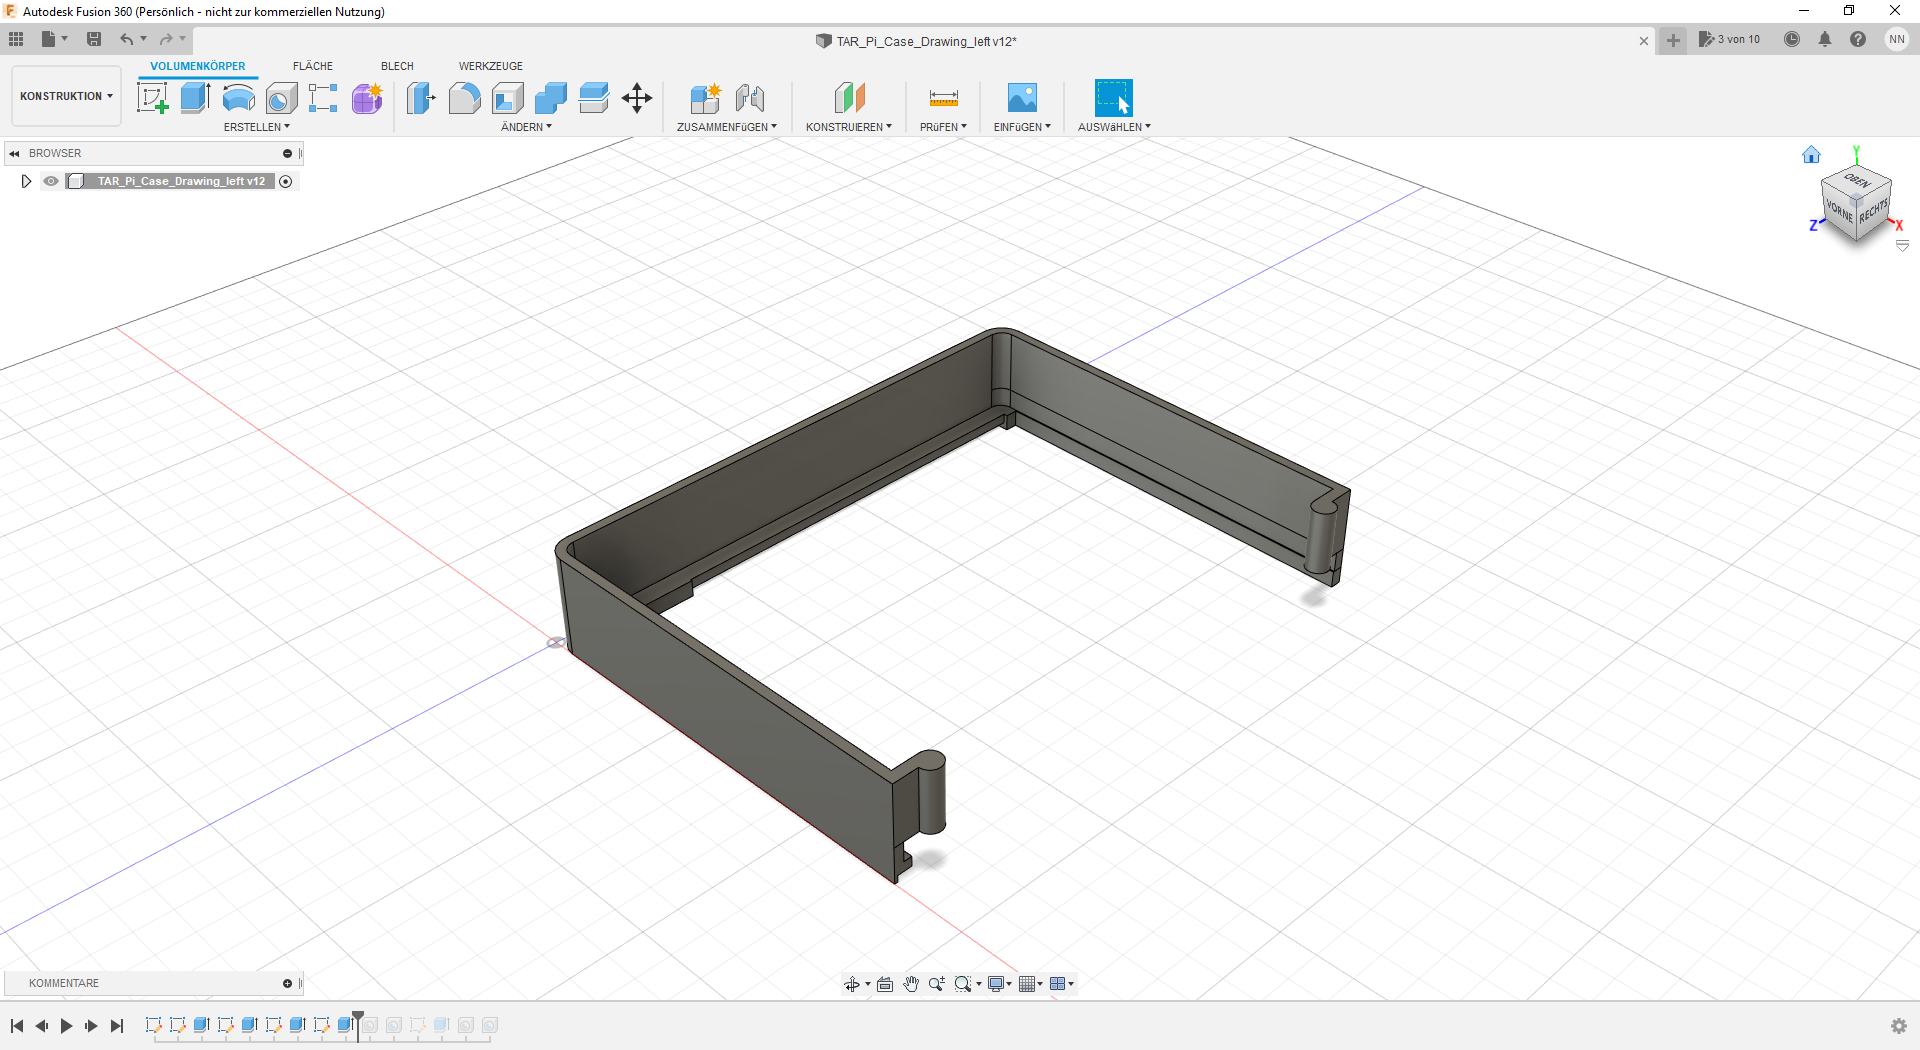
\includegraphics[width=\linewidth]{img/konstruktion_gehaeuse_links_007.png}
		\caption[Extrusion der Hauptwand mit Verbindungsstücken]{Extrusion der Hauptwand mit Verbindungsstücken}
		\label{fig:design-left-07}
	\end{subfigure}
	\begin{subfigure}[t]{.3\linewidth}
		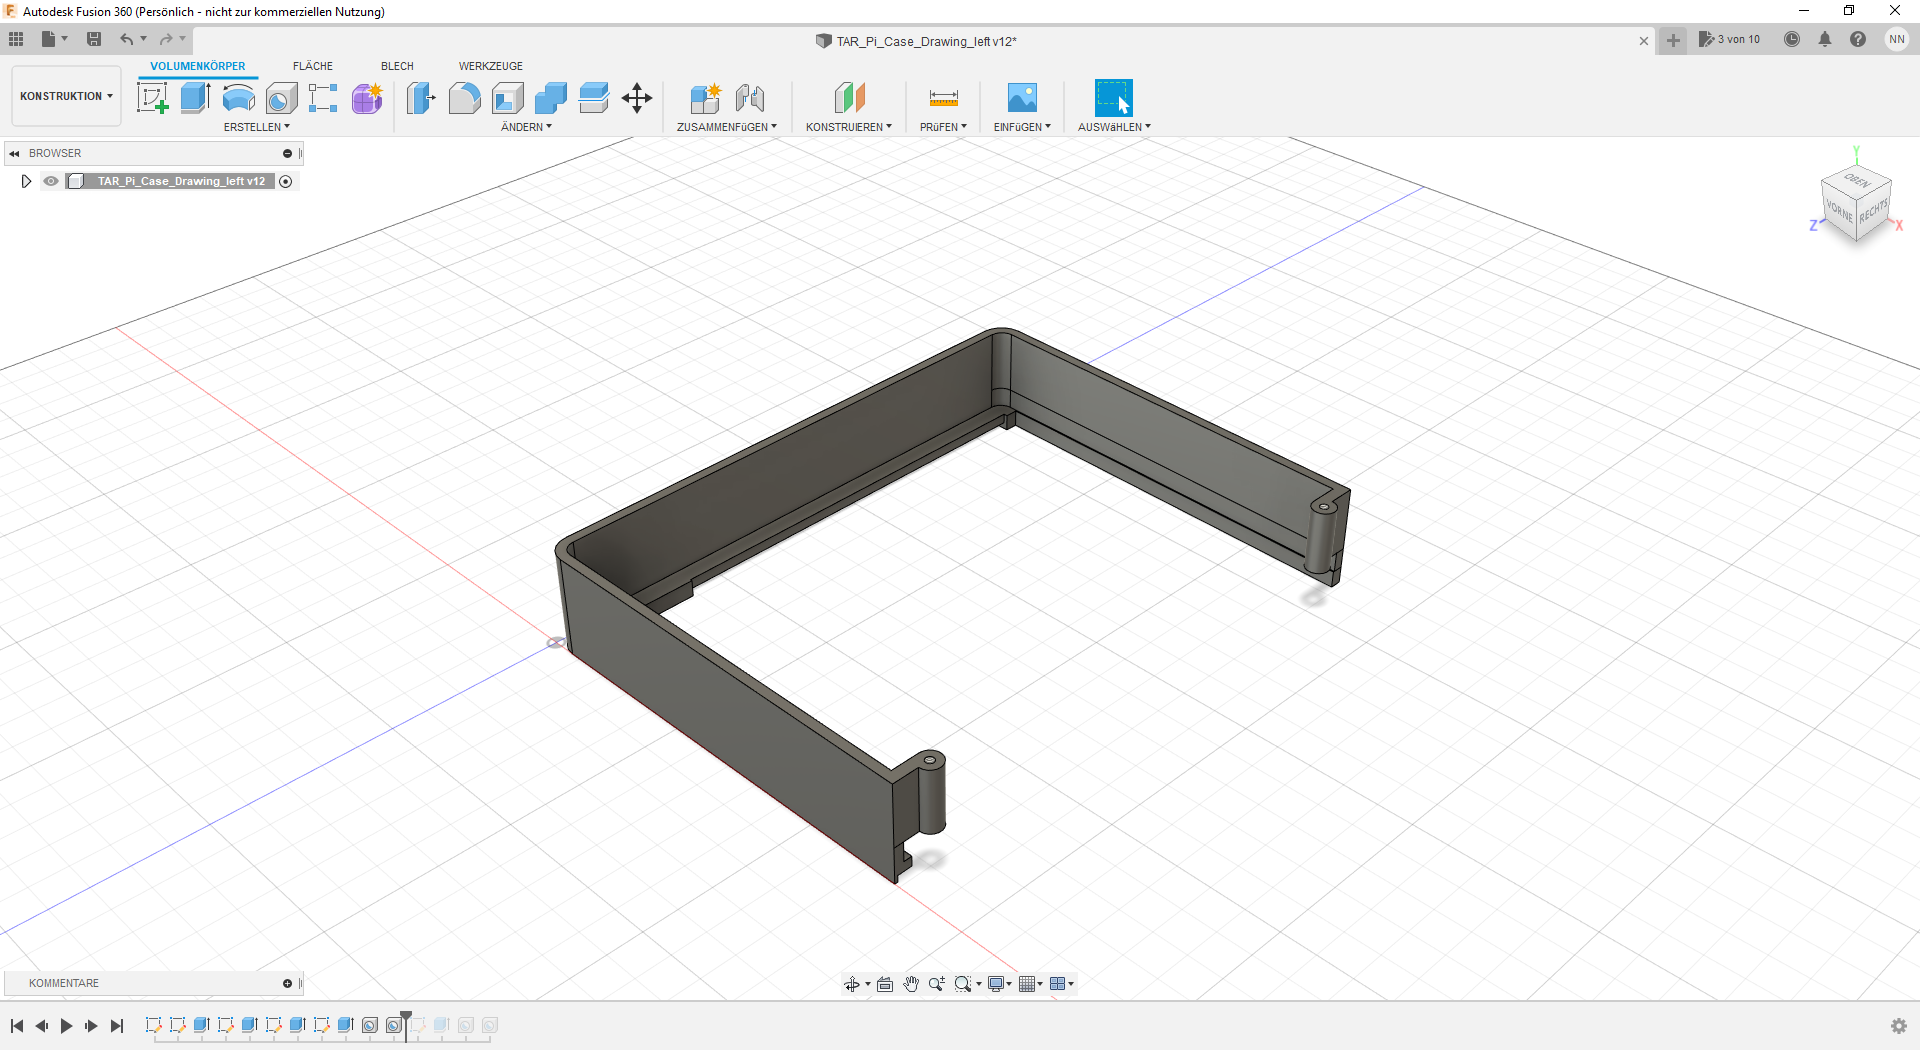
\includegraphics[width=\linewidth]{img/konstruktion_gehaeuse_links_008.png}
		\caption[Bohrung für Schrauben]{Bohrung für Schrauben}
		\label{fig:design-left-08}
	\end{subfigure}
	\begin{subfigure}[t]{.3\linewidth}
		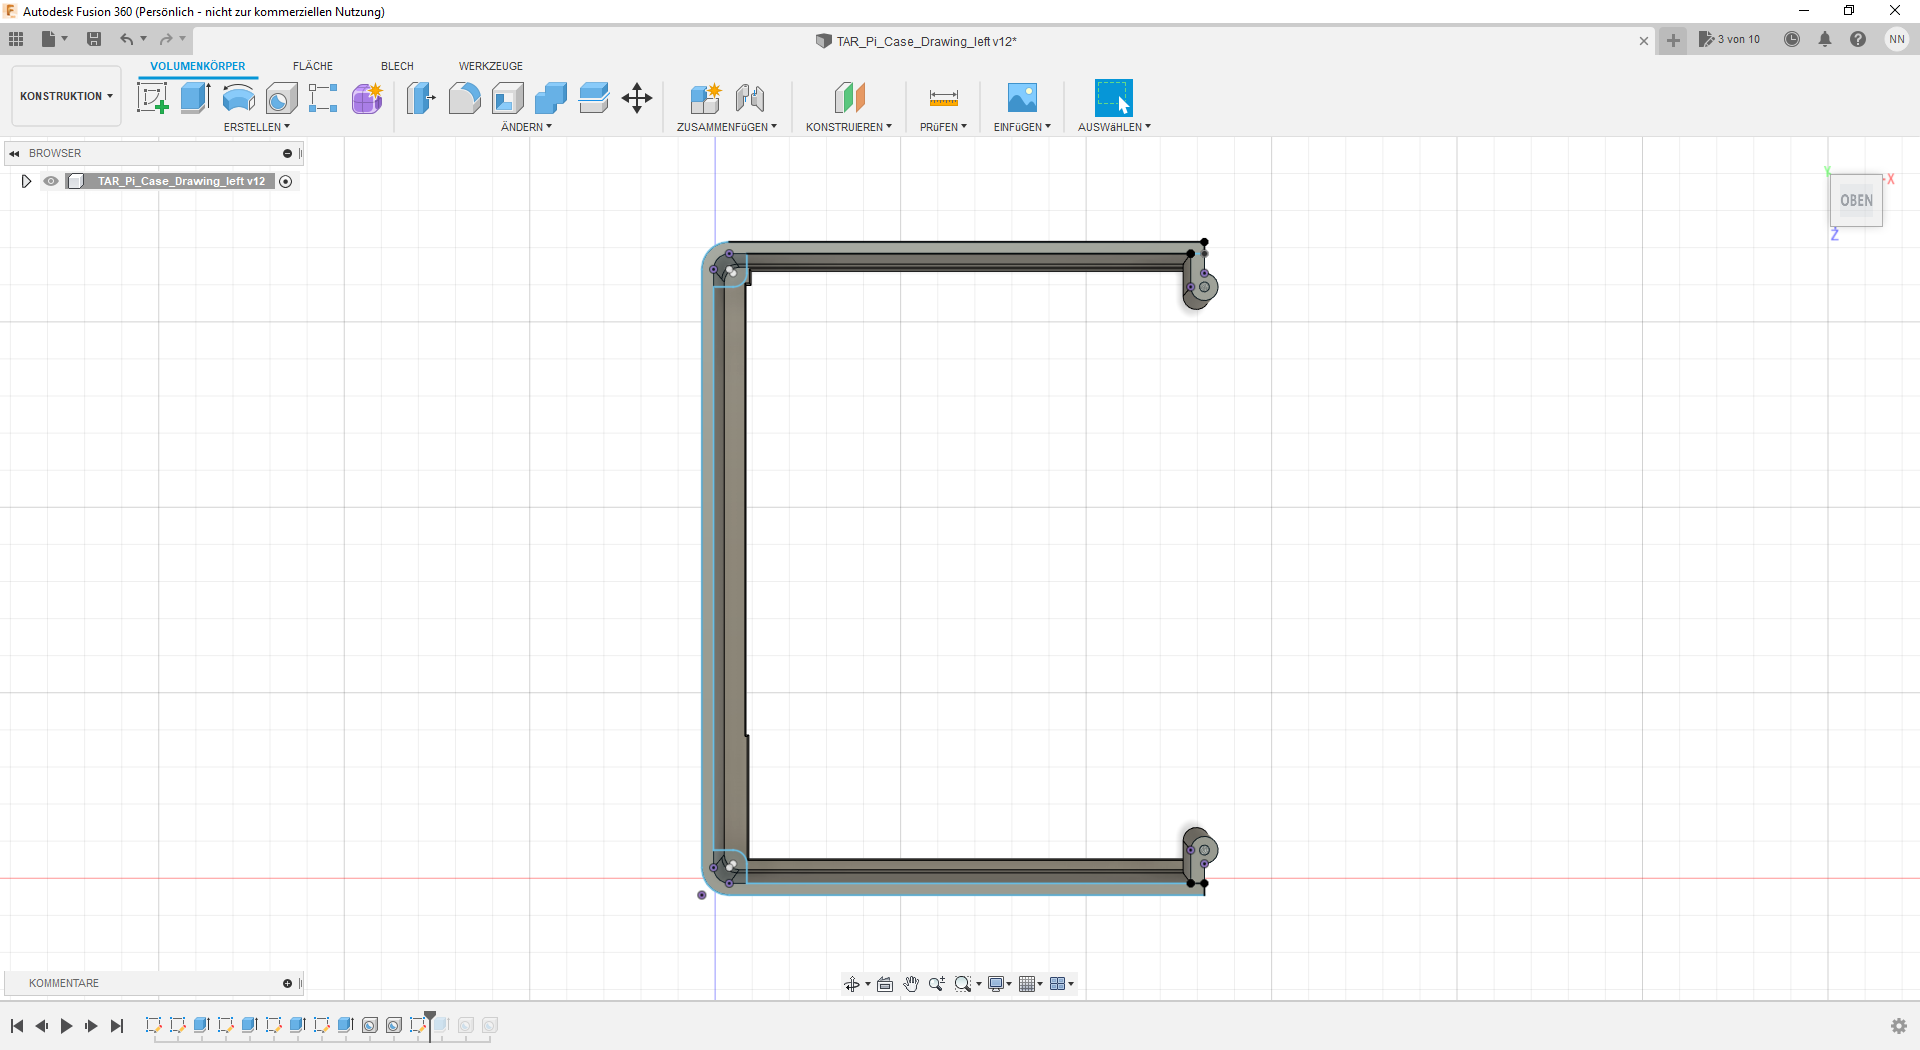
\includegraphics[width=\linewidth]{img/konstruktion_gehaeuse_links_009.png}
		\caption[Zeichnung der Deckelverbindung]{Zeichnung der Deckelverbindung}
		\label{fig:design-left-09}
	\end{subfigure}
	\begin{subfigure}[t]{.3\linewidth}
		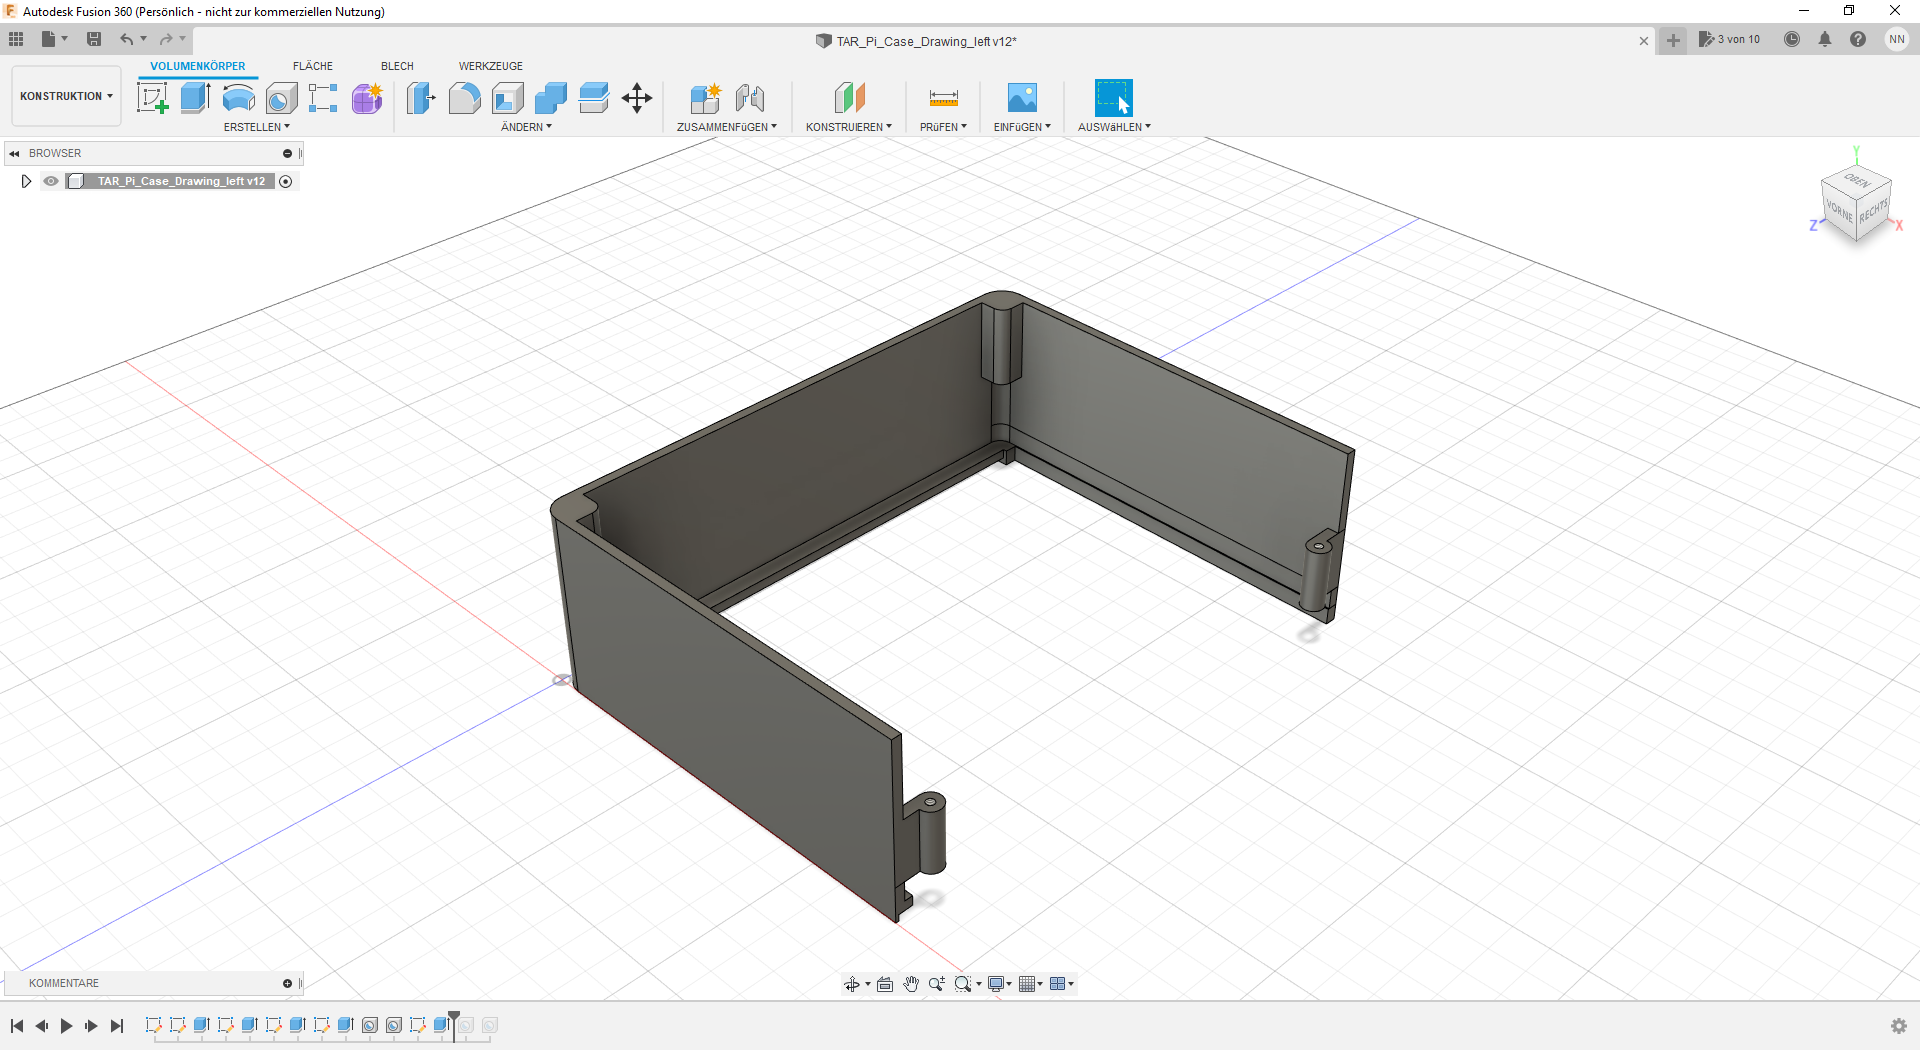
\includegraphics[width=\linewidth]{img/konstruktion_gehaeuse_links_010.png}
		\caption[Extrusion der Hauptwand mit Deckelverbindung]{Extrusion der Hauptwand mit Deckelverbindung}
		\label{fig:design-left-10}
	\end{subfigure}
	\begin{subfigure}[t]{.3\linewidth}
		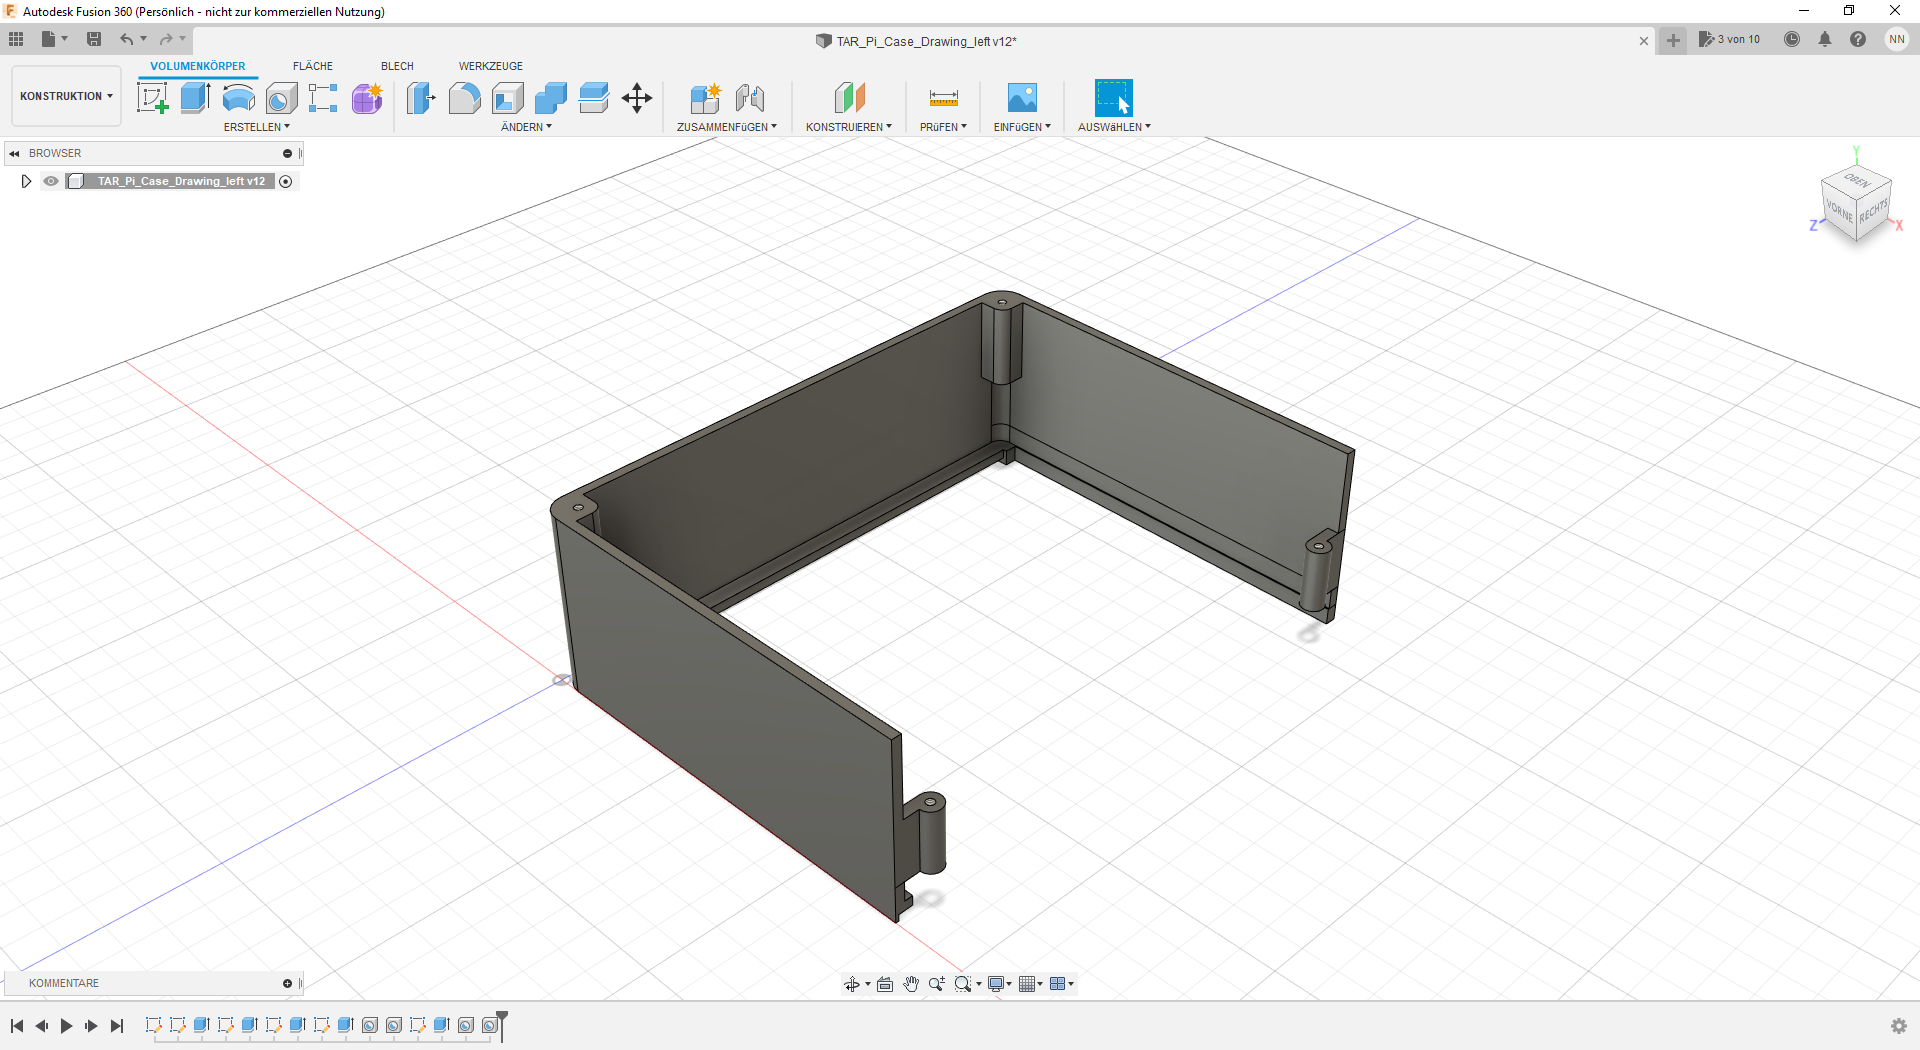
\includegraphics[width=\linewidth]{img/konstruktion_gehaeuse_links_011.png}
		\caption[Bohrungen der Deckelverbindung]{Bohrungen der Deckelverbindung}
		\label{fig:design-left-11}
	\end{subfigure}
	\caption[Entwurf des linken Wandteils]{Entwurf des linken Wandteils}
	\label{fig:design-left}
\end{figure}\par
\paragraph{Rechtes Wandteil}
Beim rechten Teil des Gehäuses war die Vorgehensweise weitestgehend die selbe wie beim linken Gehäuseteil (vgl. \ref{fig:design-right-01} - \ref{fig:design-right-08} mit \ref{fig:design-left}). Der Unterschied zwischen beiden Teilen, abgesehen von den Verbindungsstücken und der Aussparung für das Flachkabel des Bildschirms, waren die Aussparungen für Lüfter, Antenne, Netzwerkanschluss und Strombuchse. Für den Lüfter und die Antenne wurde auf der ,,Oberseite'' des Gehäuses eine Zeichnung aufgelegt (vgl. \ref{fig:design-right-09}), die dann ins Negative extruiert wurde, was die gezeichnete Fläche aus dem Körper löscht (vgl. \ref{fig:design-right-10}). Auf ähnliche Weise wurde die Aussparung für eine RJ45-Verlängerung und eine 5,5 mm DC-Buchse gesetzt. Zuerst wurde die Zeichnung für die Aussparung auf die Seite gelegt (vgl. \ref{fig:design-right-11}), die dann ebenfalls ins Negative extruiert wurde (vgl. \ref{fig:design-right-12}). Um für die Befestigung der 5,5 mm DC-Buchse eine Unterlage im Gehäuse zu haben, wurde der Grundriss eines Rechtecks auf die Innenseite des Gehäusebodens gelegt (vgl. \ref{fig:design-right-13}) und extruiert (vgl. \ref{fig:design-right-14}), um die Möglichkeit zu bieten, die Buchse im Gehäuse zu verkleben. Damit die Buchse nicht zu tief im Gehäuse steckt, wurde eine Zeichnung eines konzentrischen Kreises auf die bereits vorhandene Aussparung auf die Innenseite gelegt  (vgl. \ref{fig:design-right-15}) und dann um einige Millimeter ins Negative extruiert, um die Aussparung zu generieren (vgl. \ref{fig:design-right}).\\
\begin{figure}[h!tb]
	\begin{subfigure}[t]{.3\linewidth}
		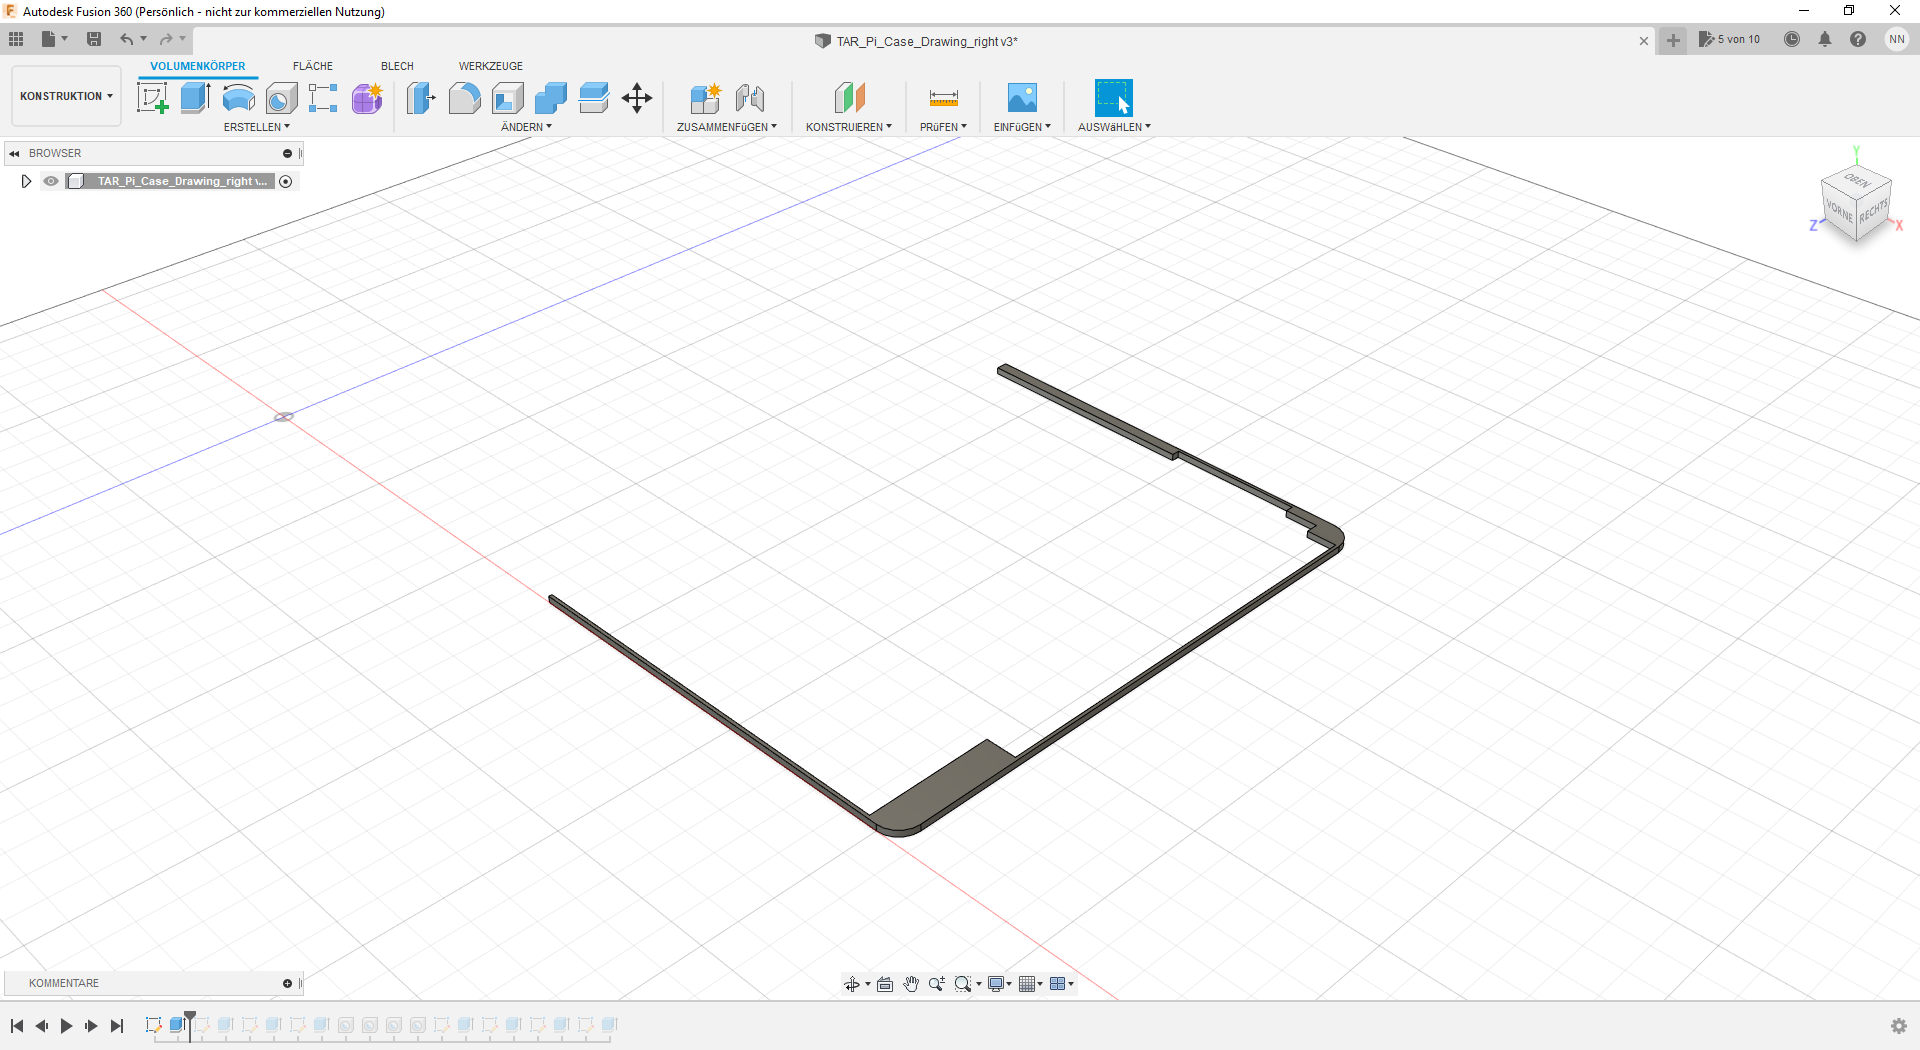
\includegraphics[width=\linewidth]{img/konstruktion_gehaeuse_rechts_001.png}
		\caption[]{}
		\label{fig:design-right-01}
	\end{subfigure}
	\begin{subfigure}[t]{.3\linewidth}
		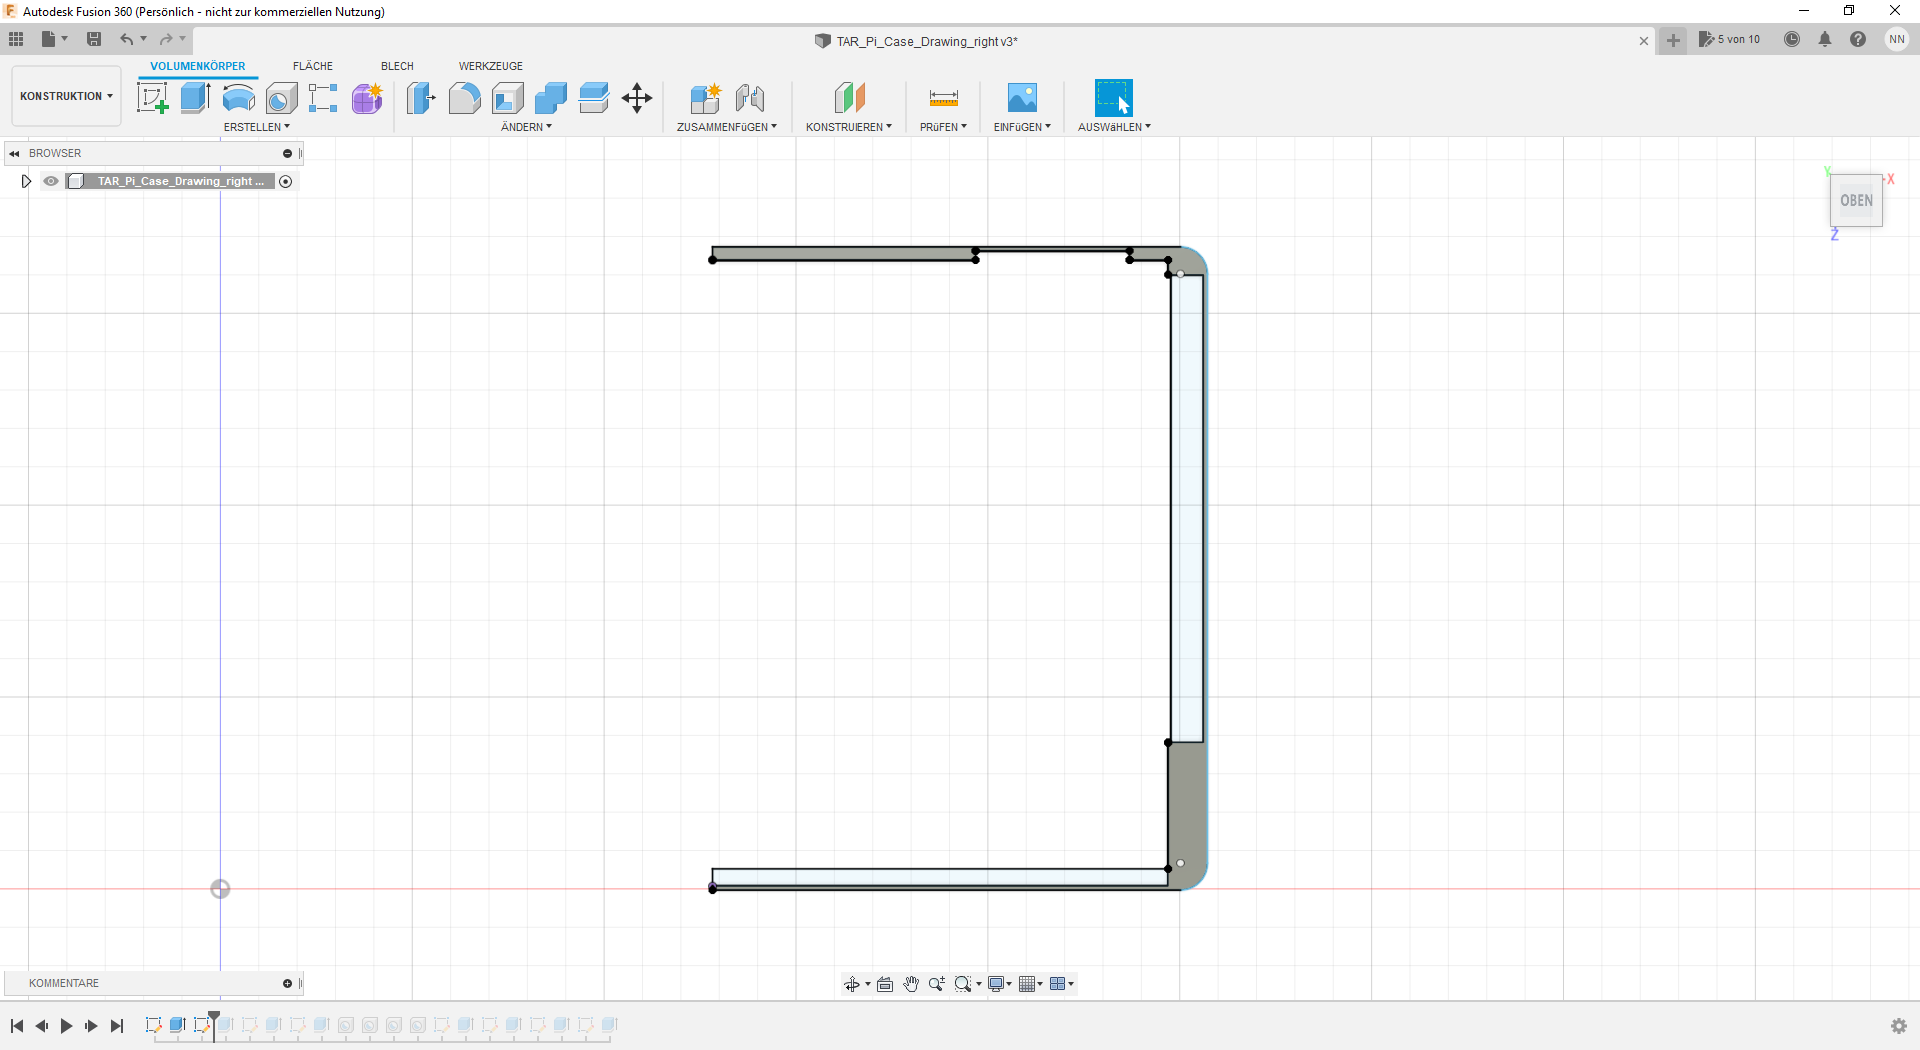
\includegraphics[width=\linewidth]{img/konstruktion_gehaeuse_rechts_002.png}
		\caption[]{}
		\label{fig:design-right-02}
	\end{subfigure}
	\begin{subfigure}[t]{.3\linewidth}
		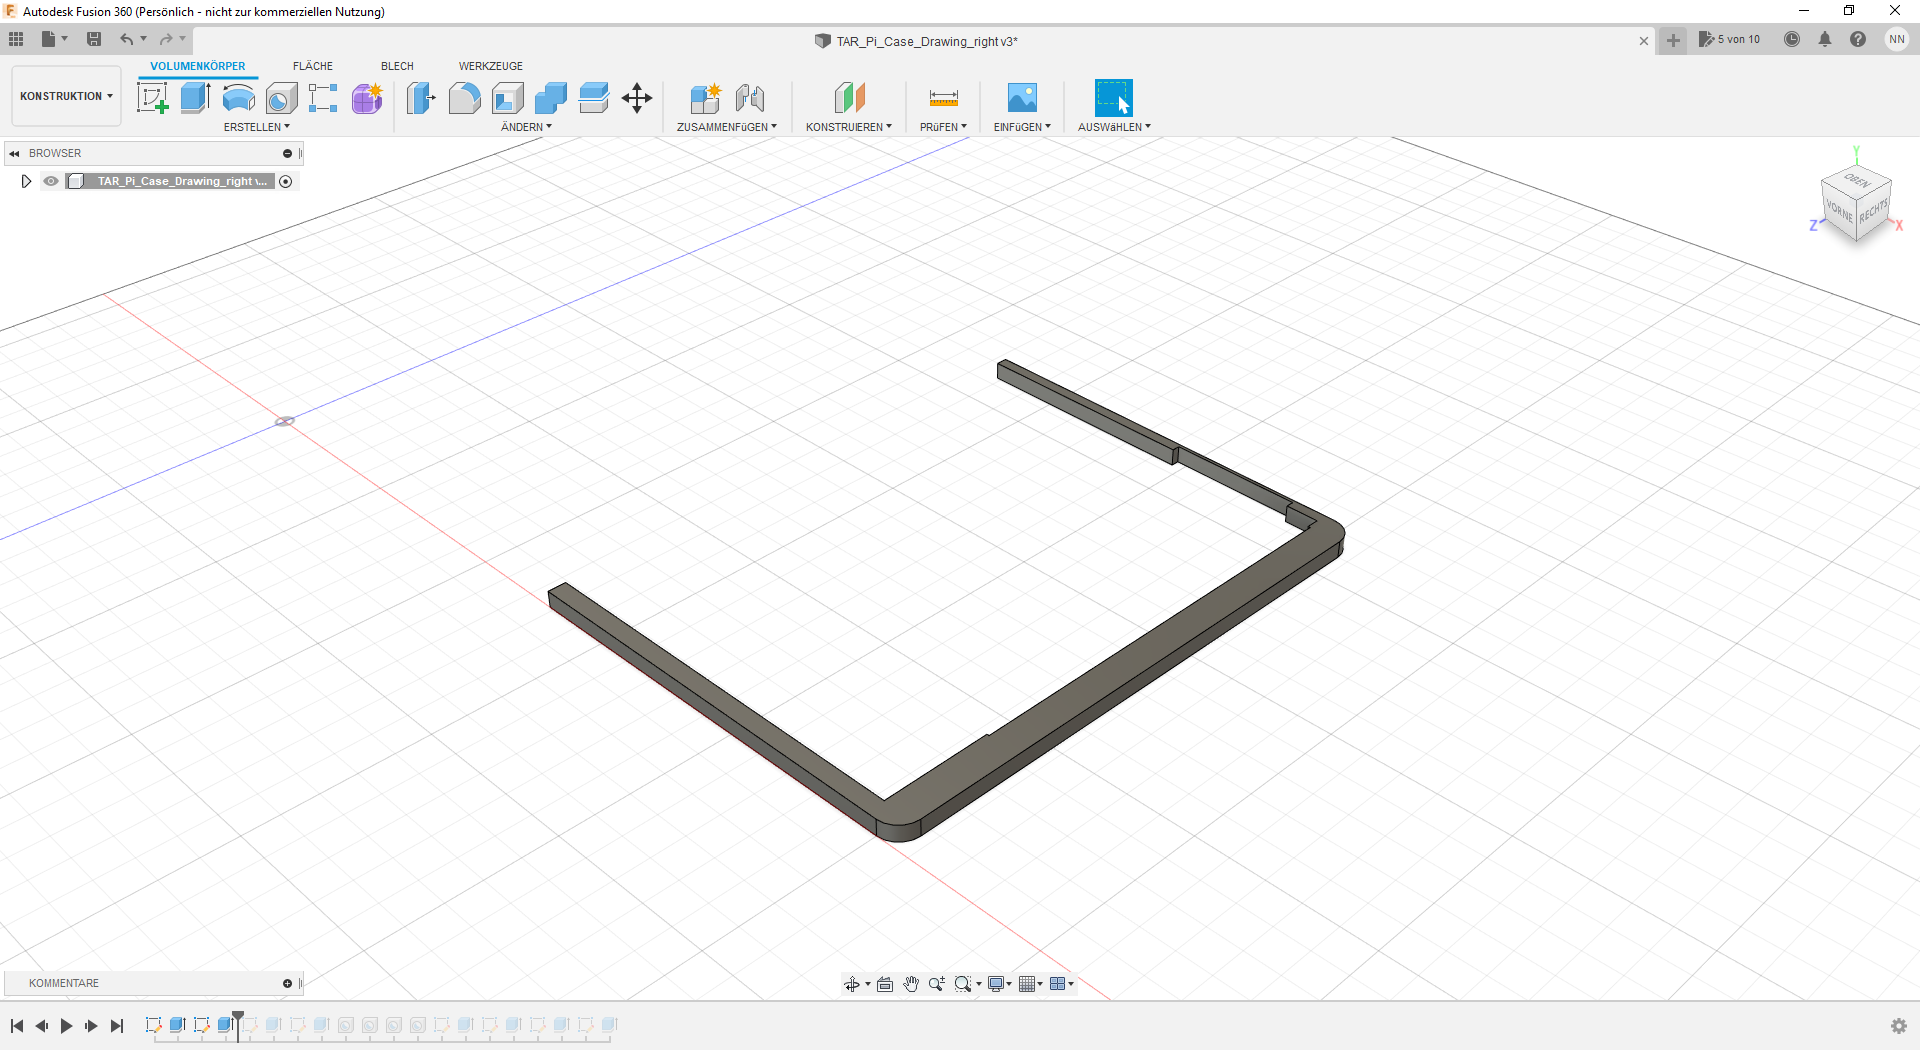
\includegraphics[width=\linewidth]{img/konstruktion_gehaeuse_rechts_003.png}
		\caption[]{}
		\label{fig:design-right-03}
	\end{subfigure}
	\begin{subfigure}[t]{.3\linewidth}
		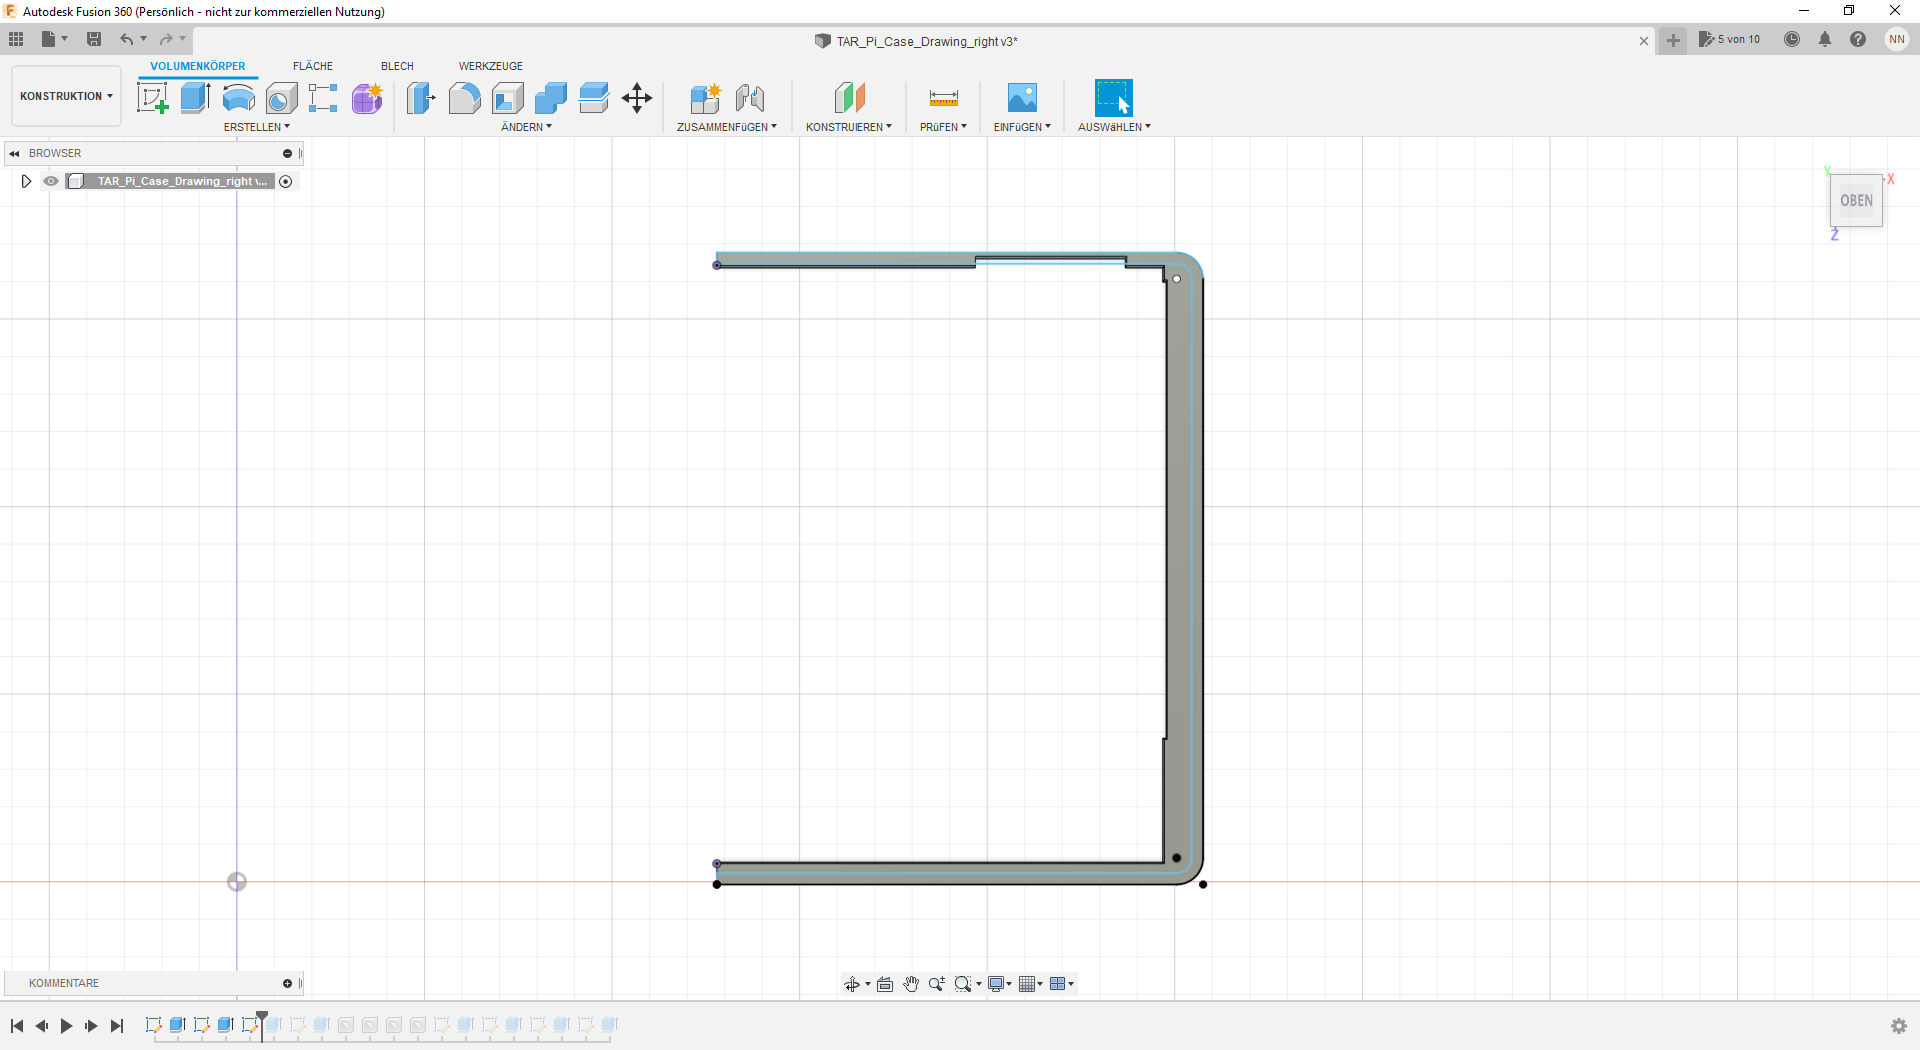
\includegraphics[width=\linewidth]{img/konstruktion_gehaeuse_rechts_004.png}
		\caption[]{}
		\label{fig:design-right-04}
	\end{subfigure}
	\begin{subfigure}[t]{.3\linewidth}
		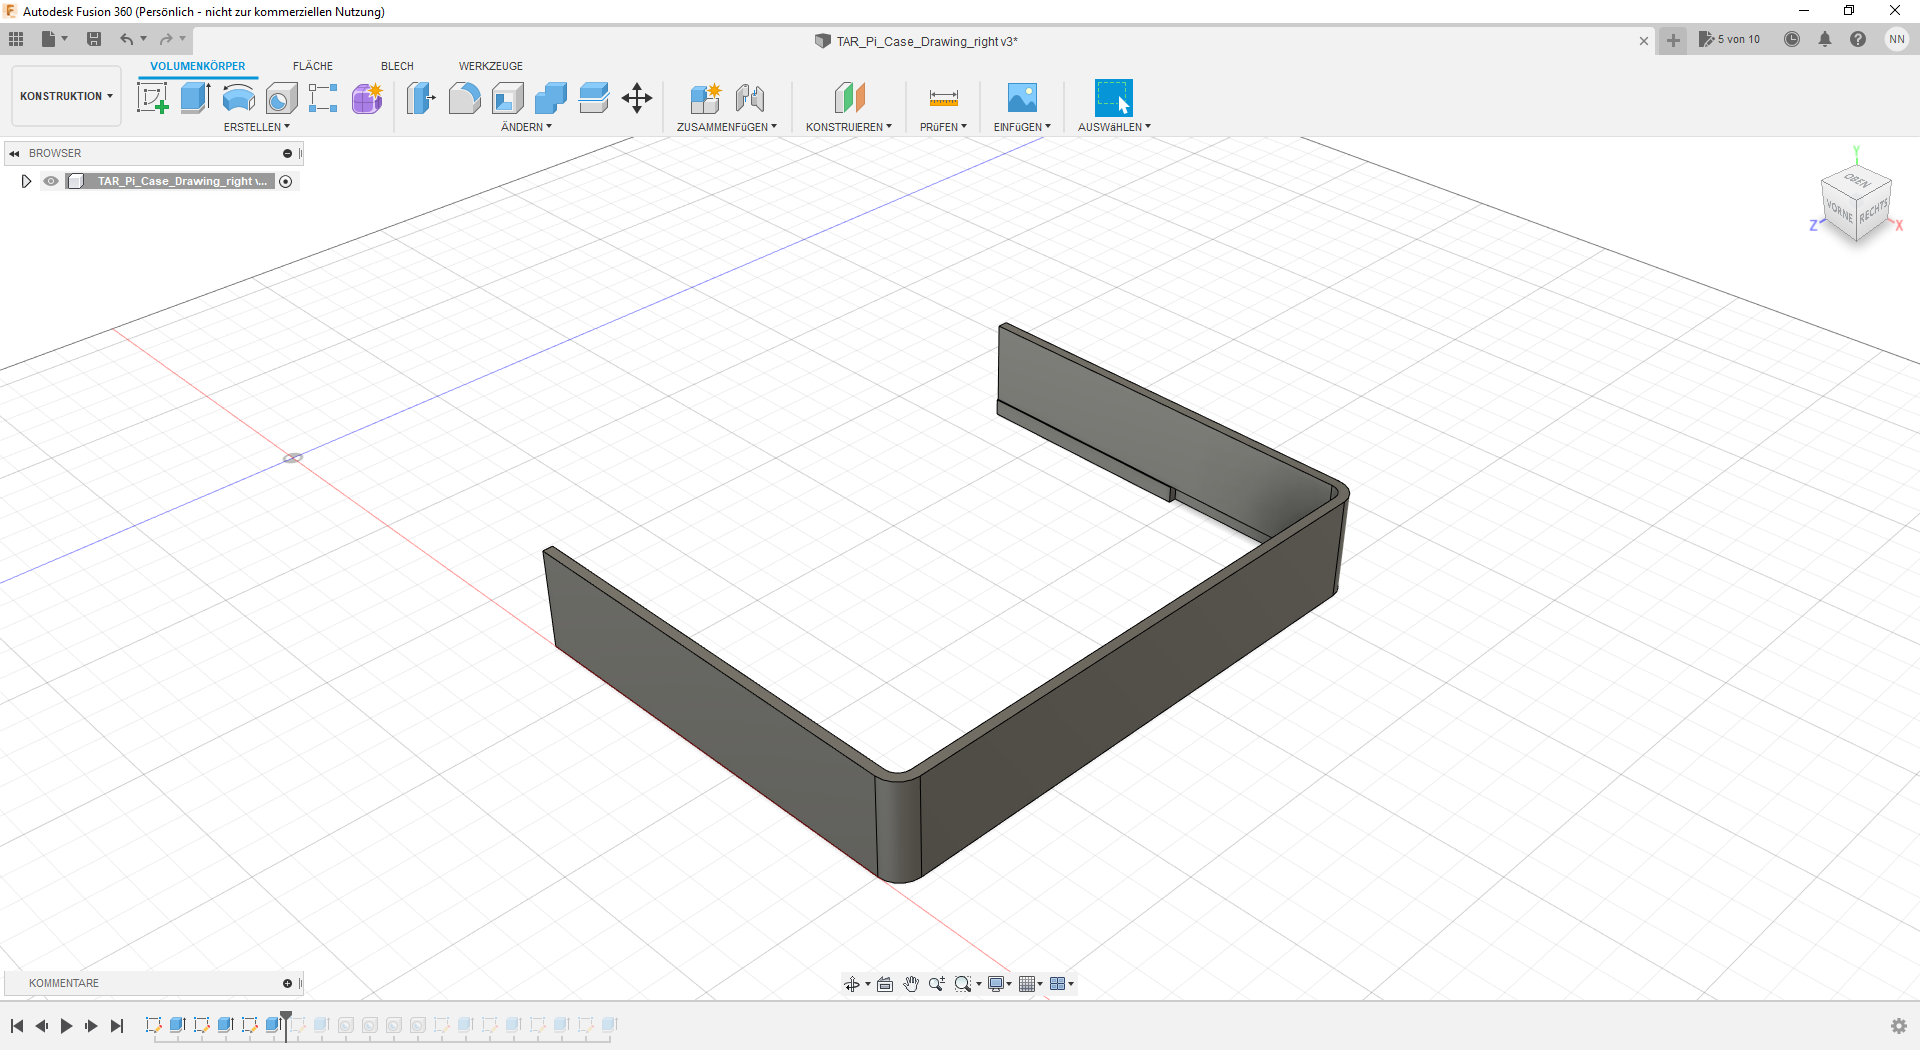
\includegraphics[width=\linewidth]{img/konstruktion_gehaeuse_rechts_005.png}
		\caption[]{}
		\label{fig:design-right-05}
	\end{subfigure}
	\begin{subfigure}[t]{.3\linewidth}
		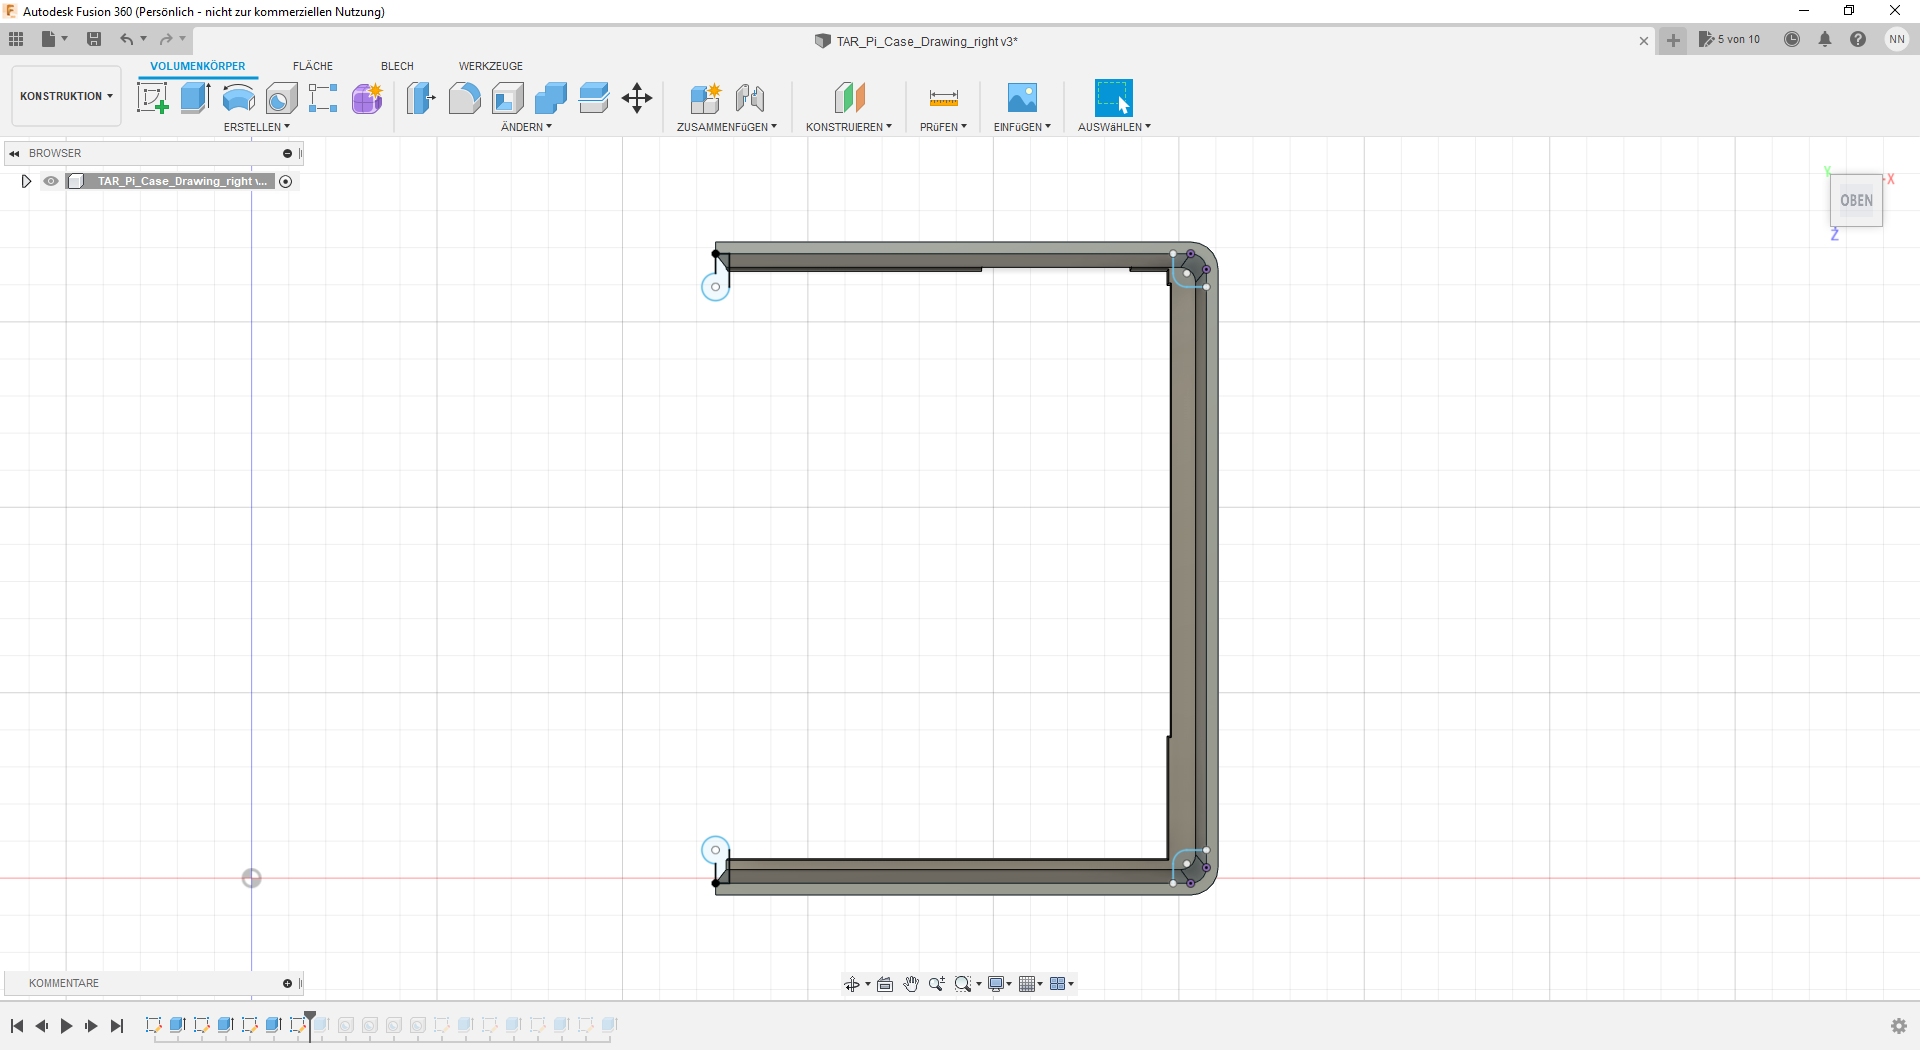
\includegraphics[width=\linewidth]{img/konstruktion_gehaeuse_rechts_006.png}
		\caption[]{}
		\label{fig:design-right-06}
	\end{subfigure}
	\begin{subfigure}[t]{.3\linewidth}
		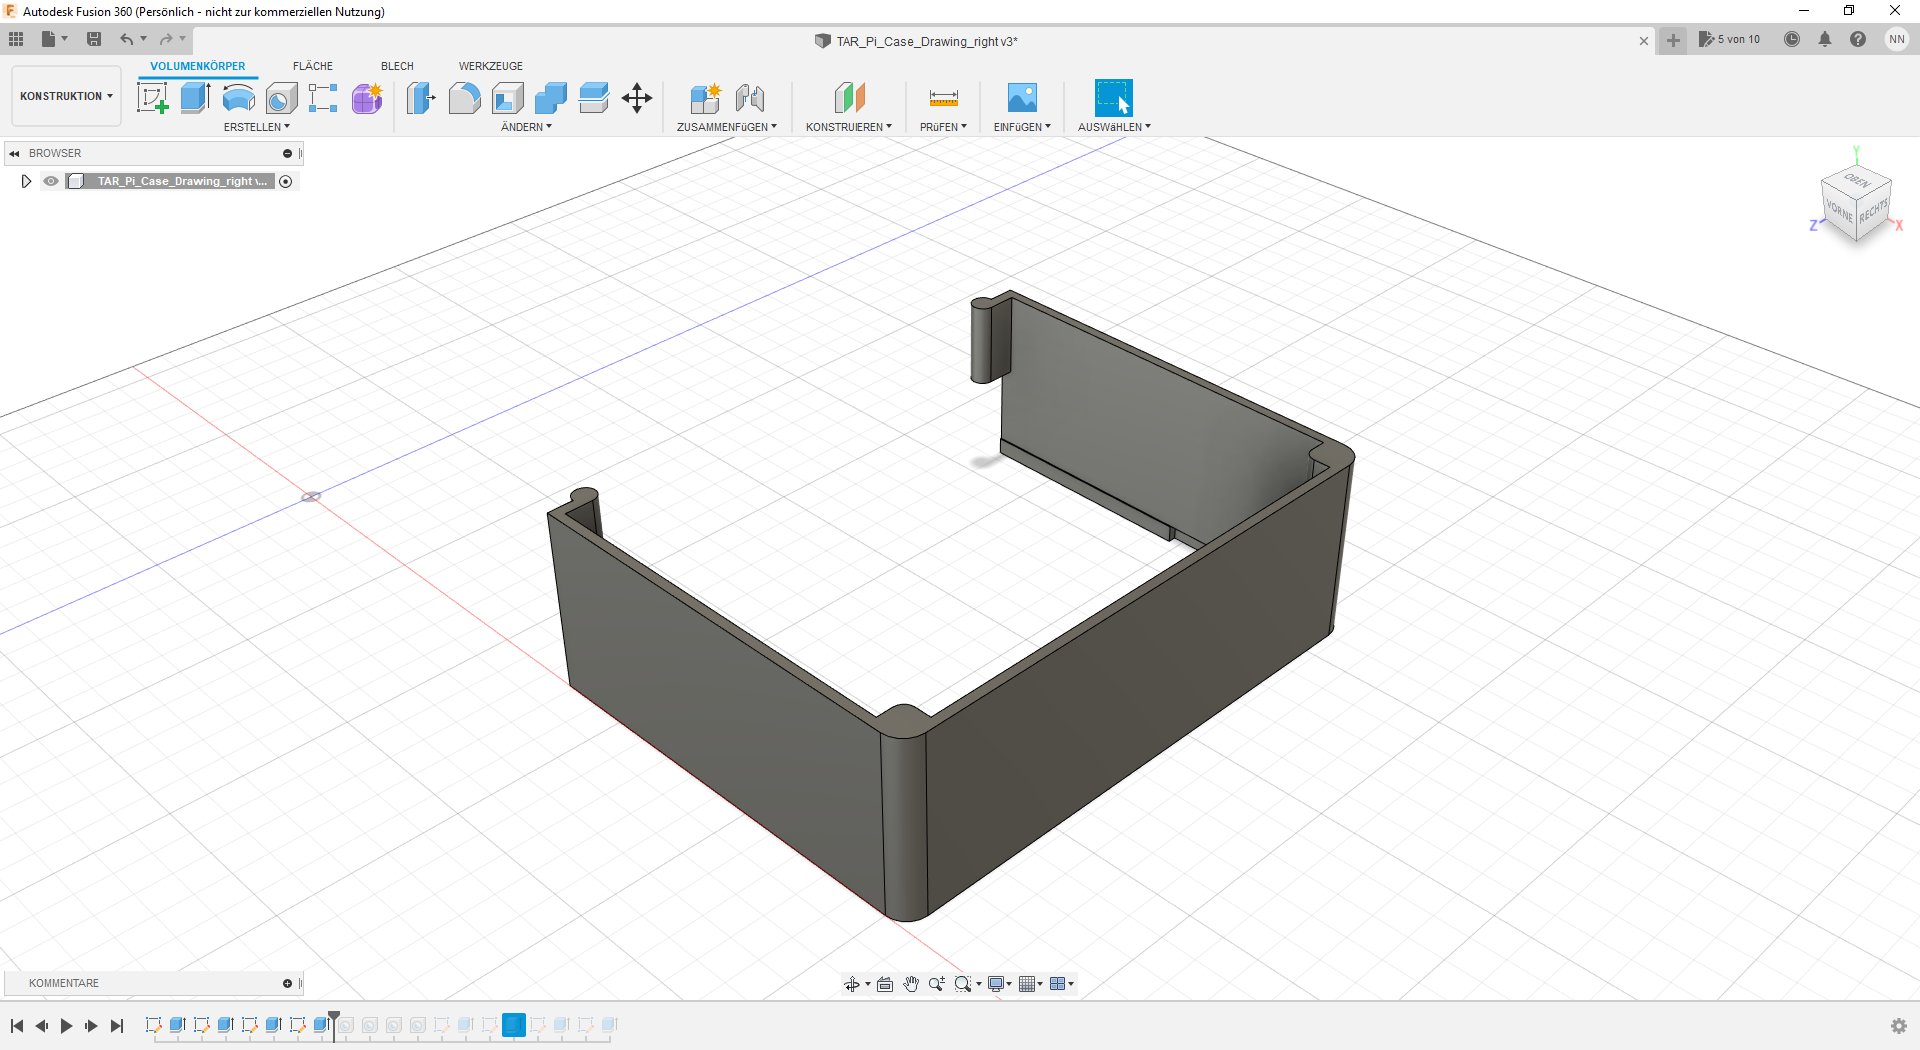
\includegraphics[width=\linewidth]{img/konstruktion_gehaeuse_rechts_007.png}
		\caption[]{}
		\label{fig:design-right-07}
	\end{subfigure}
	\begin{subfigure}[t]{.3\linewidth}
		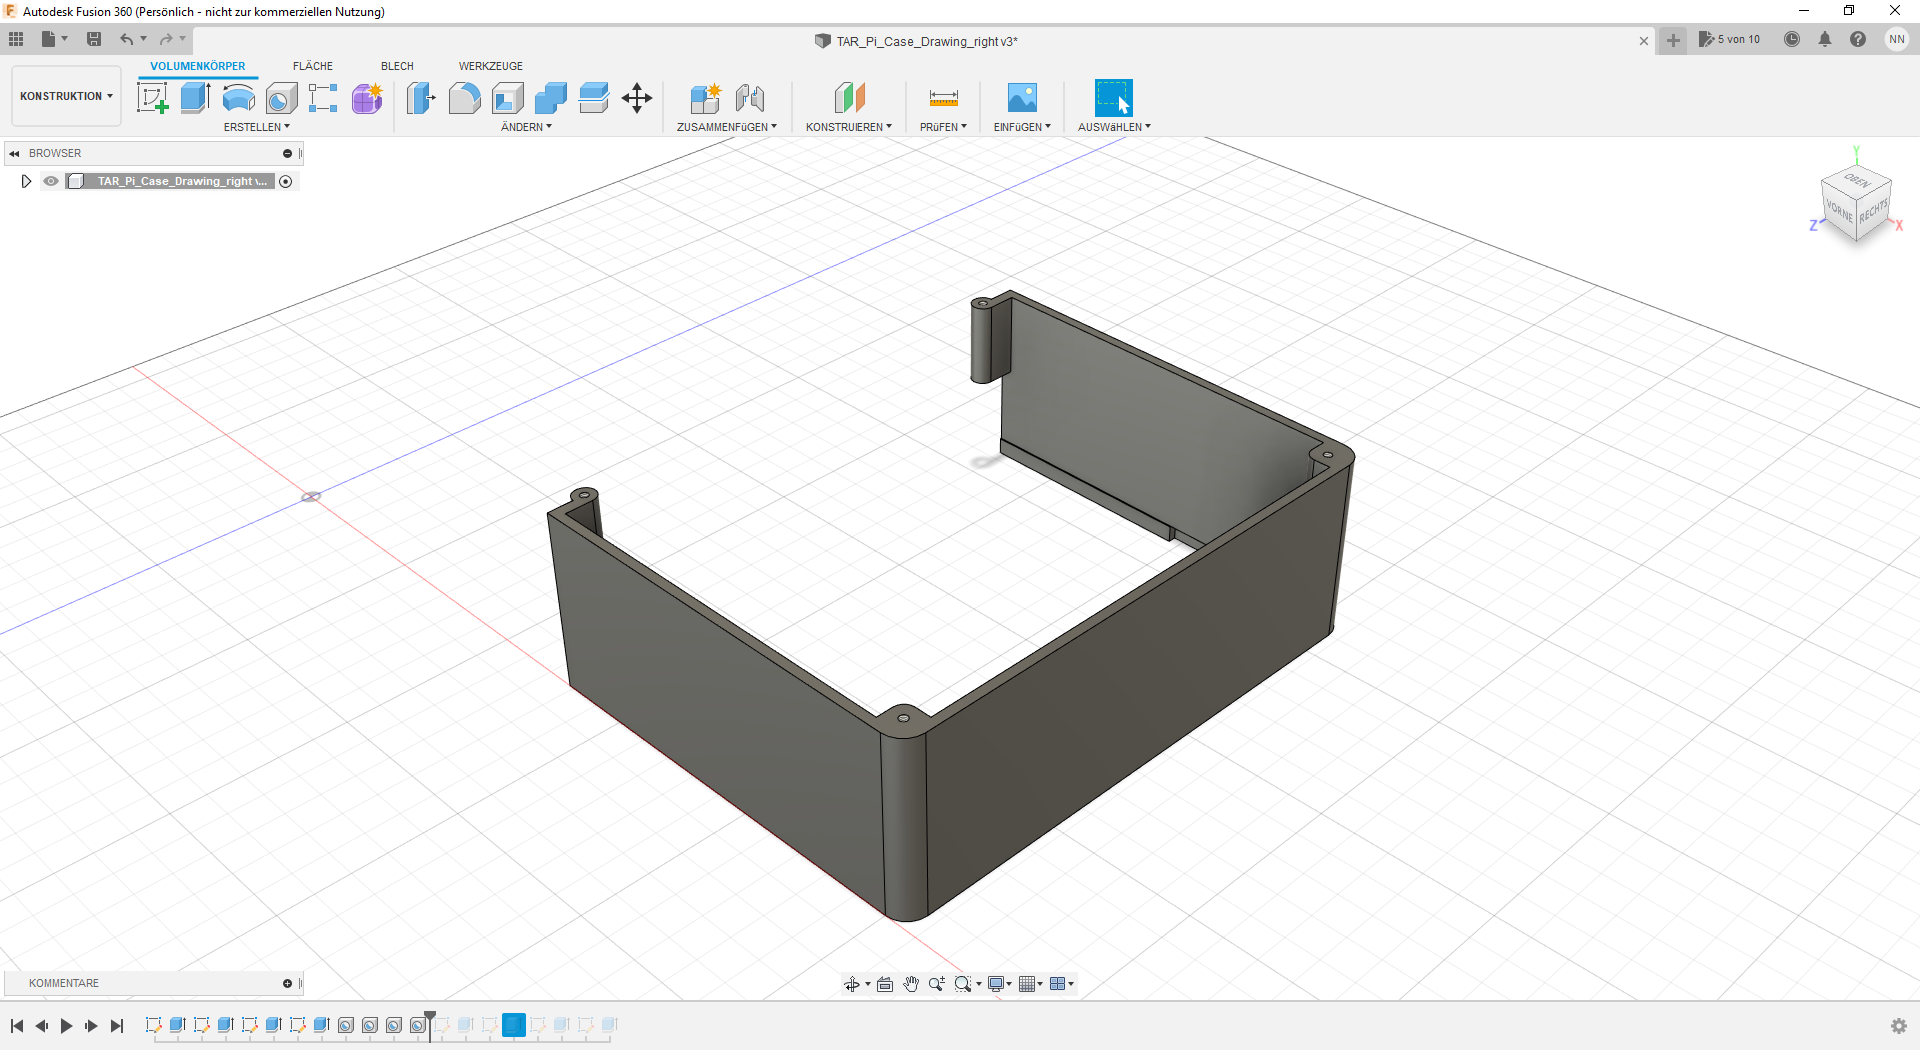
\includegraphics[width=\linewidth]{img/konstruktion_gehaeuse_rechts_008.png}
		\caption[]{}
		\label{fig:design-right-08}
	\end{subfigure}
	\begin{subfigure}[t]{.3\linewidth}
		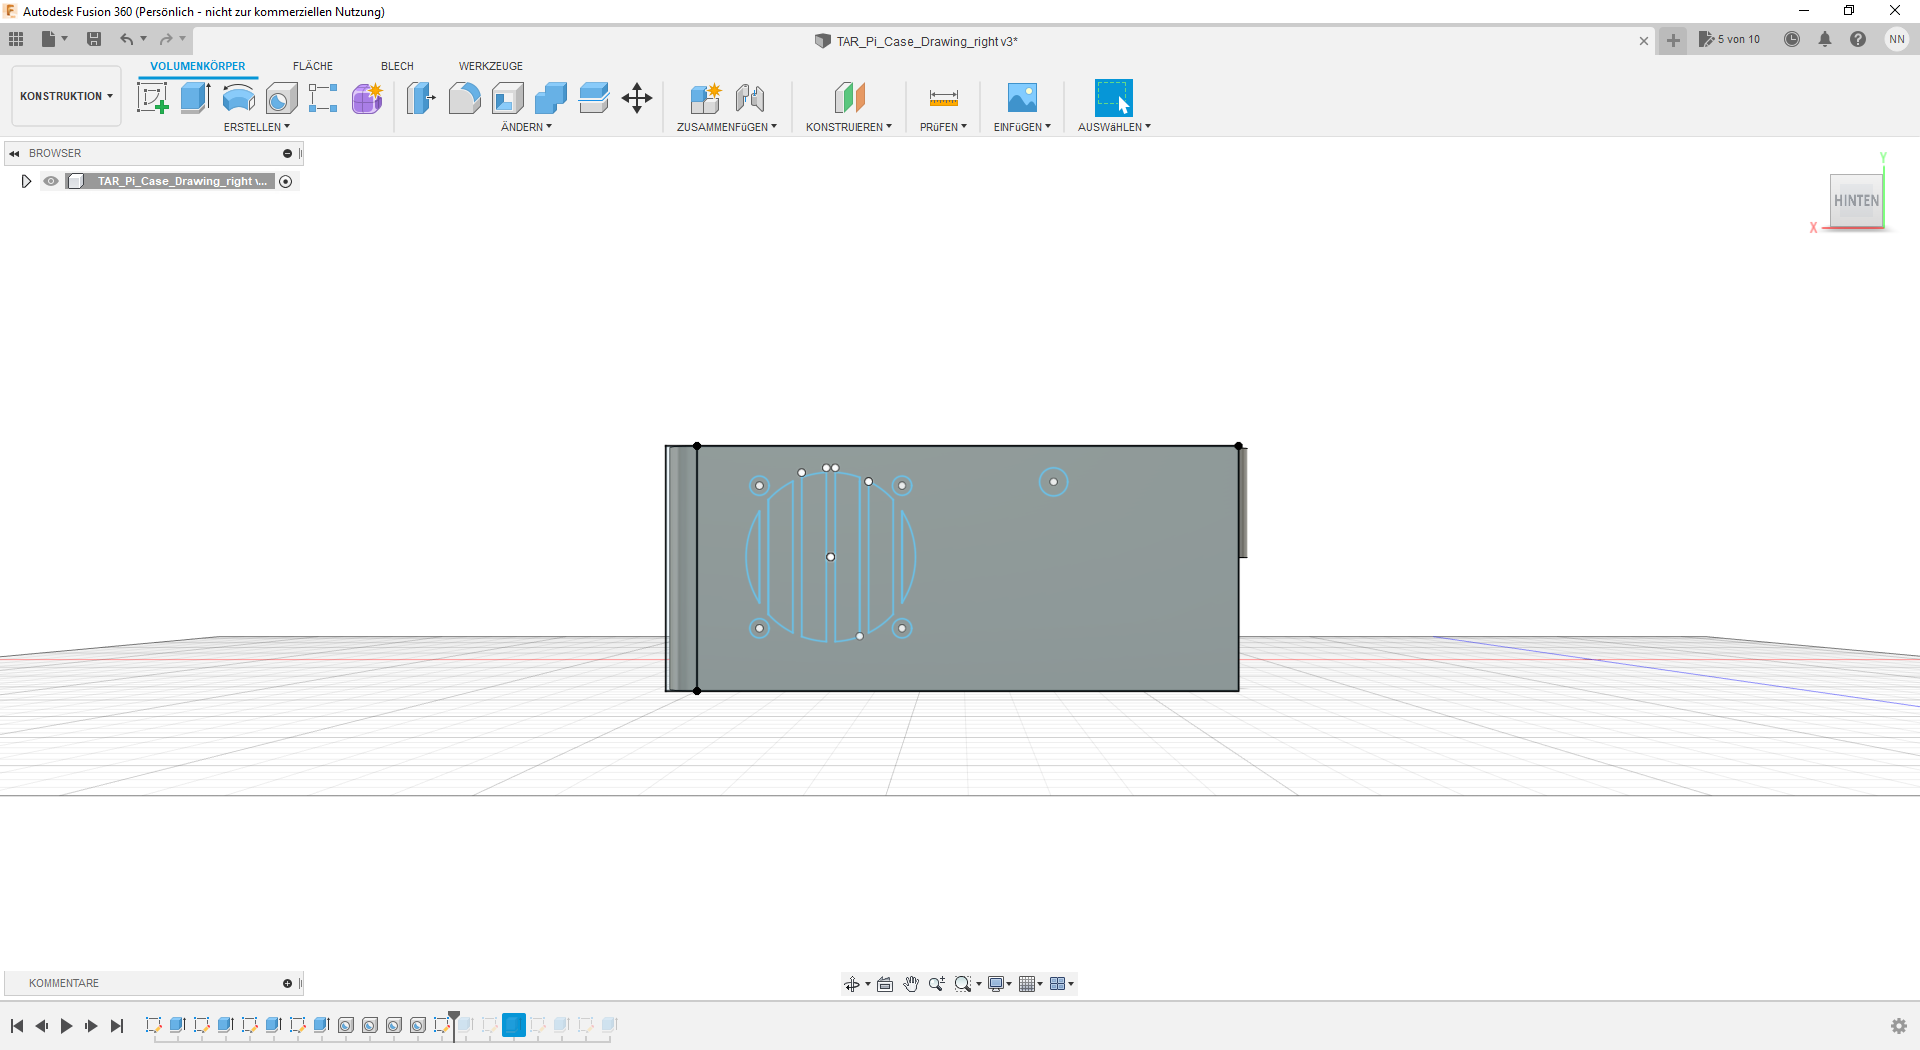
\includegraphics[width=\linewidth]{img/konstruktion_gehaeuse_rechts_009.png}
		\caption[]{}
		\label{fig:design-right-09}
	\end{subfigure}
	\begin{subfigure}[t]{.3\linewidth}
		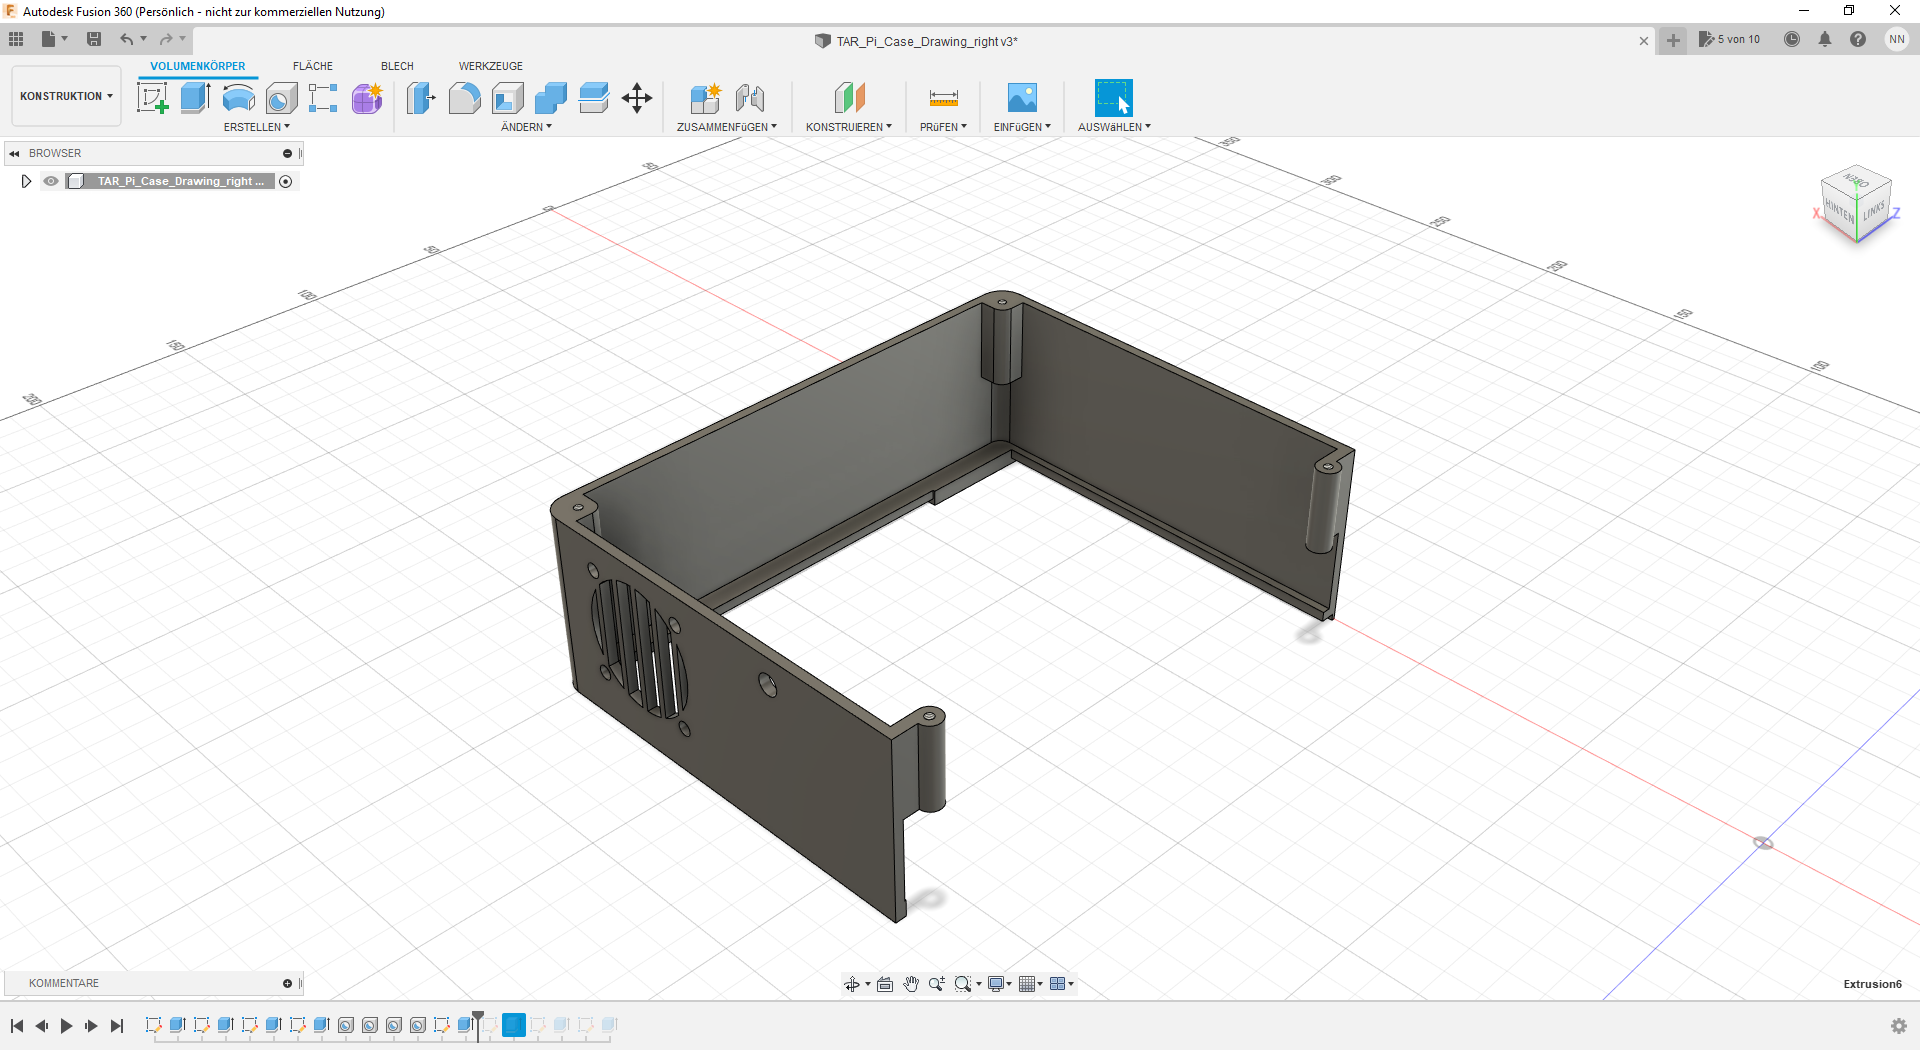
\includegraphics[width=\linewidth]{img/konstruktion_gehaeuse_rechts_010.png}
		\caption[]{}
		\label{fig:design-right-10}
	\end{subfigure}
	\begin{subfigure}[t]{.3\linewidth}
		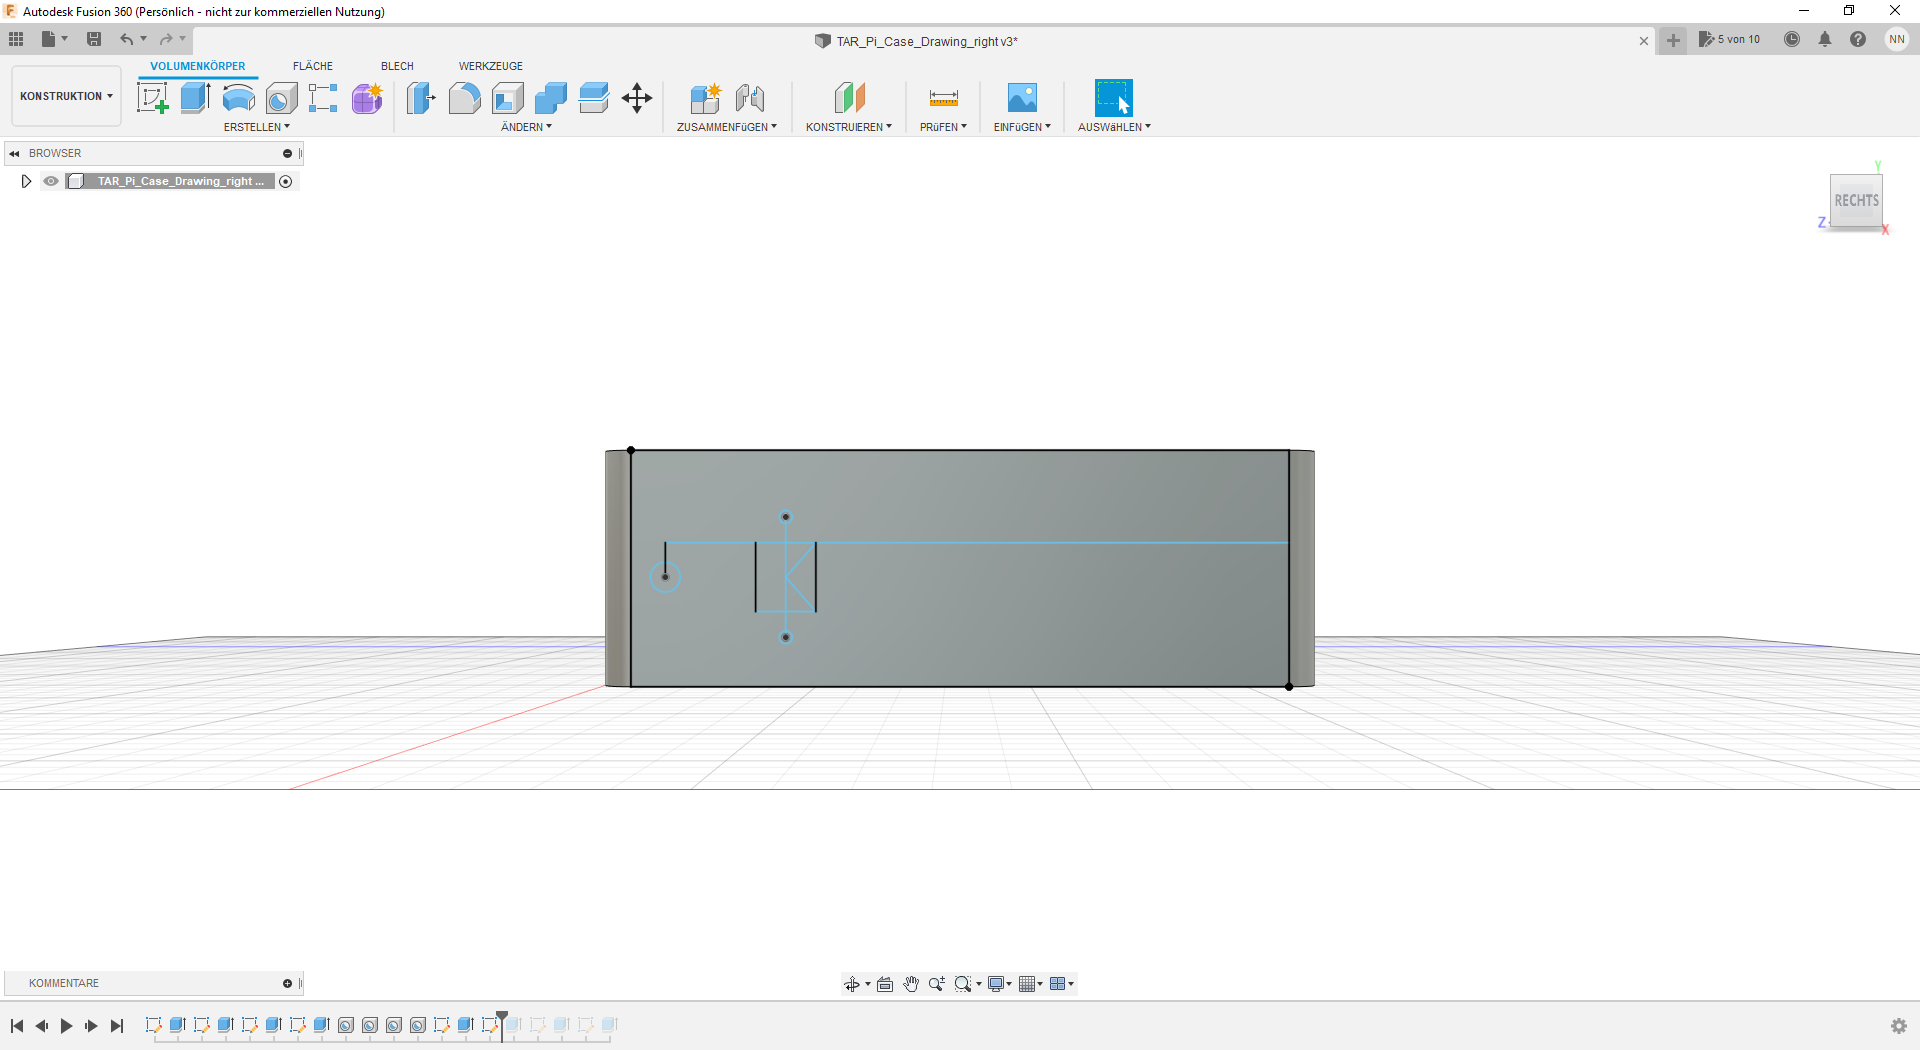
\includegraphics[width=\linewidth]{img/konstruktion_gehaeuse_rechts_011.png}
		\caption[]{}
		\label{fig:design-right-11}
	\end{subfigure}
	\begin{subfigure}[t]{.3\linewidth}
		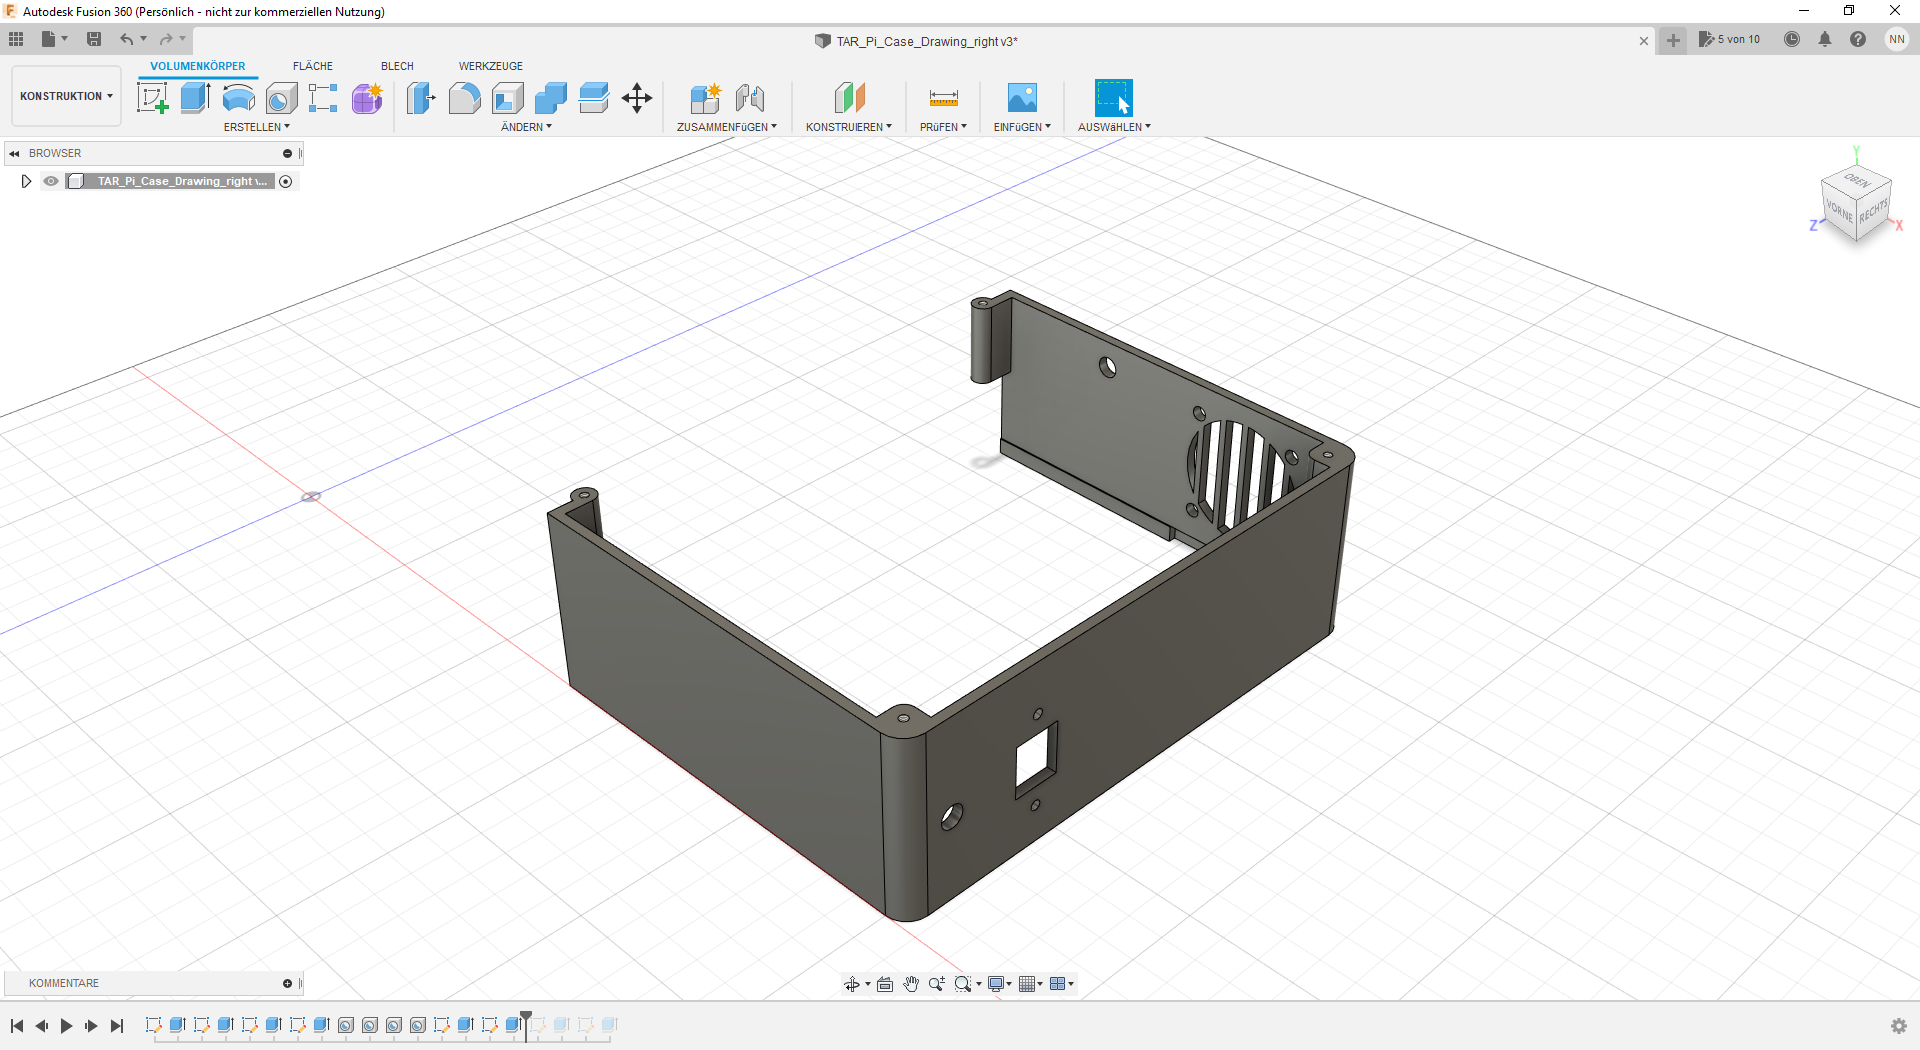
\includegraphics[width=\linewidth]{img/konstruktion_gehaeuse_rechts_012.png}
		\caption[]{}
		\label{fig:design-right-12}
	\end{subfigure}
	\begin{subfigure}[t]{.3\linewidth}
		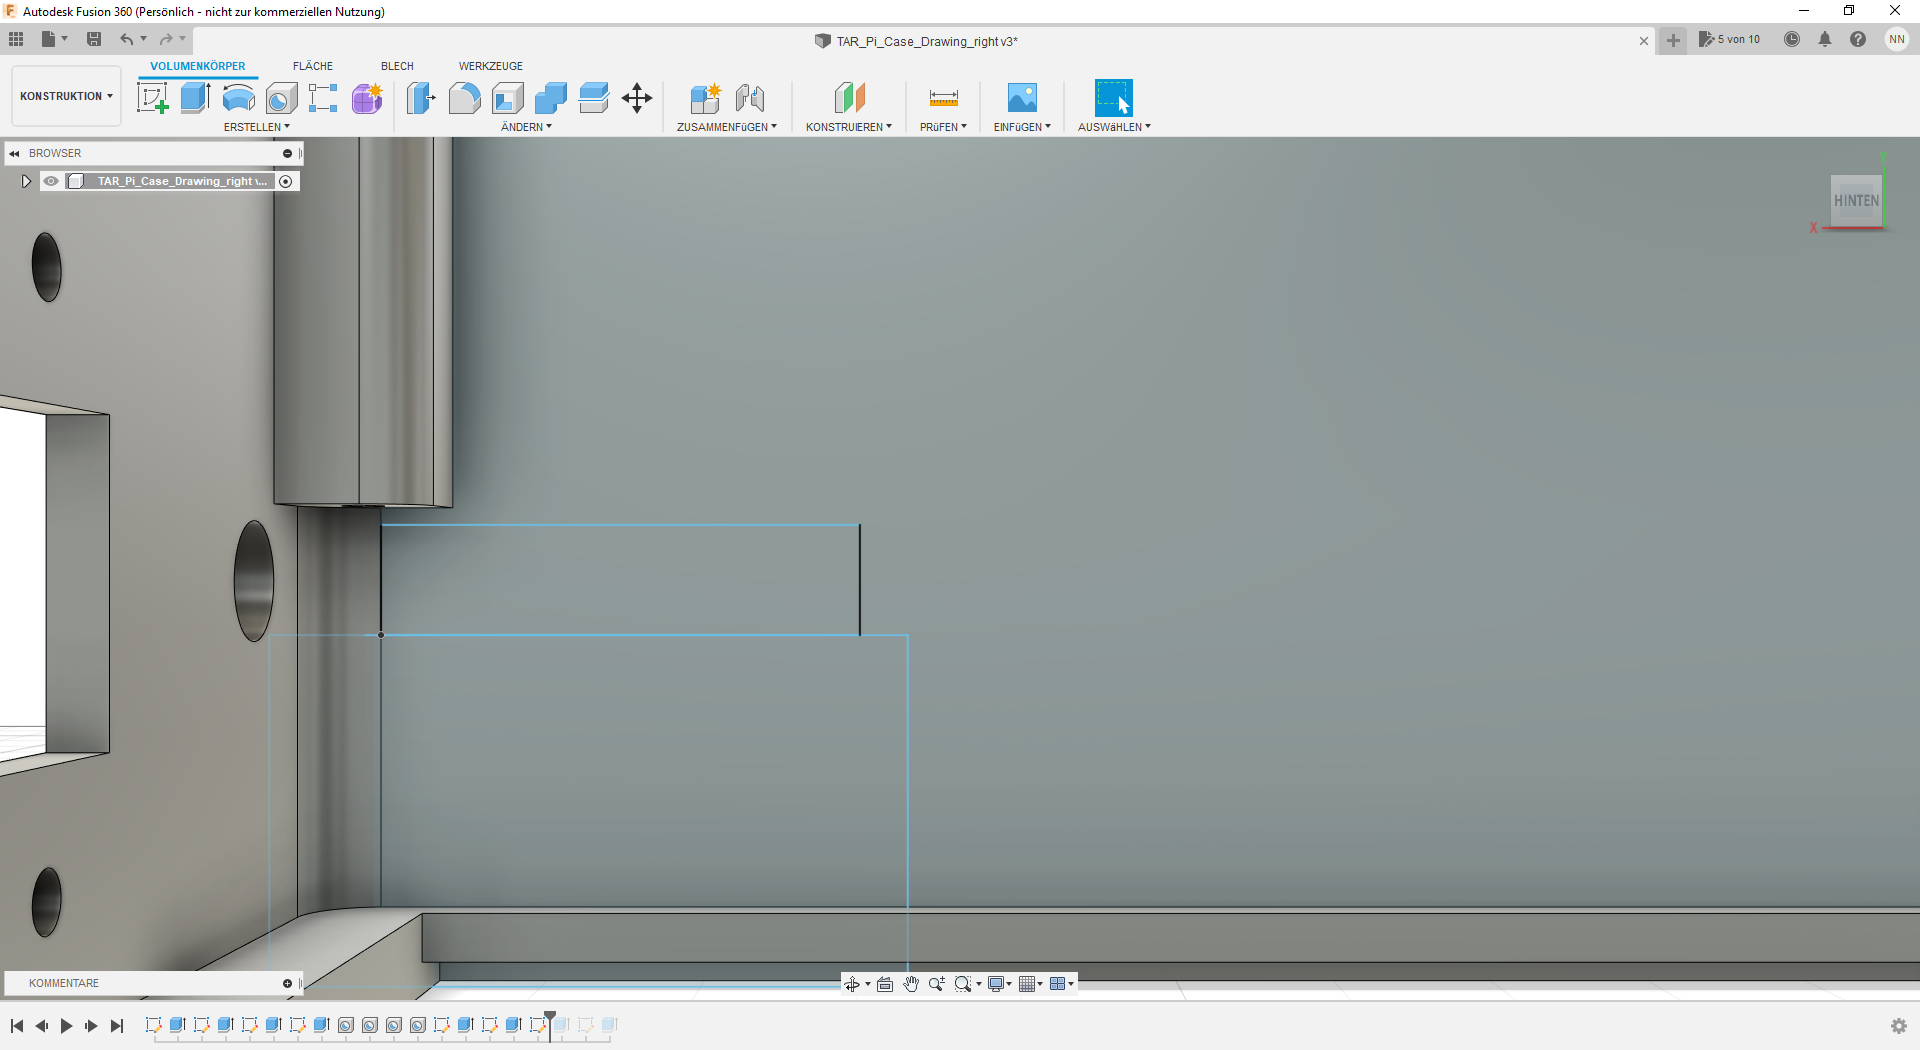
\includegraphics[width=\linewidth]{img/konstruktion_gehaeuse_rechts_013.png}
		\caption[]{}
		\label{fig:design-right-13}
	\end{subfigure}
	\begin{subfigure}[t]{.3\linewidth}
		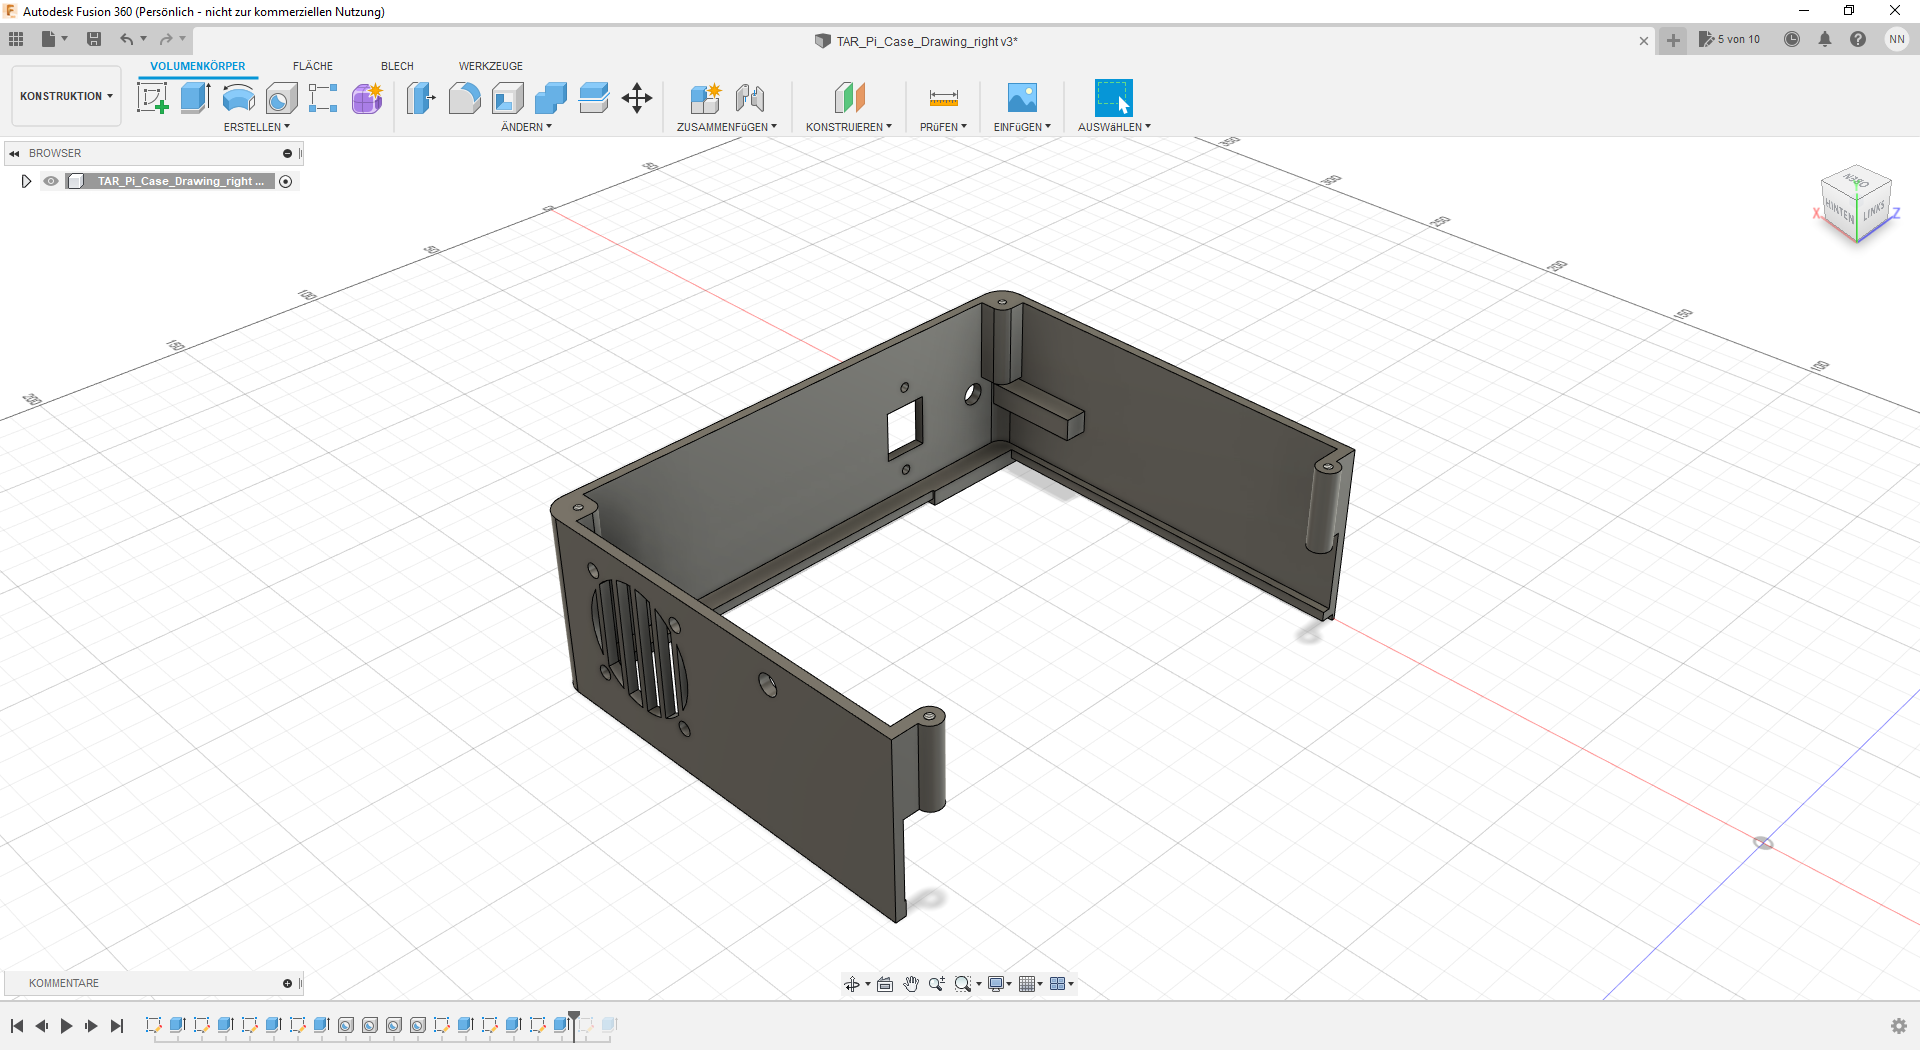
\includegraphics[width=\linewidth]{img/konstruktion_gehaeuse_rechts_014.png}
		\caption[]{}
		\label{fig:design-right-14}
	\end{subfigure}
	\begin{subfigure}[t]{.3\linewidth}
		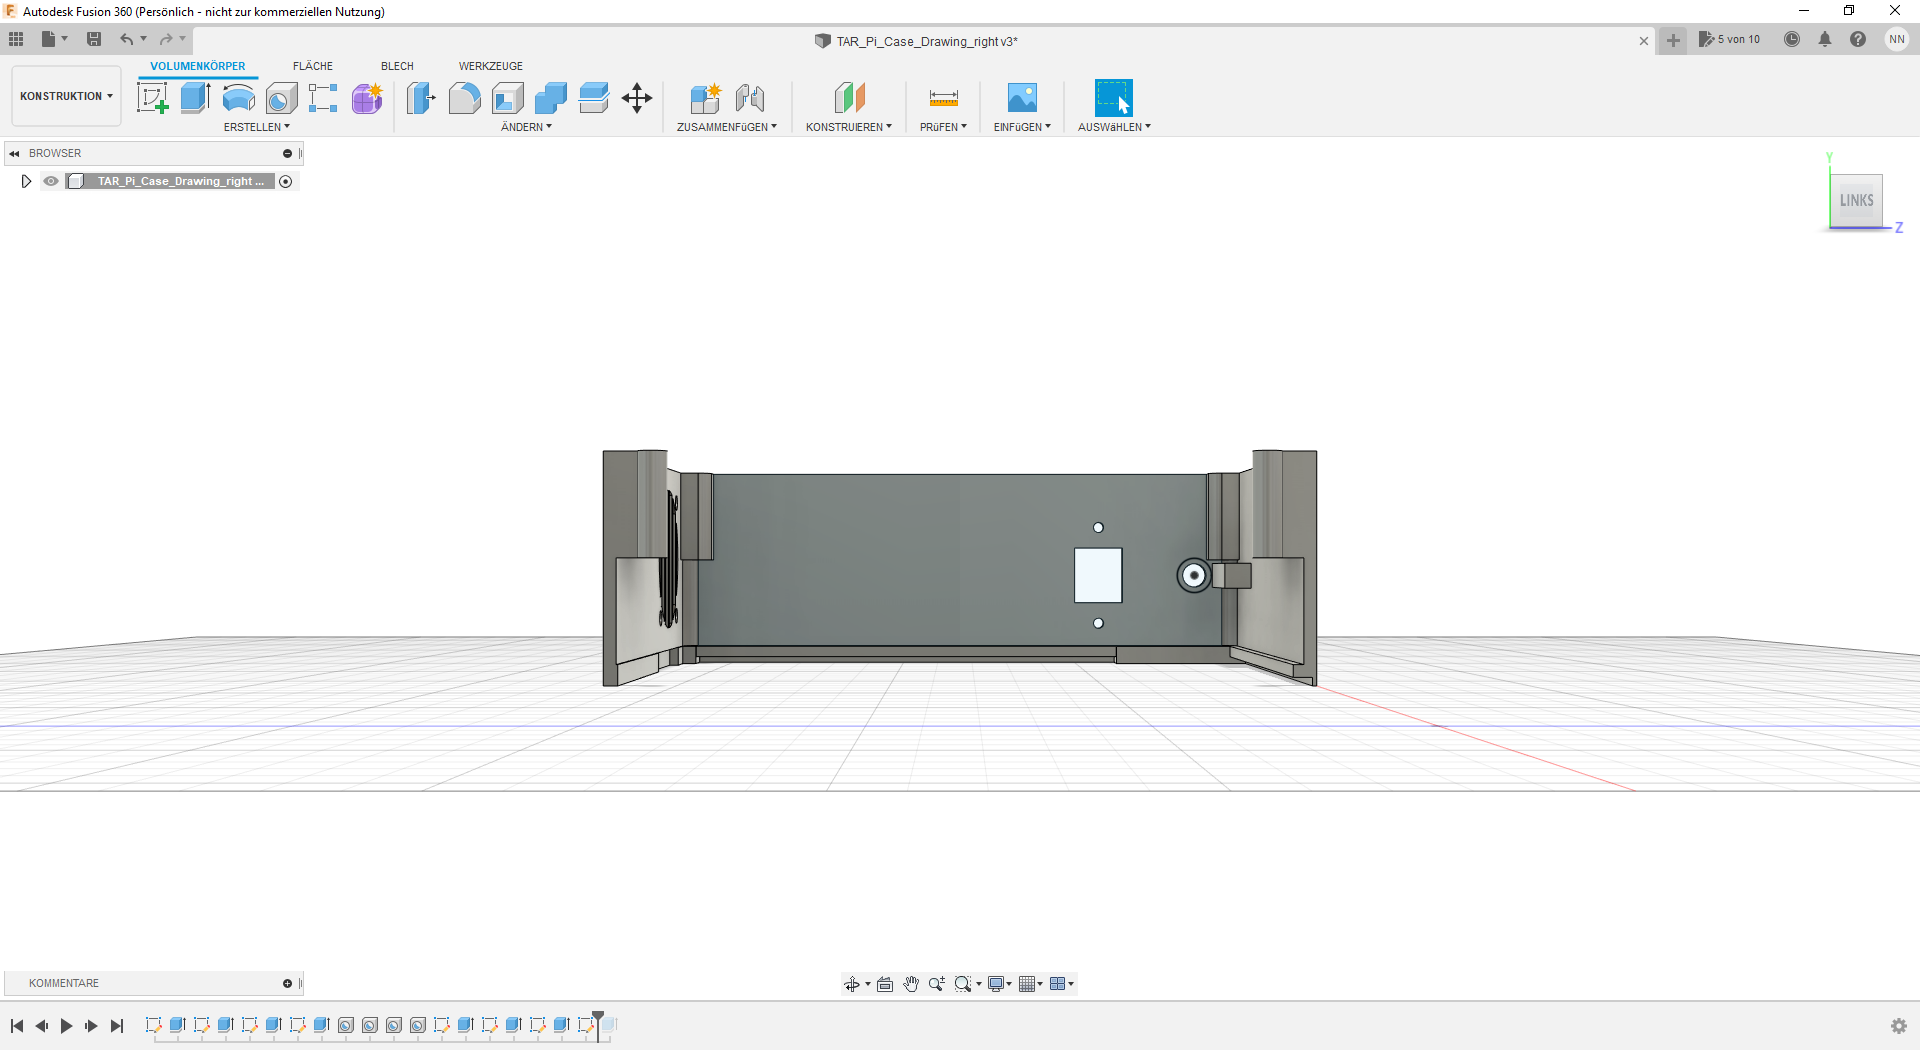
\includegraphics[width=\linewidth]{img/konstruktion_gehaeuse_rechts_015.png}
		\caption[]{}
		\label{fig:design-right-15}
	\end{subfigure}
	\begin{subfigure}[t]{.3\linewidth}
		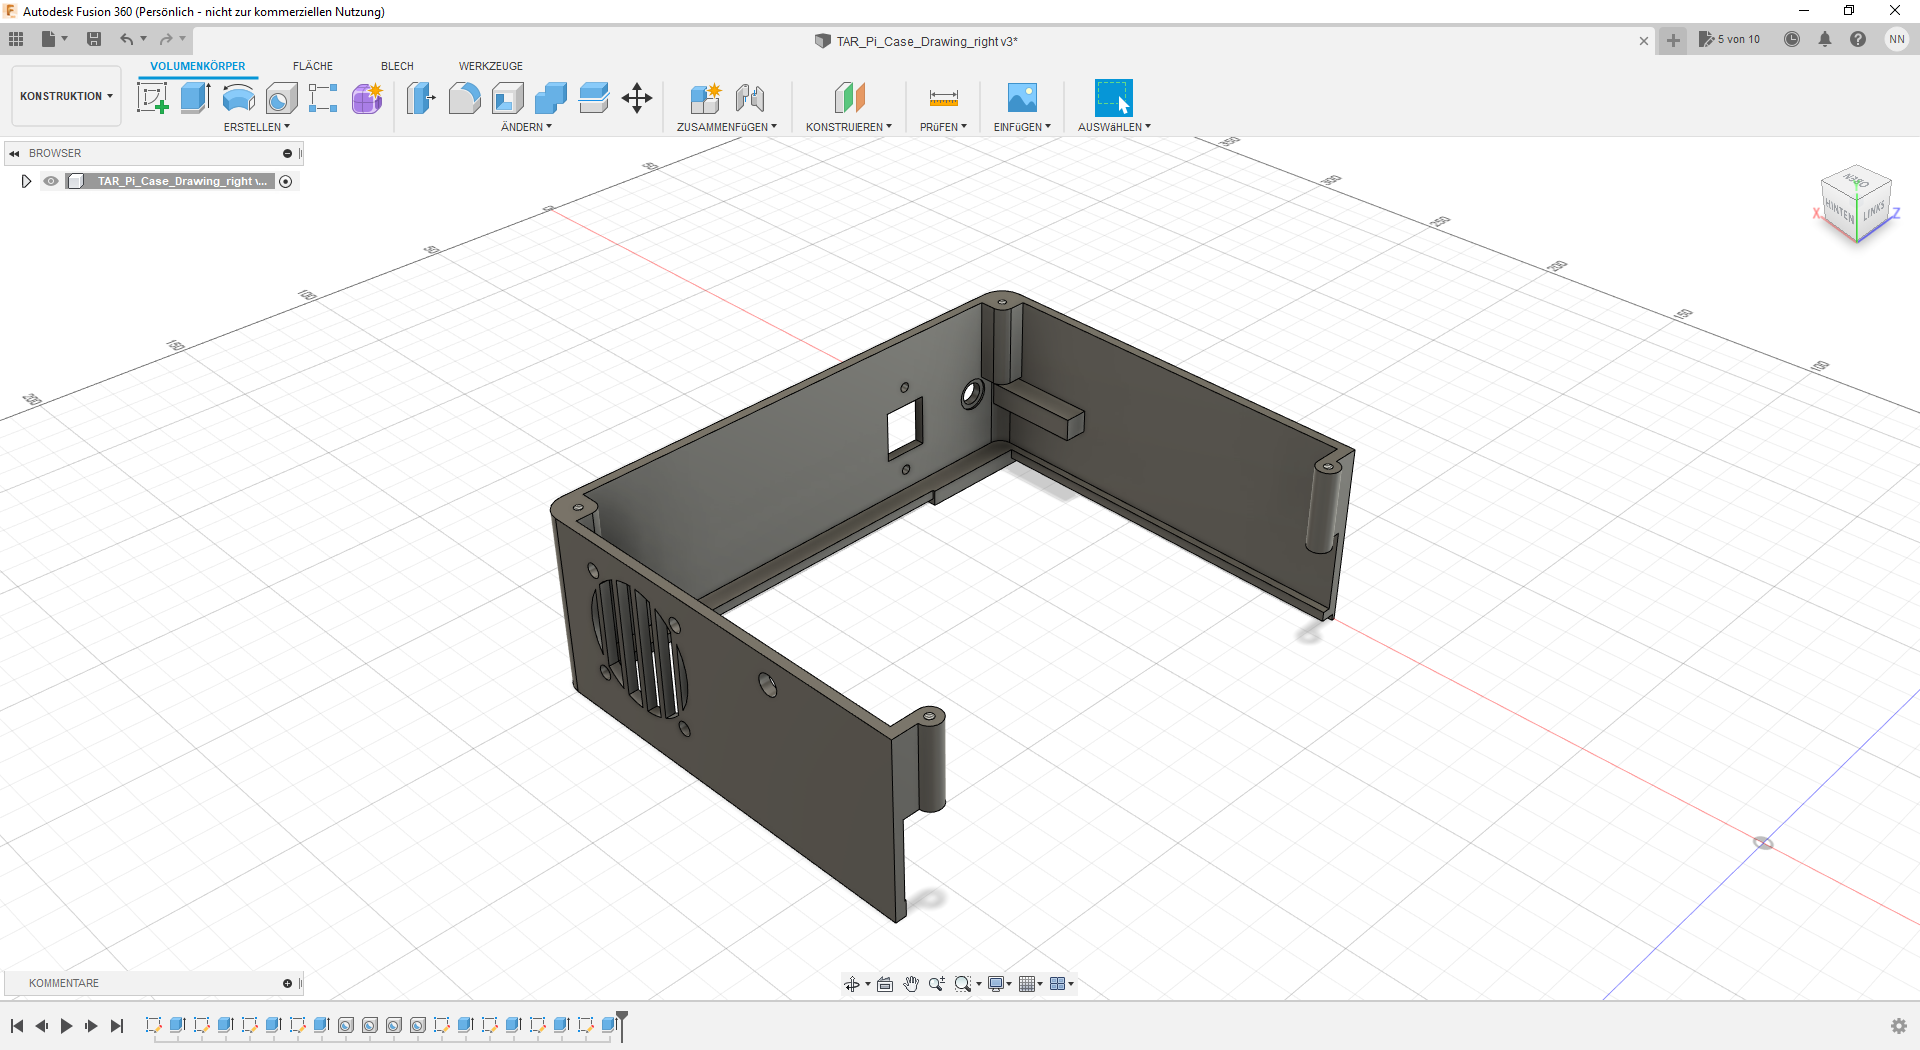
\includegraphics[width=\linewidth]{img/konstruktion_gehaeuse_rechts_016.png}
		\caption[]{}
		\label{fig:design-right-16}
	\end{subfigure}
	\caption[Entwurf des rechten Wandteils]{Entwurf des rechten Wandteils}
	\label{fig:design-right}
\end{figure}\par
\paragraph{Gehäuserückwand}
Das Design der Gehäuserückwand basiert nur rudimentär auf der in \ref{fig:design-case-base} erstellten Zeichnung. Die Außenmaße Stimmen zwar überein, die Zeichnung für die Auflage auf den Seitenwänden musste aber neu erstellt werden. Zusätzlich wurde eine Diagonale zur punktsymmetrischen Trennung der Teile eingefügt (vgl. \ref{fig:design-back-01}), welche die Zeit für die Konstruktion von zwei unterschiedlichen Teilen für die Rückseite reduzieren soll. Die Zeichnung wurde dann entsprechend extrudiert (vgl. \ref{fig:design-back-02}). Um die Teile nach dem Druck besser verbinden zu können, wurde ein Vorsprung auf der kurzen Seite des Bauteils extruiert (vgl. \ref{fig:design-back-03}). Um beim Druck Material zu sparen, wurde ein weiter Teil der Innenzeichnung ins Negative extruiert, um den Bereich freizustellen (vgl. \ref{fig:design-back-04}). Für evetuelle Toleranzen zwischen den beiden Teilen wurde auf dem Vorsprung die Aussparung für die unterliegende Schraubendurchführung erhöht (vgl. \ref{fig:design-back-05}). Zusätzlich wurde der Vorsprung von unten mit einer Phase versehen, um die Materialnutzung für das Teil weiter zu reduzieren (vgl. \ref{fig:design-back-06}). Des weiteren wurde an die obere Kante (vgl. \ref{fig:design-back-07}) und an die Innenkante (vgl. \ref{fig:design-back-08}) mit einer Phase versehen. Eine ähnliche Phase wurde auch an dem Vorsprung angebracht (vgl. \ref{fig:design-back-09}). Um die Bohrung am die richtige Stelle zu setzen, wurde eine Hilfzeichnung auf die Außenfläche gesetzt (vgl. \ref{fig:design-back-10}). Anschließend wurden drei M3-Bohrungen für Senkkopfschrauben gesetzt (vgl. \ref{fig:design-back-11}). Um das Gehäuse an der Wand anbringen zu können, wurden eine Zeichnung auf die Oberseite des Gehäuses gelegt (vgl. \ref{fig:design-back-12}) und dann ins Negativ extruiert (vgl. \ref{fig:design-back-13}. Um bei der Anbringung nicht an einen bestimmten Typ Schrauben gebunden zu sein, wurde eine kleine Phase an den engen Teil der Aufhängungslöcher gelegt (vgl. \ref{fig:design-back-14}). Damit bei der Verbindung der beiden Einzelteile die Vorsprünge nicht aneinander stoßen, wurde an den Vorsprung auch eine Phase angelegt (vgl. \ref{fig:design-back-15}).
\begin{figure}[h!tb]
	\begin{subfigure}[t]{.3\linewidth}
		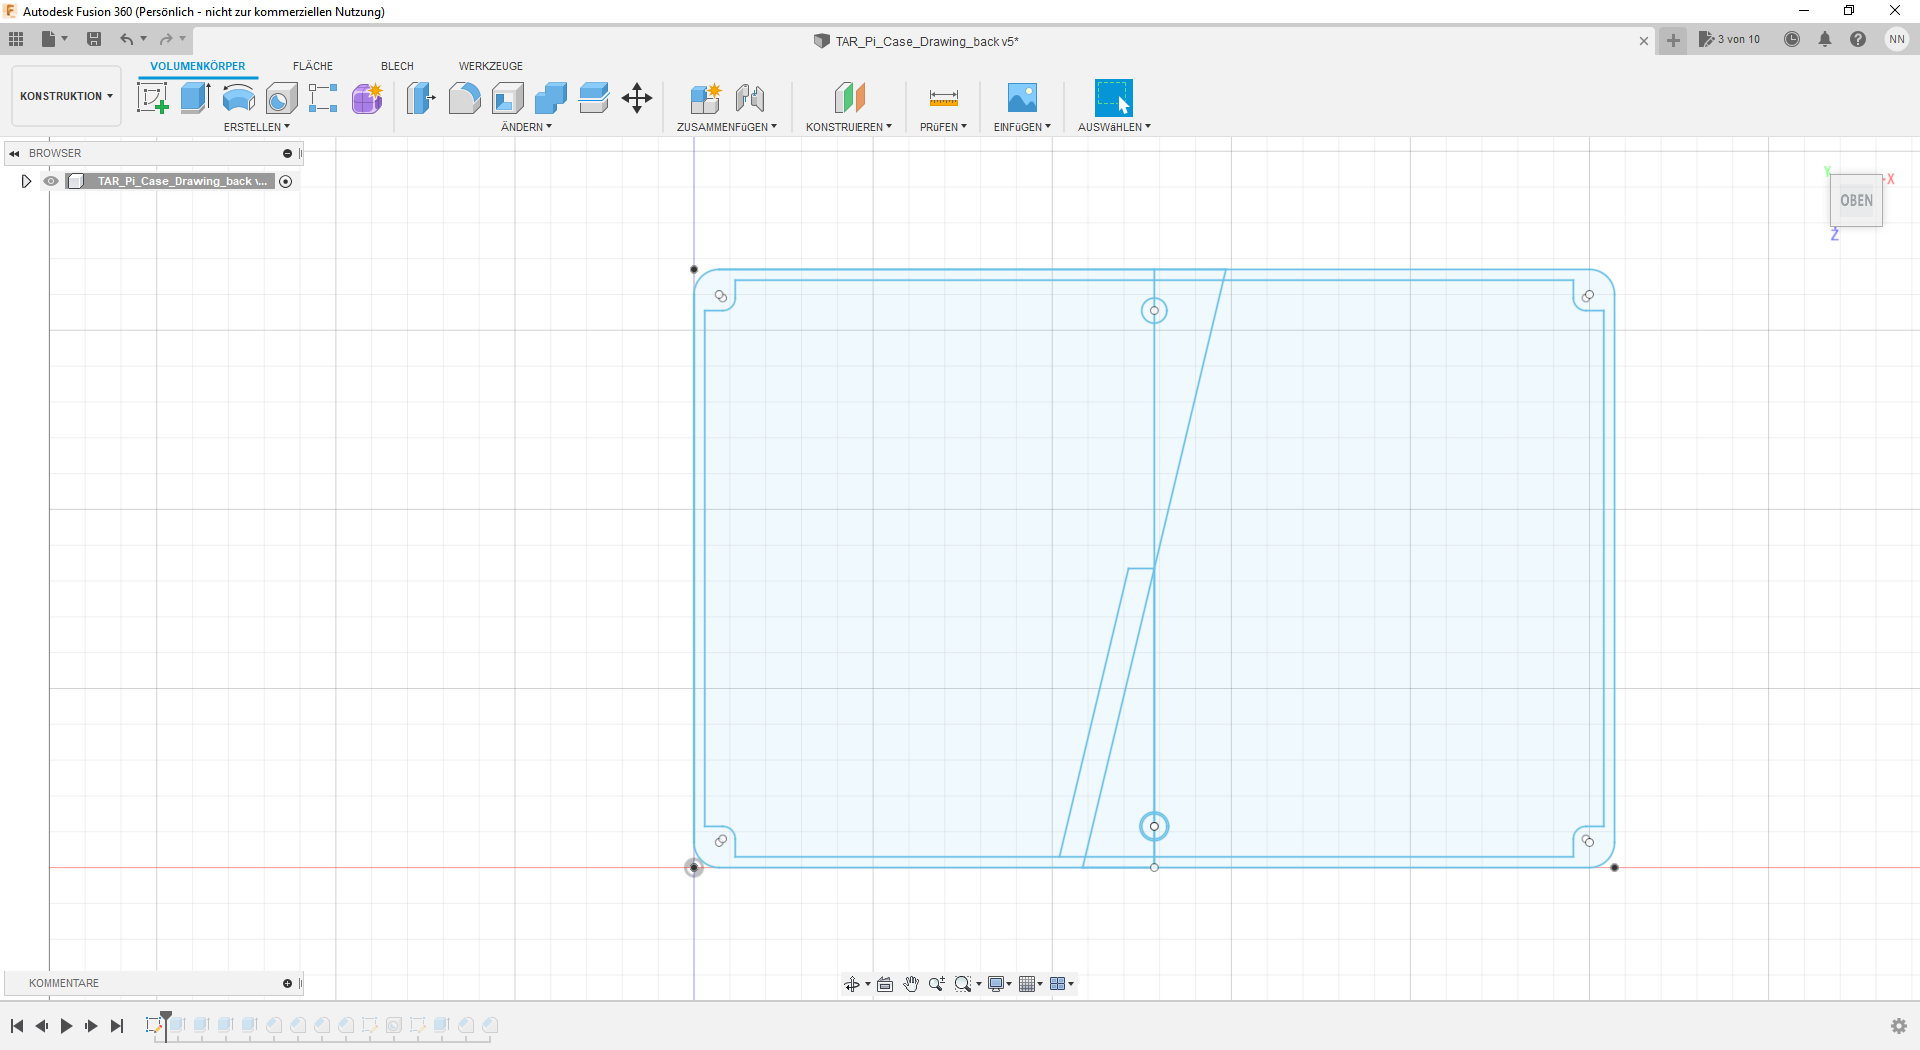
\includegraphics[width=\linewidth]{img/konstruktion_gehaeuse_hinten_001.png}
		\caption[]{}
		\label{fig:design-back-01}
	\end{subfigure}	
	\begin{subfigure}[t]{.3\linewidth}
		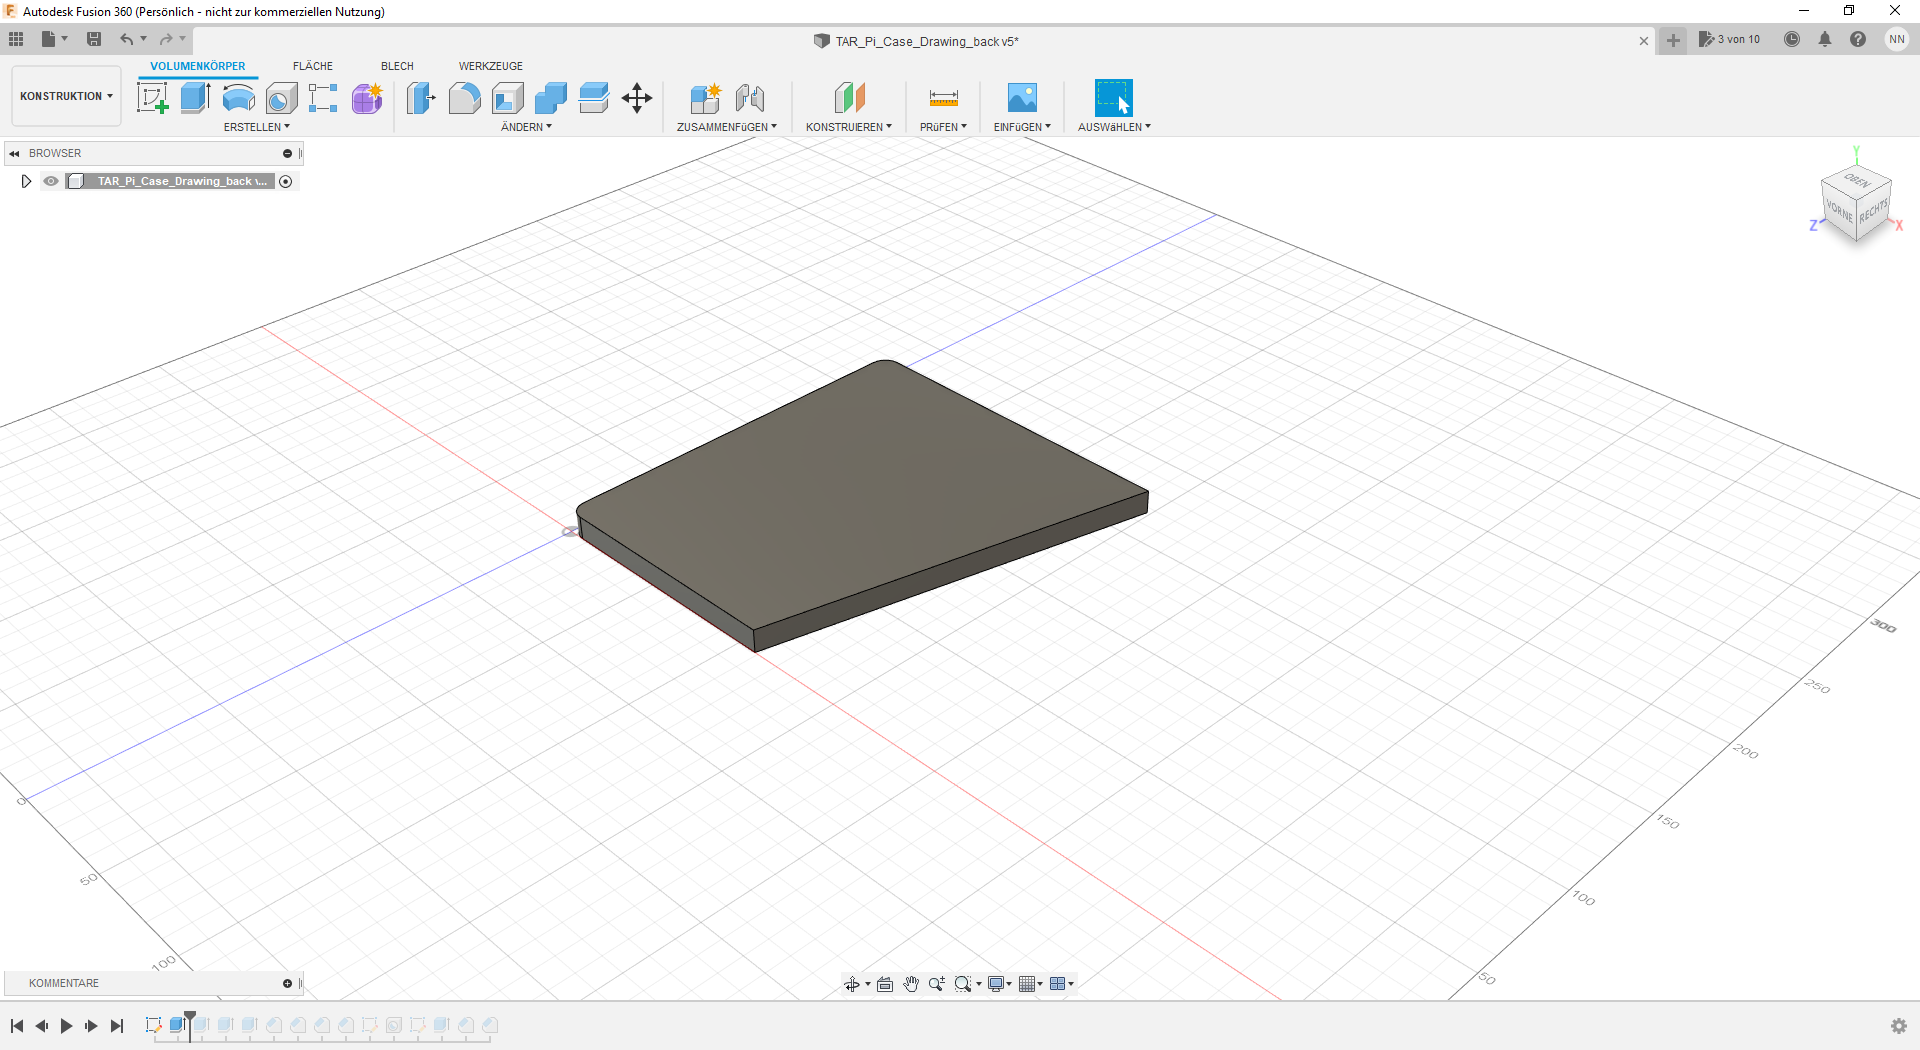
\includegraphics[width=\linewidth]{img/konstruktion_gehaeuse_hinten_002.png}
		\caption[]{}
		\label{fig:design-back-02}
	\end{subfigure}
	\begin{subfigure}[t]{.3\linewidth}
		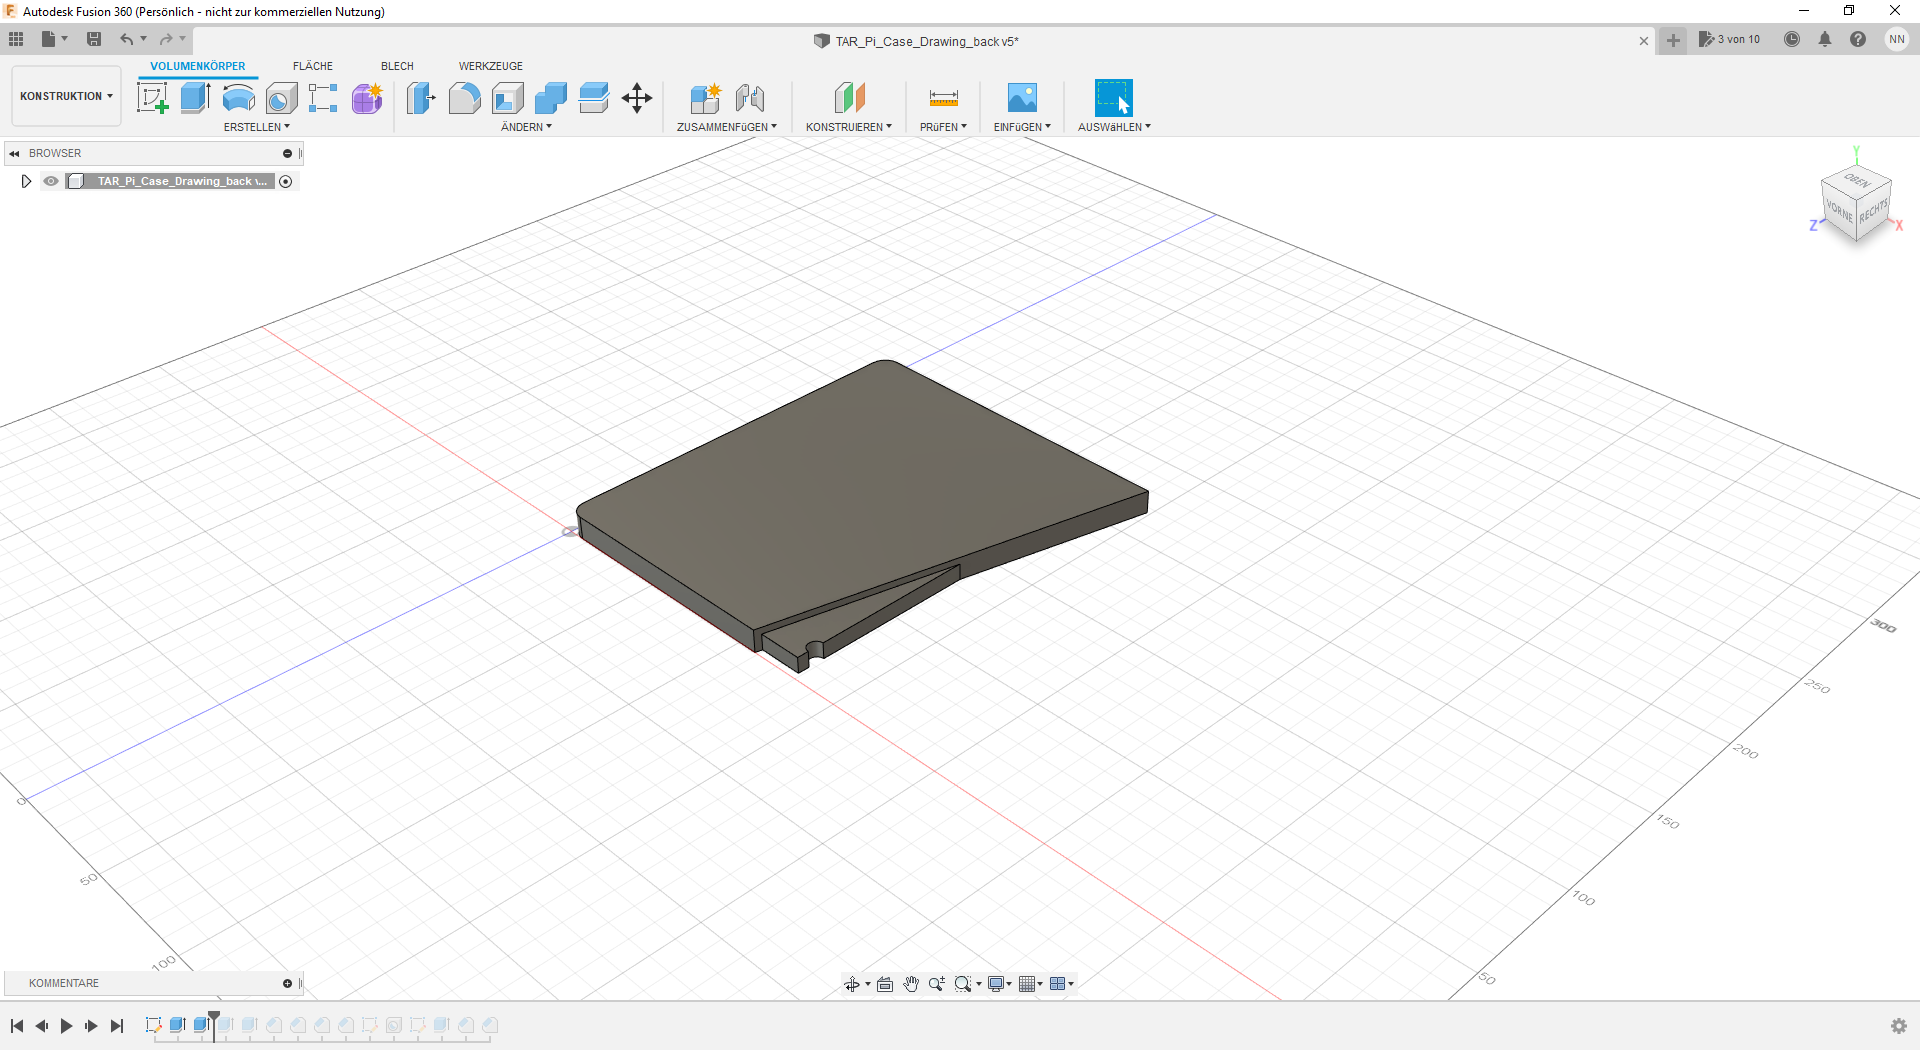
\includegraphics[width=\linewidth]{img/konstruktion_gehaeuse_hinten_003.png}
		\caption[]{}
		\label{fig:design-back-03}
	\end{subfigure}
	\begin{subfigure}[t]{.3\linewidth}
		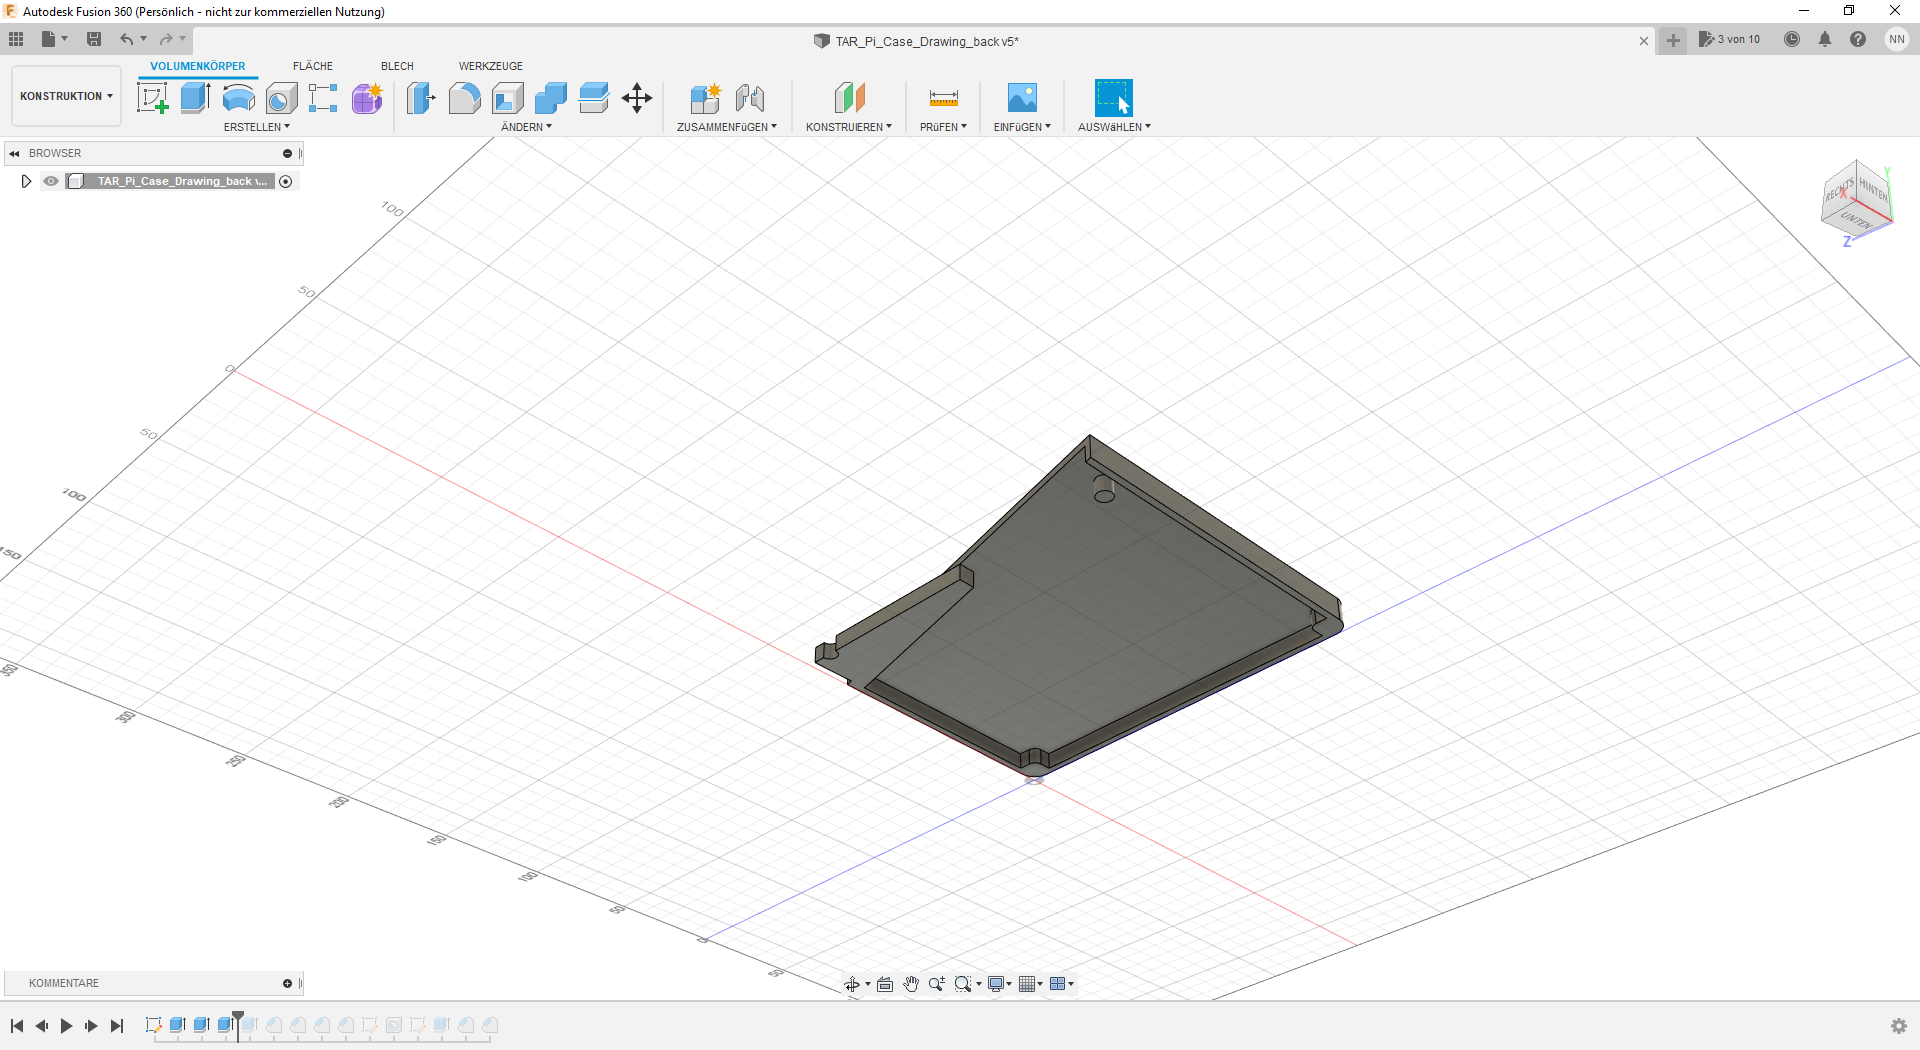
\includegraphics[width=\linewidth]{img/konstruktion_gehaeuse_hinten_004.png}
		\caption[]{}
		\label{fig:design-back-04}
	\end{subfigure}
	\begin{subfigure}[t]{.3\linewidth}
		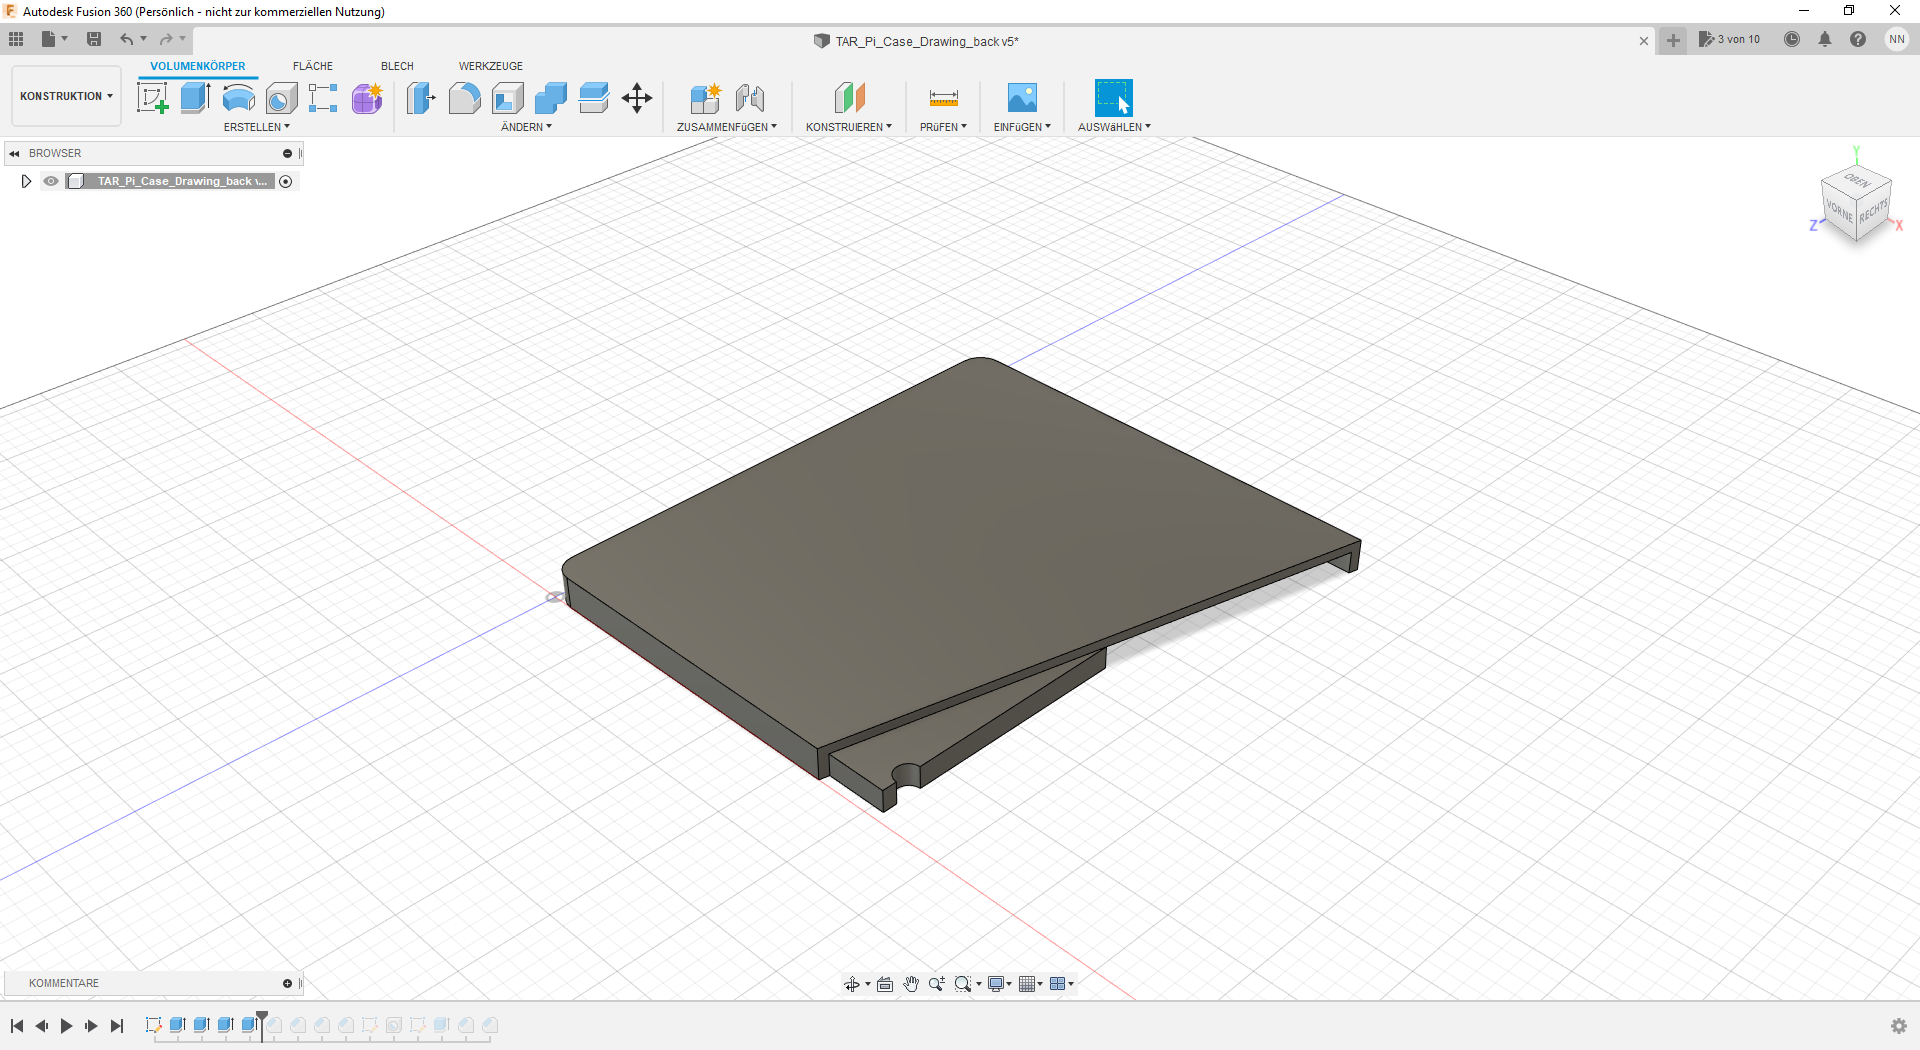
\includegraphics[width=\linewidth]{img/konstruktion_gehaeuse_hinten_005.png}
		\caption[]{}
		\label{fig:design-back-05}
	\end{subfigure}
	\begin{subfigure}[t]{.3\linewidth}
		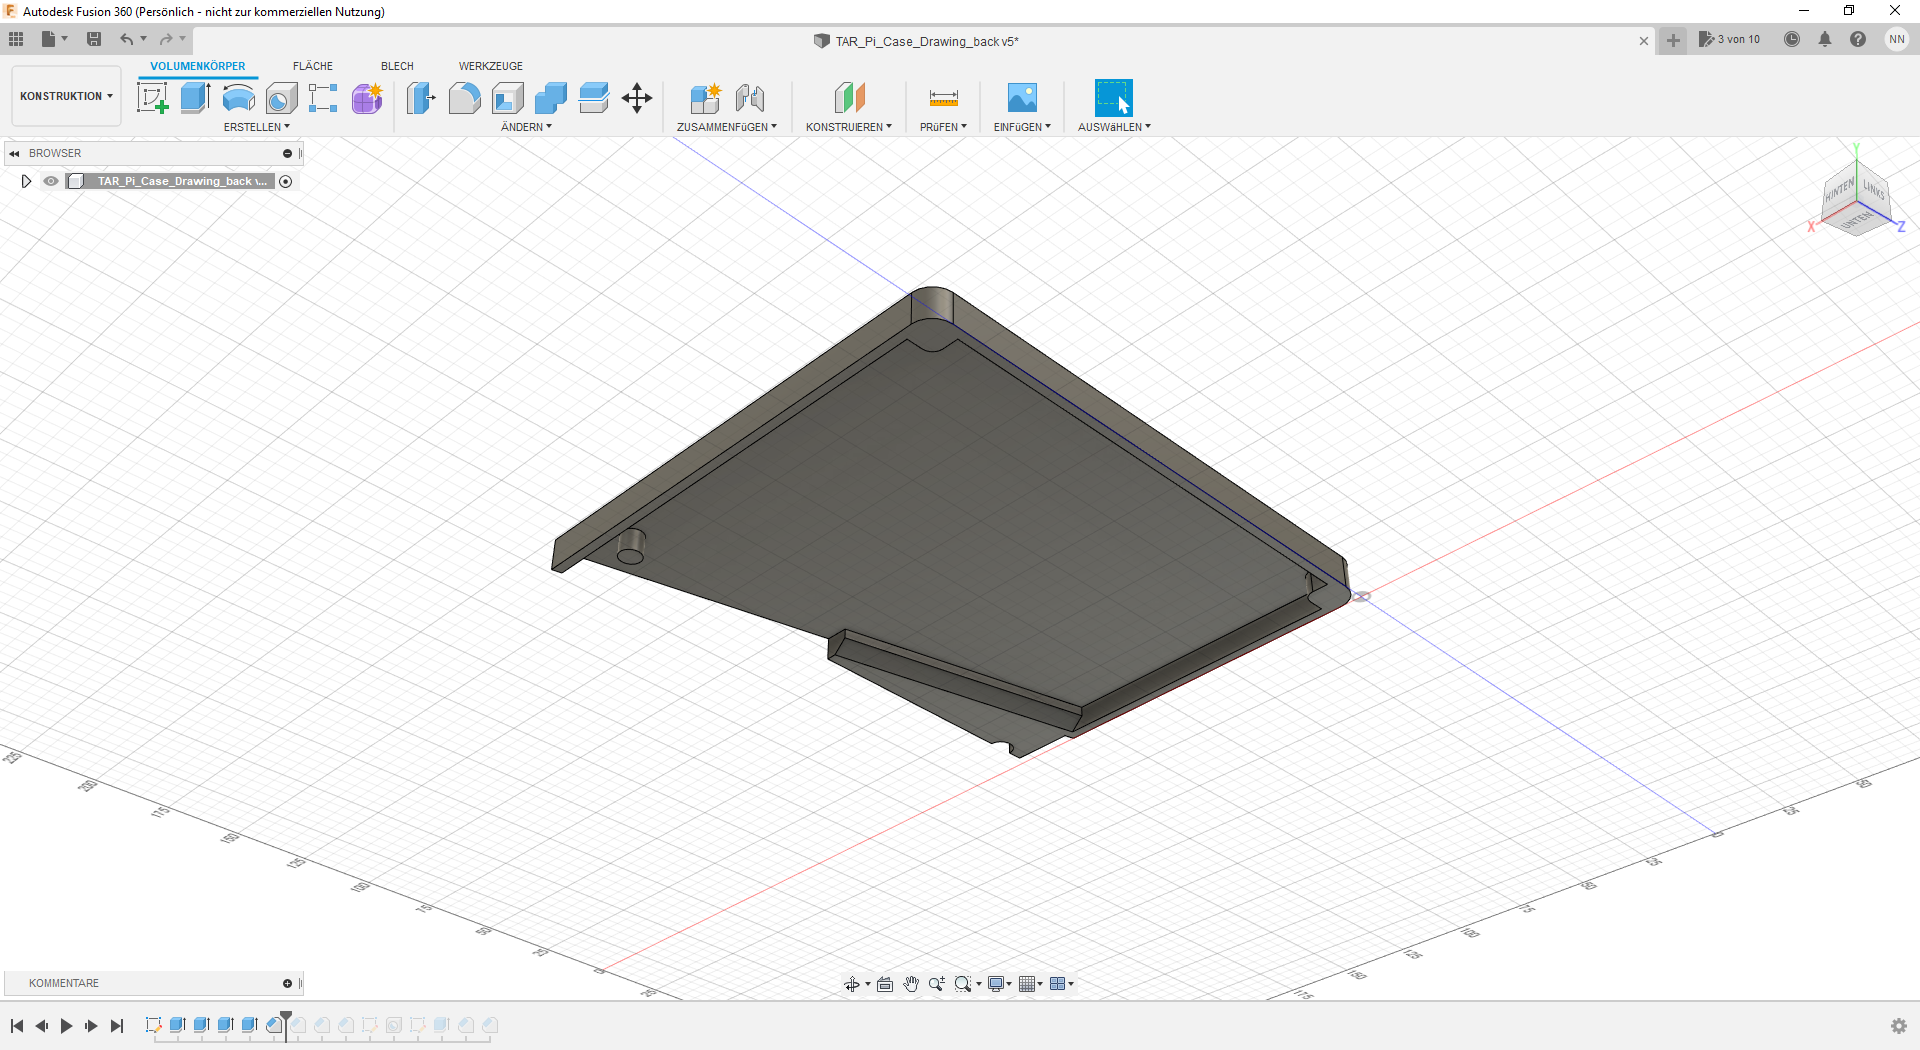
\includegraphics[width=\linewidth]{img/konstruktion_gehaeuse_hinten_006.png}
		\caption[]{}
		\label{fig:design-back-06}
	\end{subfigure}
	\begin{subfigure}[t]{.3\linewidth}
		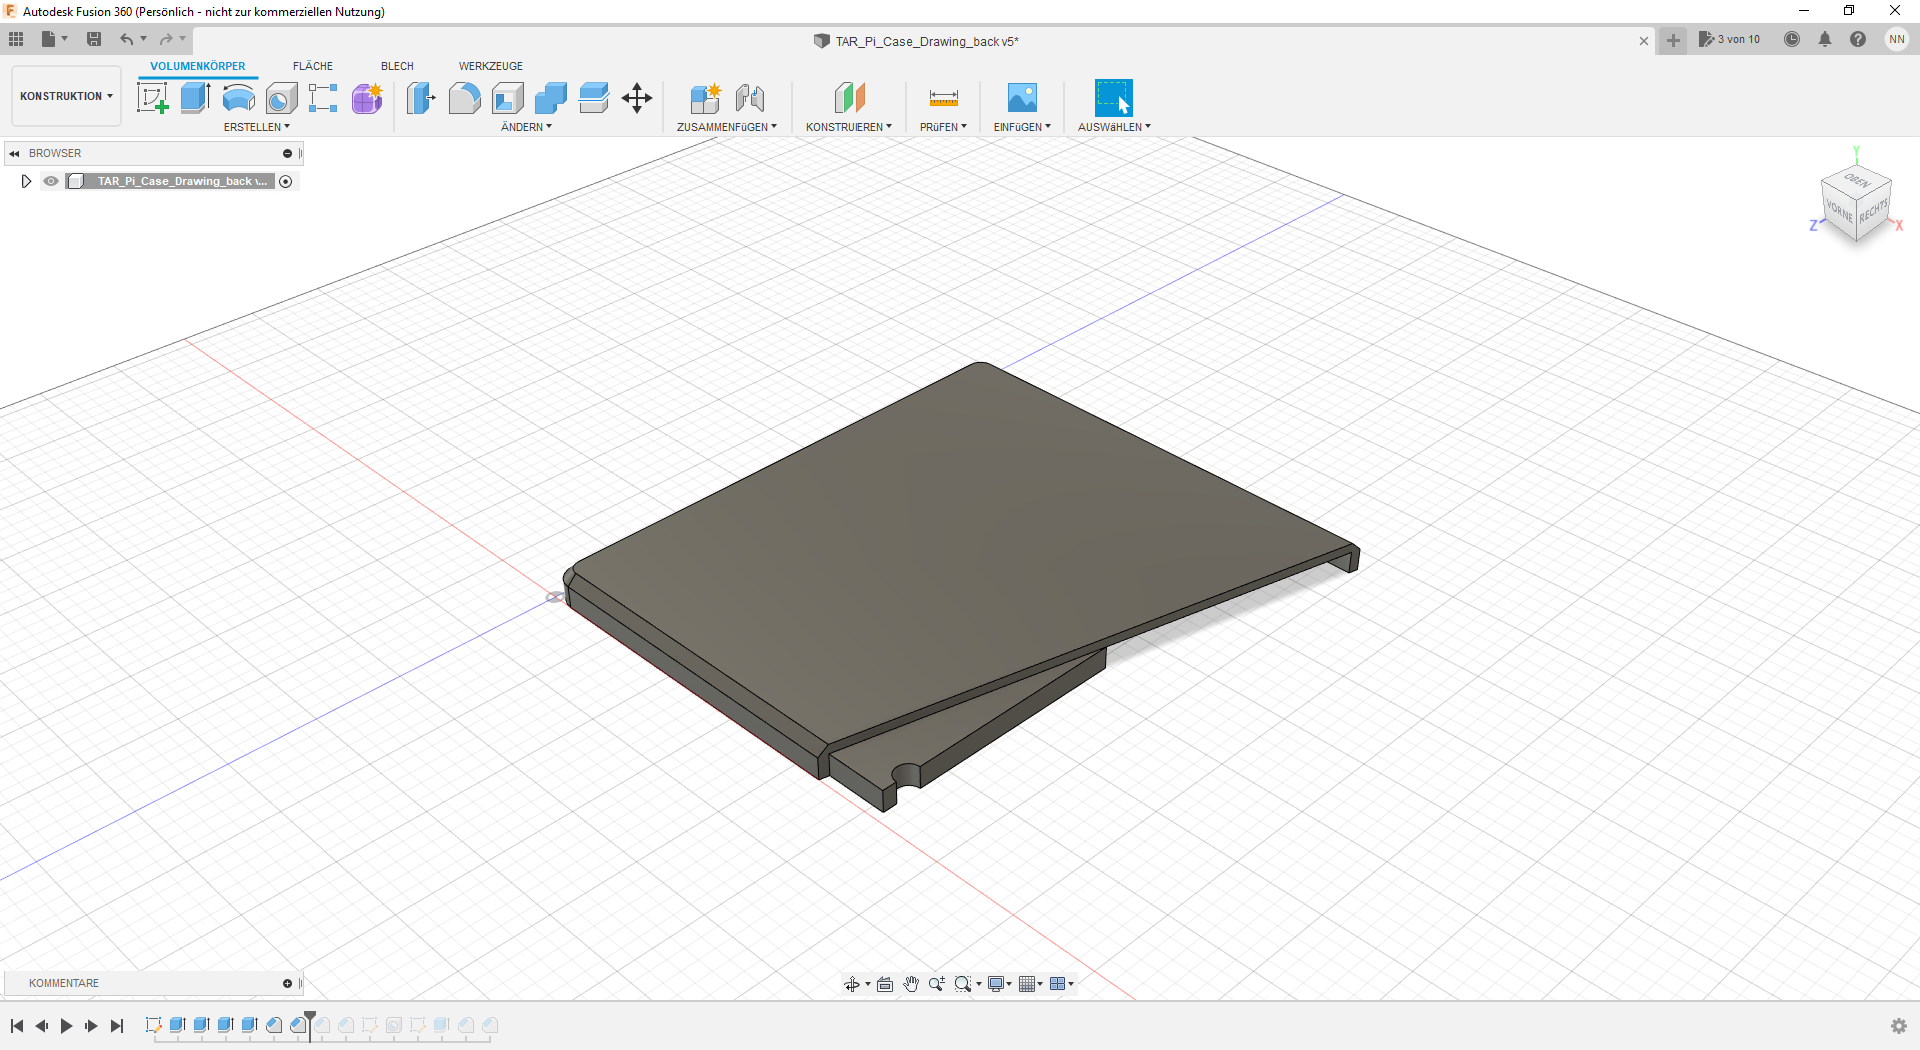
\includegraphics[width=\linewidth]{img/konstruktion_gehaeuse_hinten_007.png}
		\caption[]{}
		\label{fig:design-back-07}
	\end{subfigure}
	\begin{subfigure}[t]{.3\linewidth}
		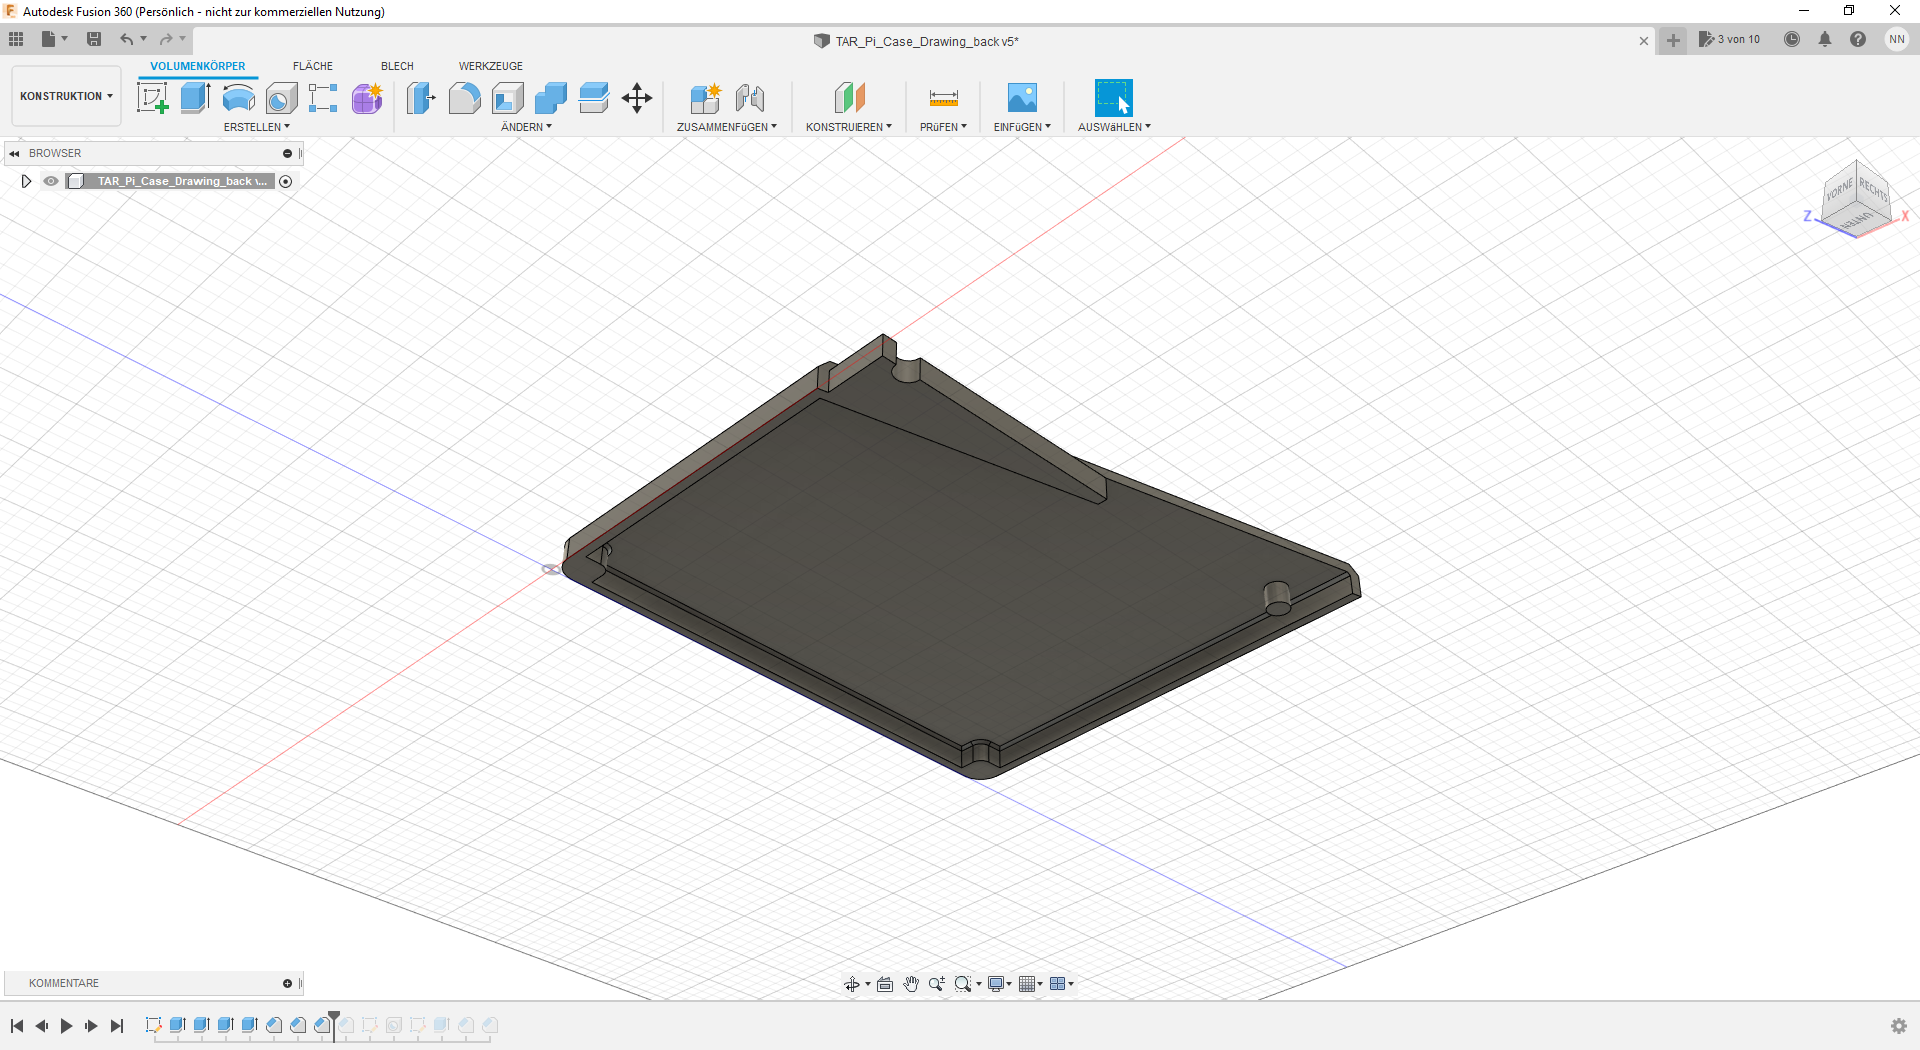
\includegraphics[width=\linewidth]{img/konstruktion_gehaeuse_hinten_008.png}
		\caption[]{}
		\label{fig:design-back-08}
	\end{subfigure}
	\begin{subfigure}[t]{.3\linewidth}
		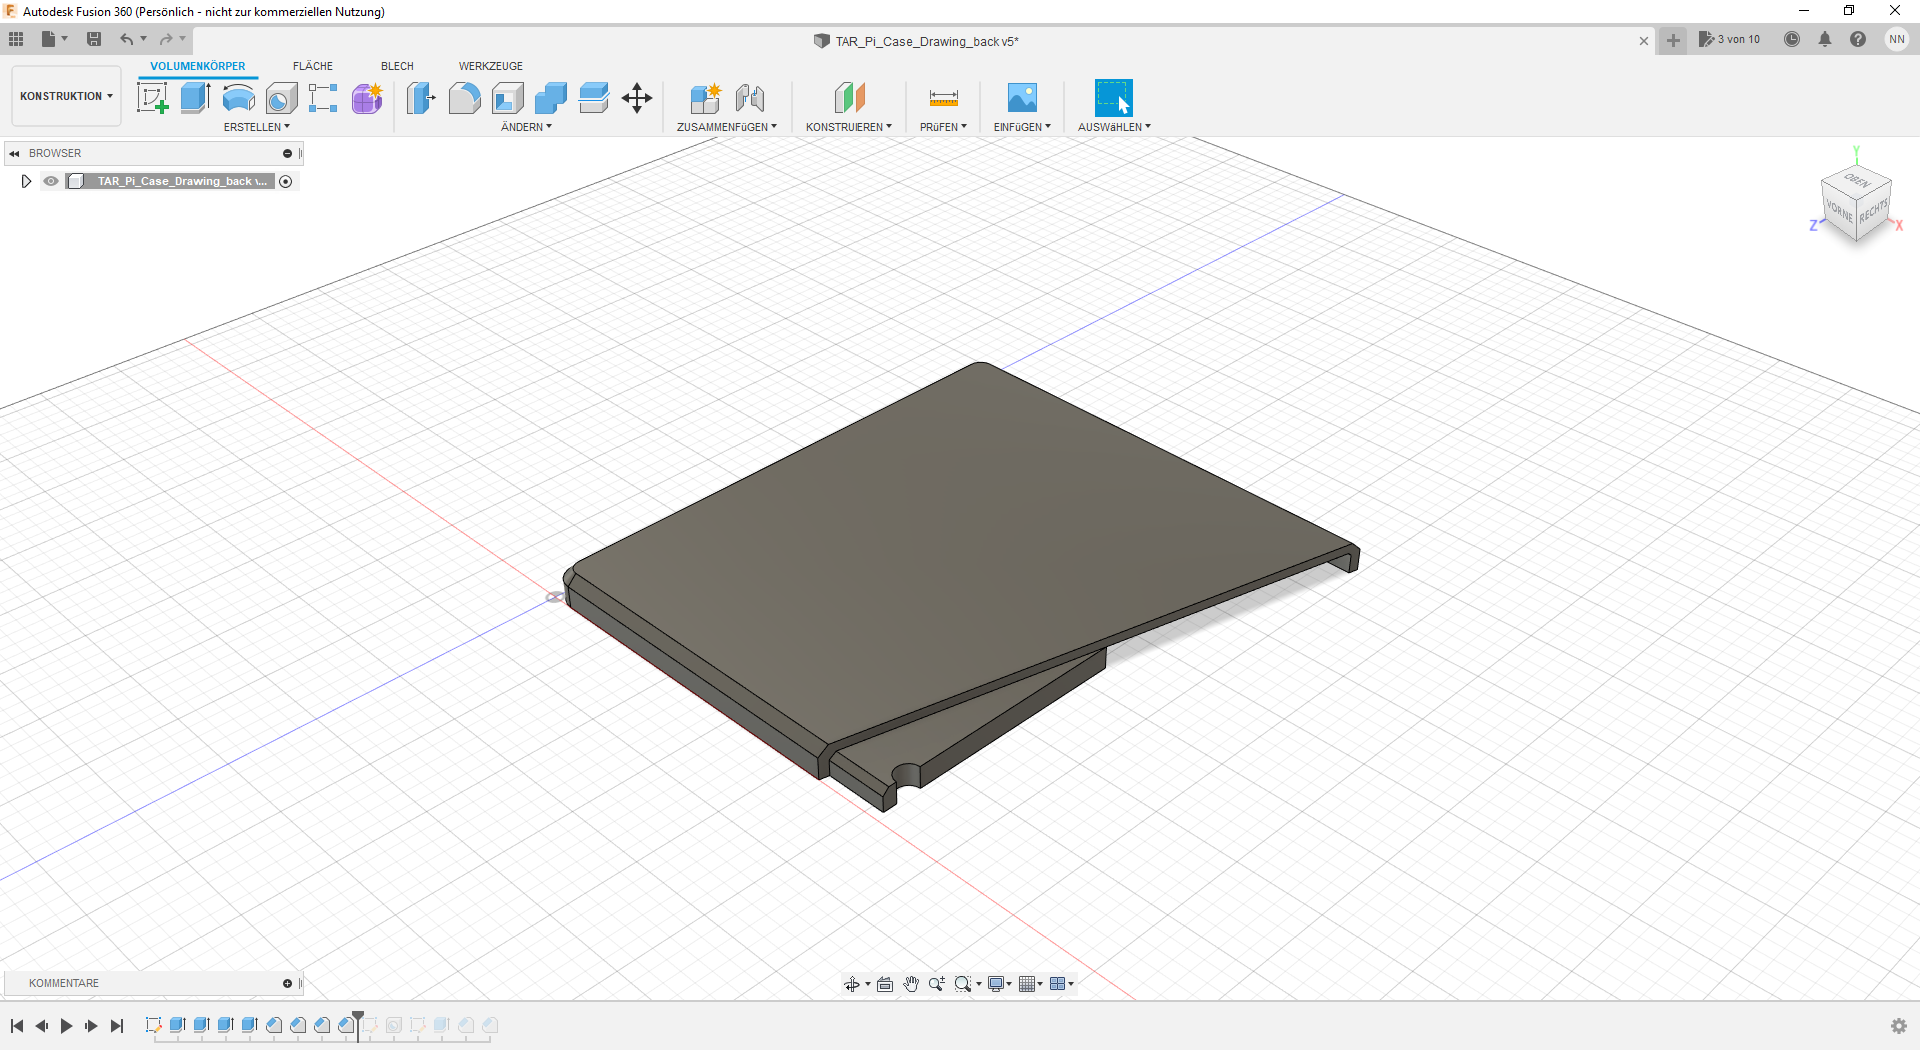
\includegraphics[width=\linewidth]{img/konstruktion_gehaeuse_hinten_009.png}
		\caption[]{}
		\label{fig:design-back-09}
	\end{subfigure}
	\begin{subfigure}[t]{.3\linewidth}
		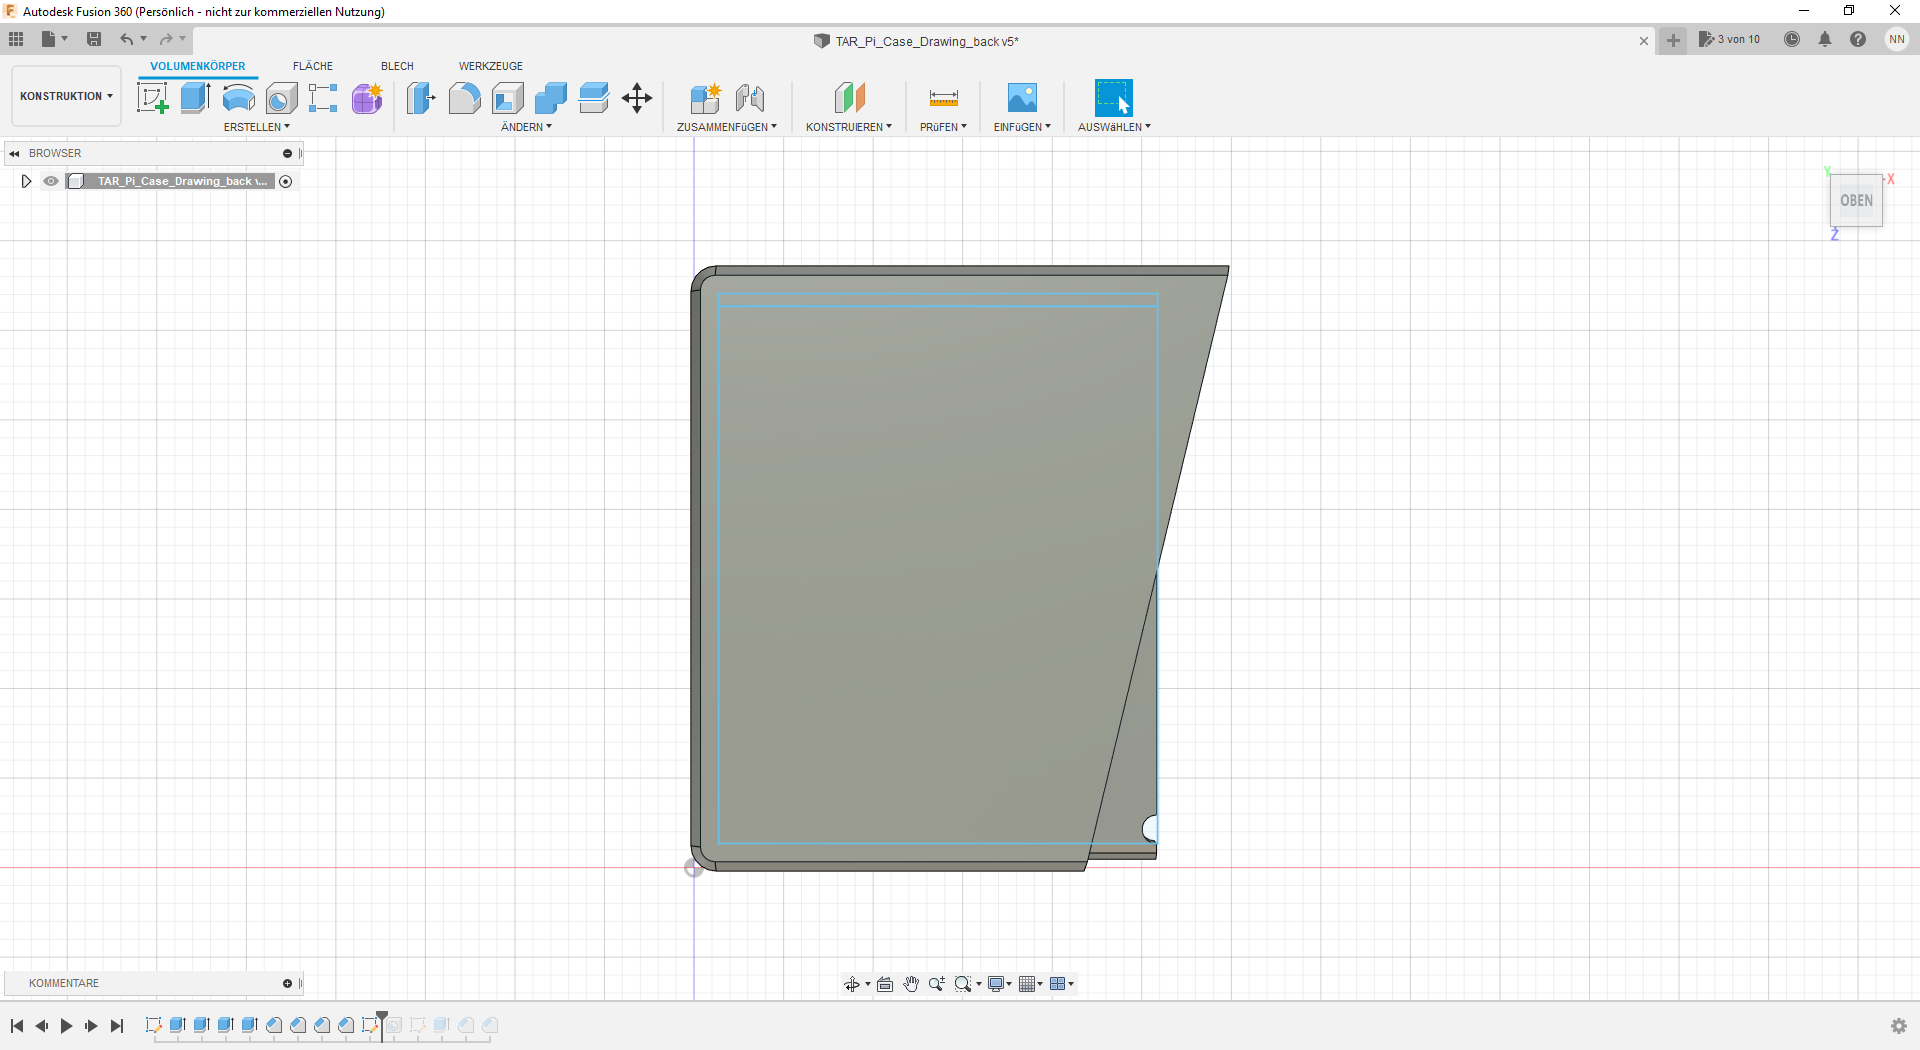
\includegraphics[width=\linewidth]{img/konstruktion_gehaeuse_hinten_010.png}
		\caption[]{}
		\label{fig:design-back-10}
	\end{subfigure}
	\begin{subfigure}[t]{.3\linewidth}
		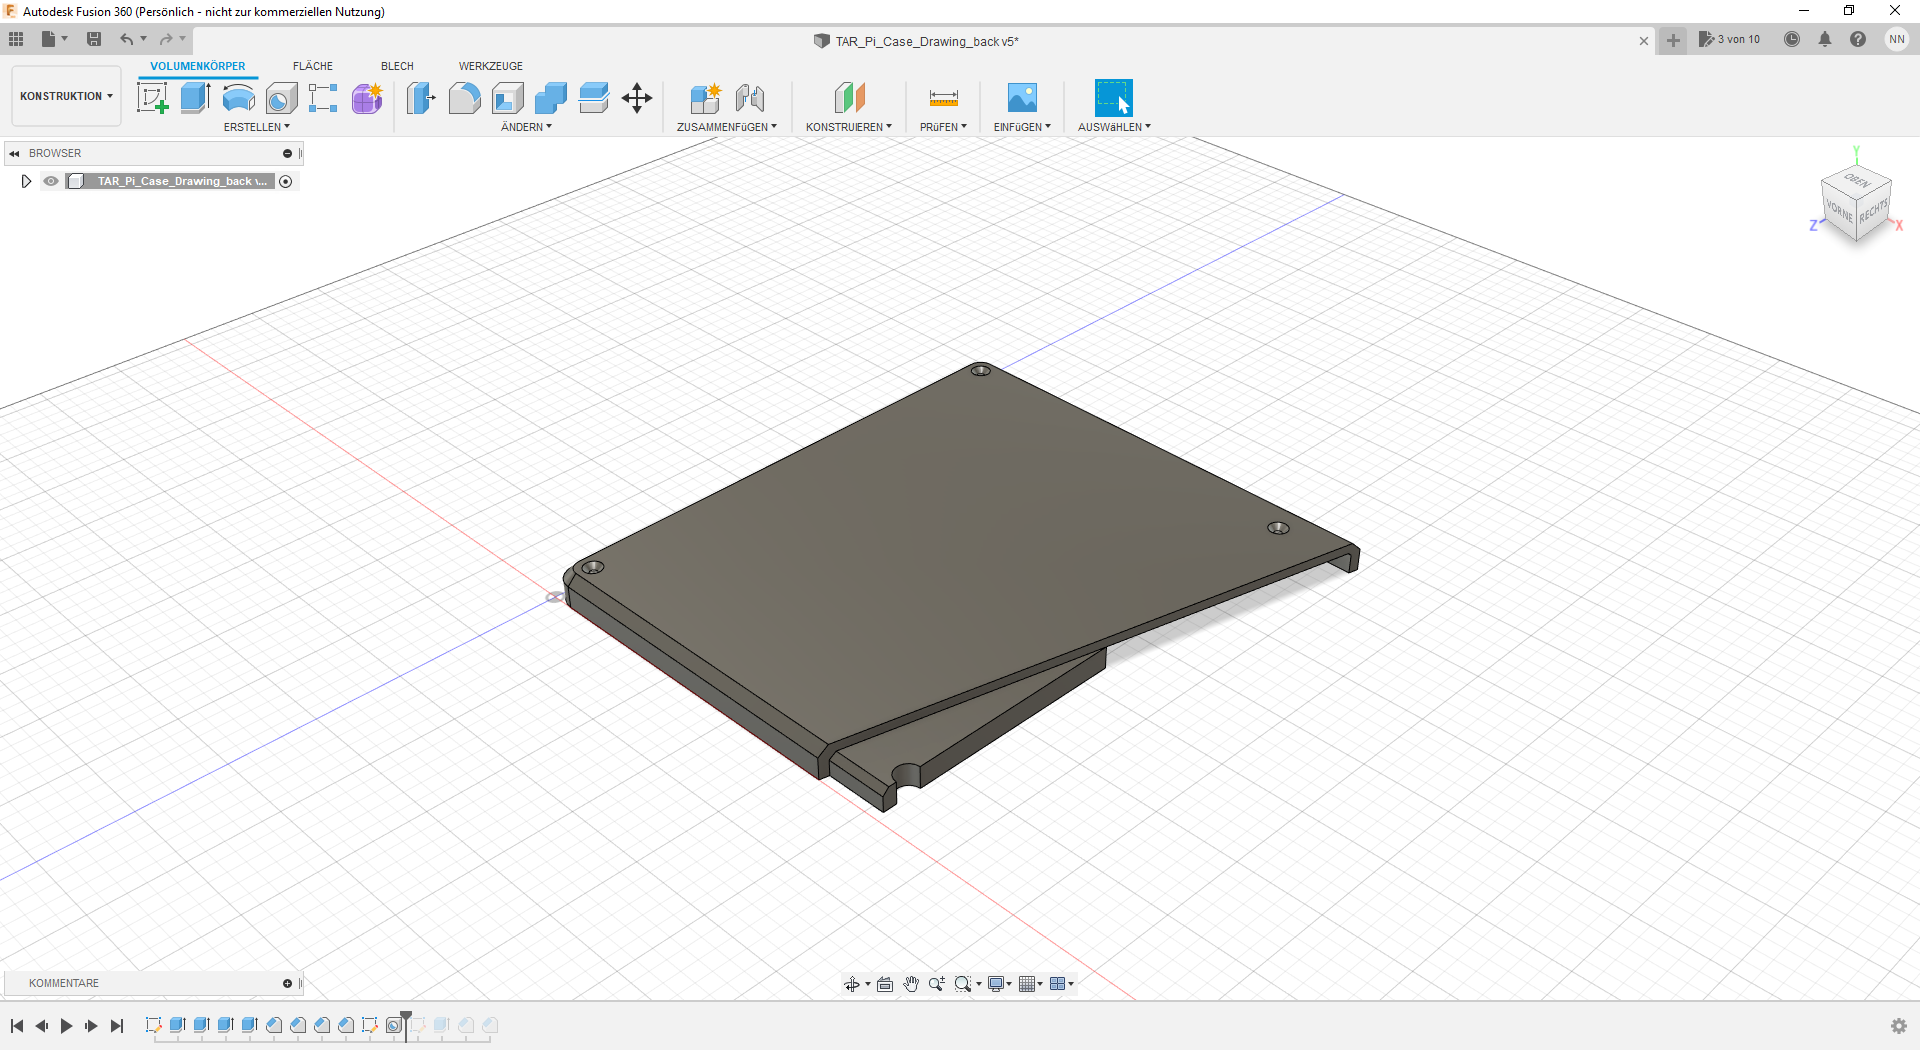
\includegraphics[width=\linewidth]{img/konstruktion_gehaeuse_hinten_011.png}
		\caption[]{}
		\label{fig:design-back-11}
	\end{subfigure}
	\begin{subfigure}[t]{.3\linewidth}
		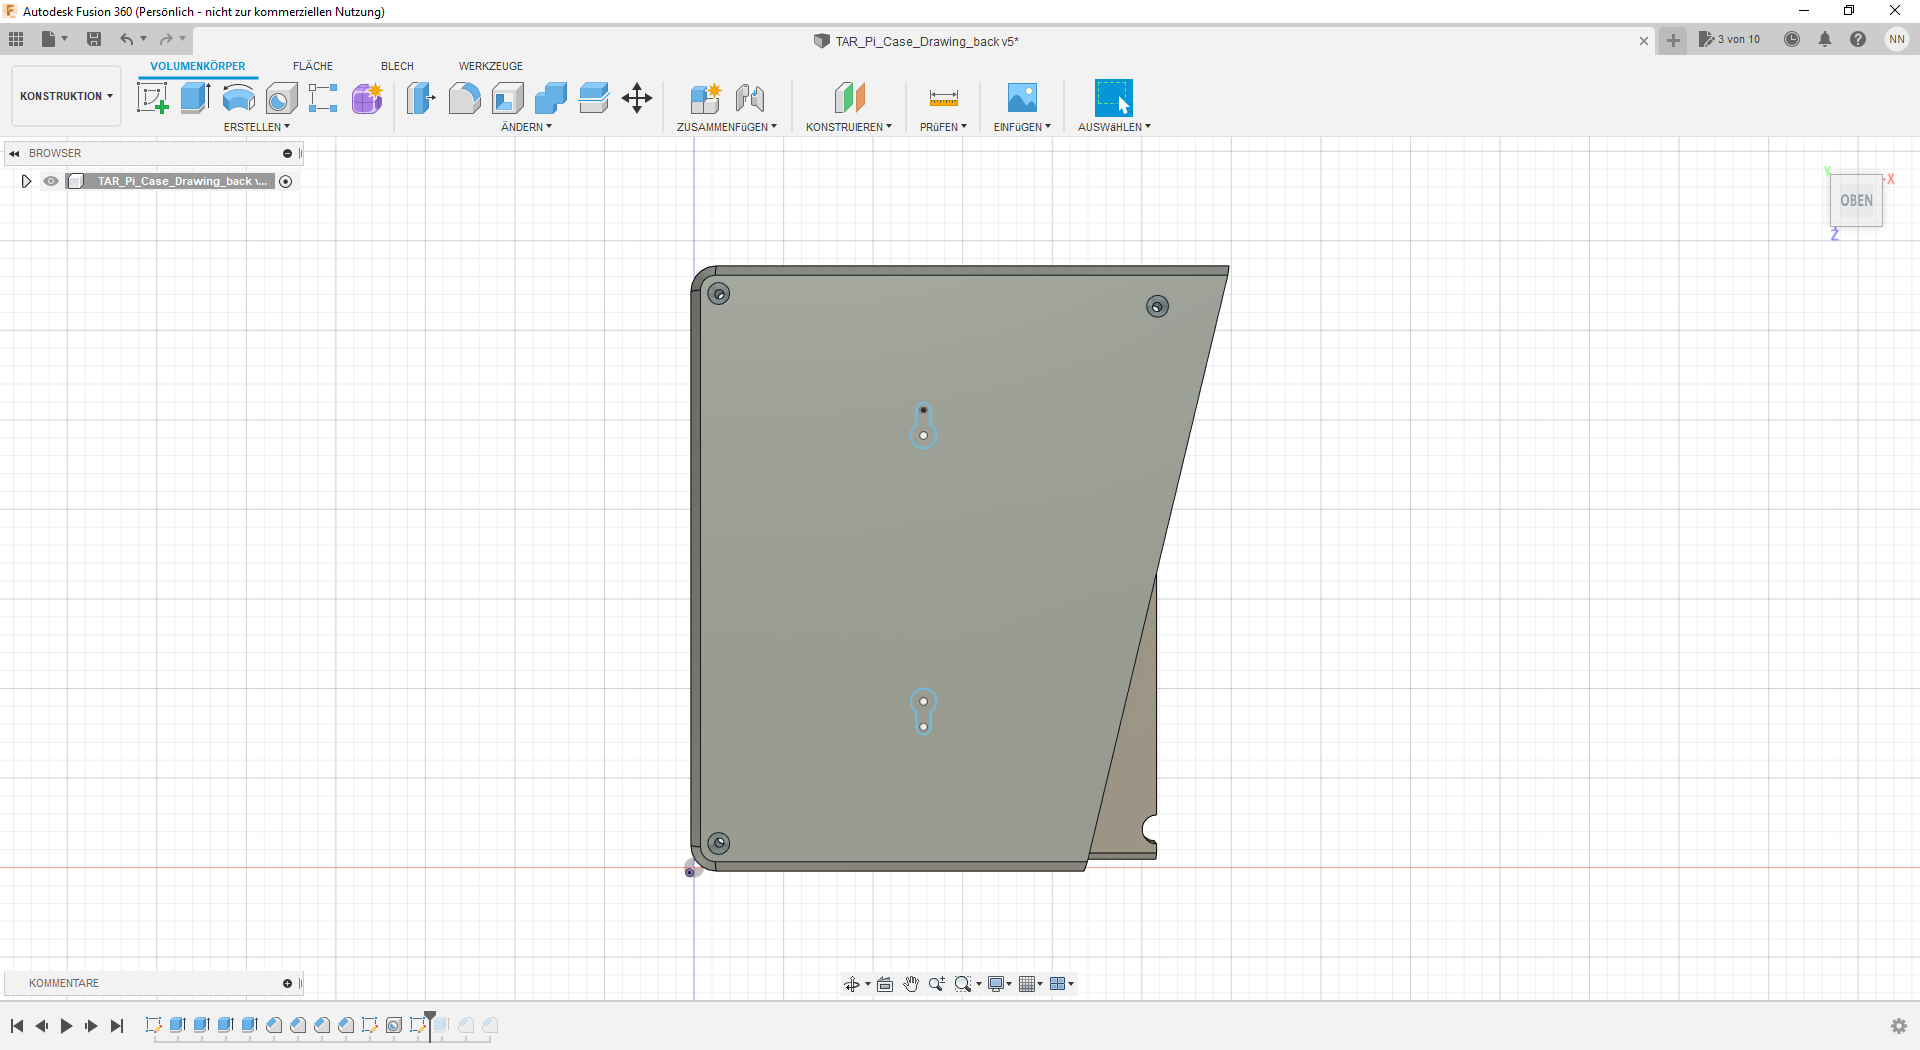
\includegraphics[width=\linewidth]{img/konstruktion_gehaeuse_hinten_012.png}
		\caption[]{}
		\label{fig:design-back-12}
	\end{subfigure}
	\begin{subfigure}[t]{.3\linewidth}
		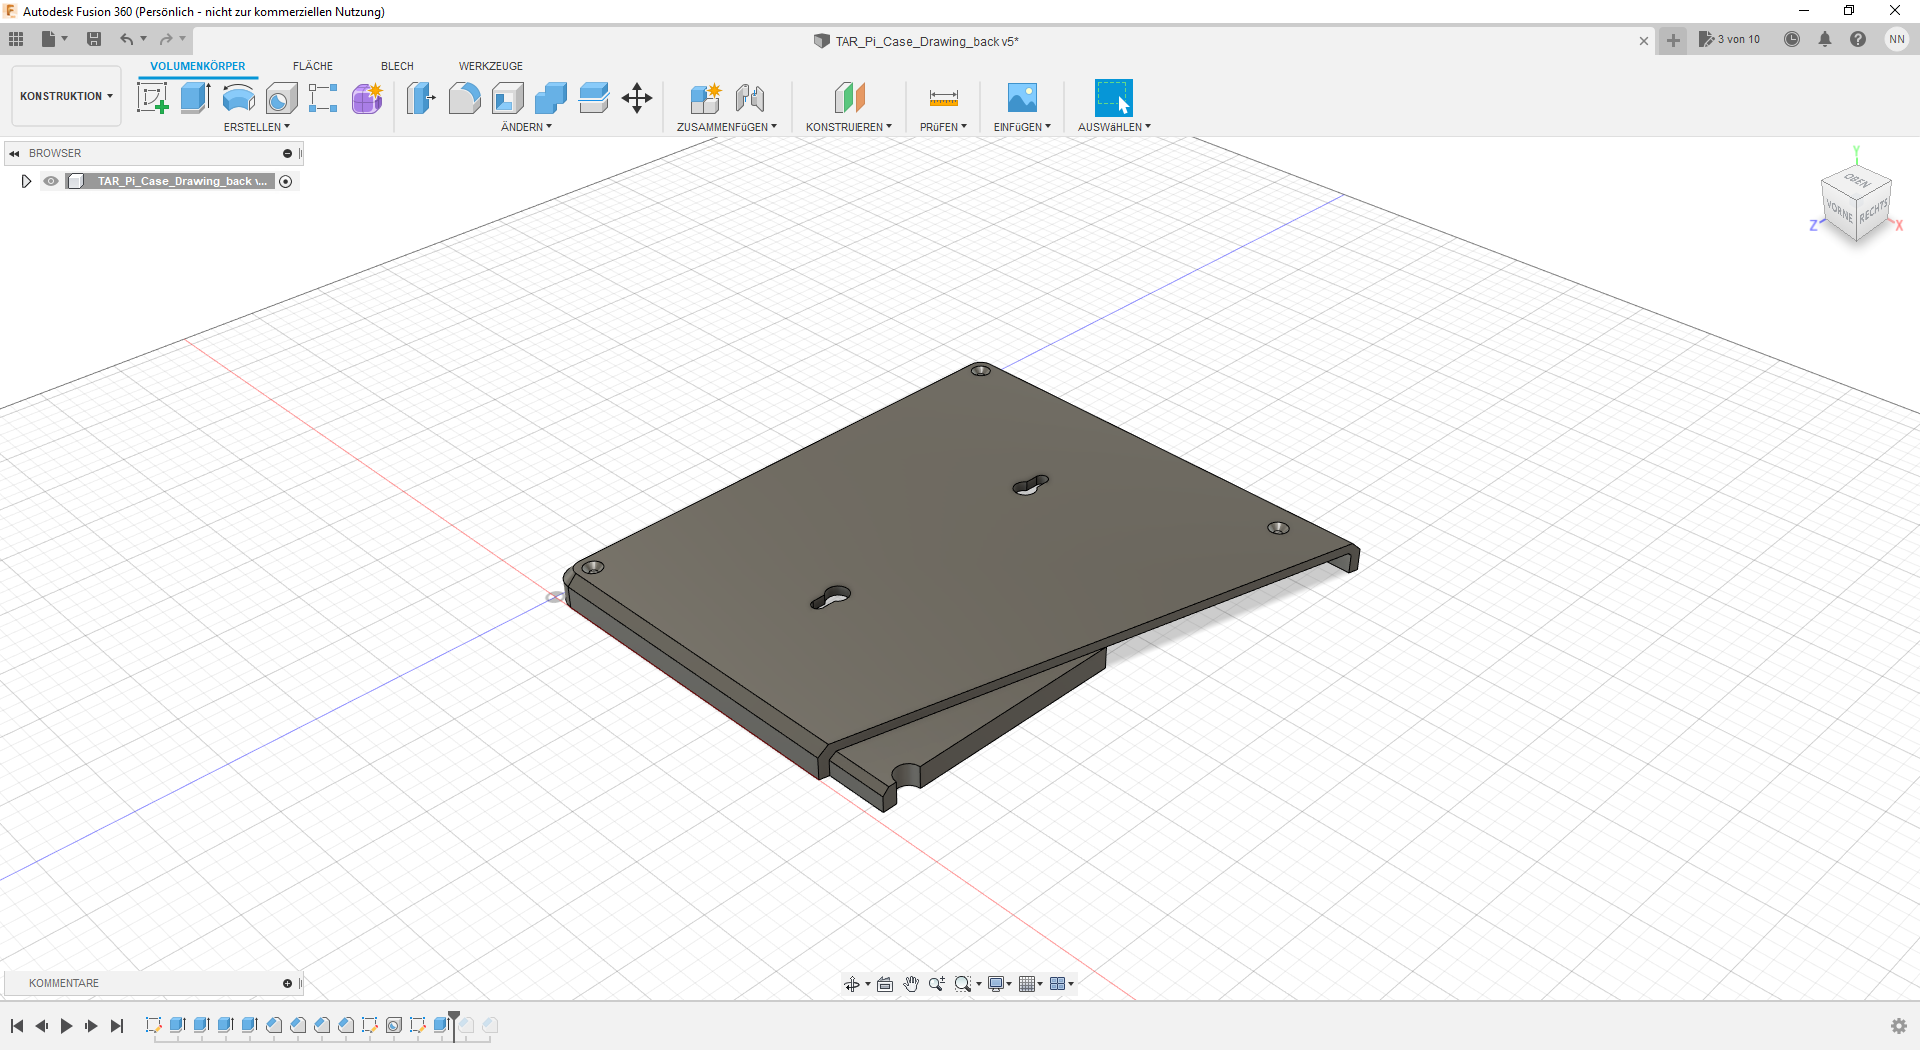
\includegraphics[width=\linewidth]{img/konstruktion_gehaeuse_hinten_013.png}
		\caption[]{}
		\label{fig:design-back-13}
	\end{subfigure}
	\begin{subfigure}[t]{.3\linewidth}
		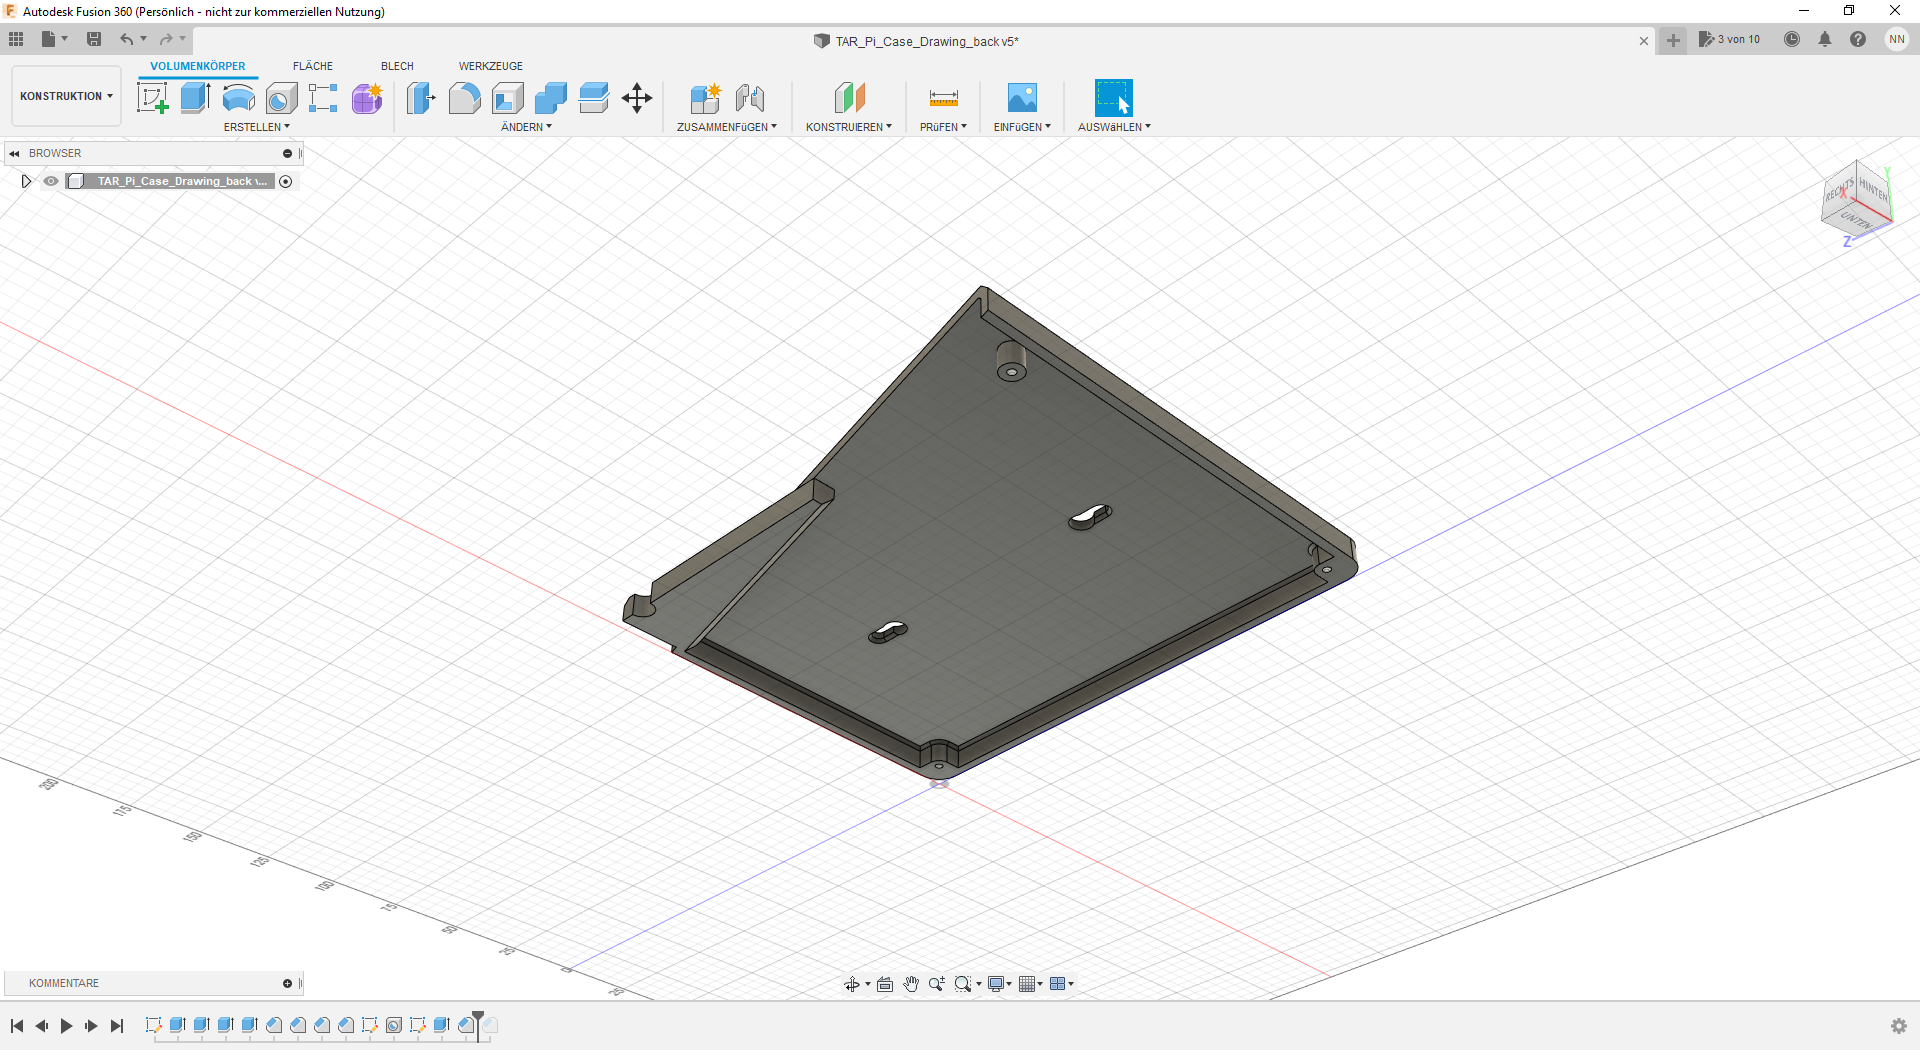
\includegraphics[width=\linewidth]{img/konstruktion_gehaeuse_hinten_014.png}
		\caption[]{}
		\label{fig:design-back-14}
	\end{subfigure}
	\begin{subfigure}[t]{.3\linewidth}
		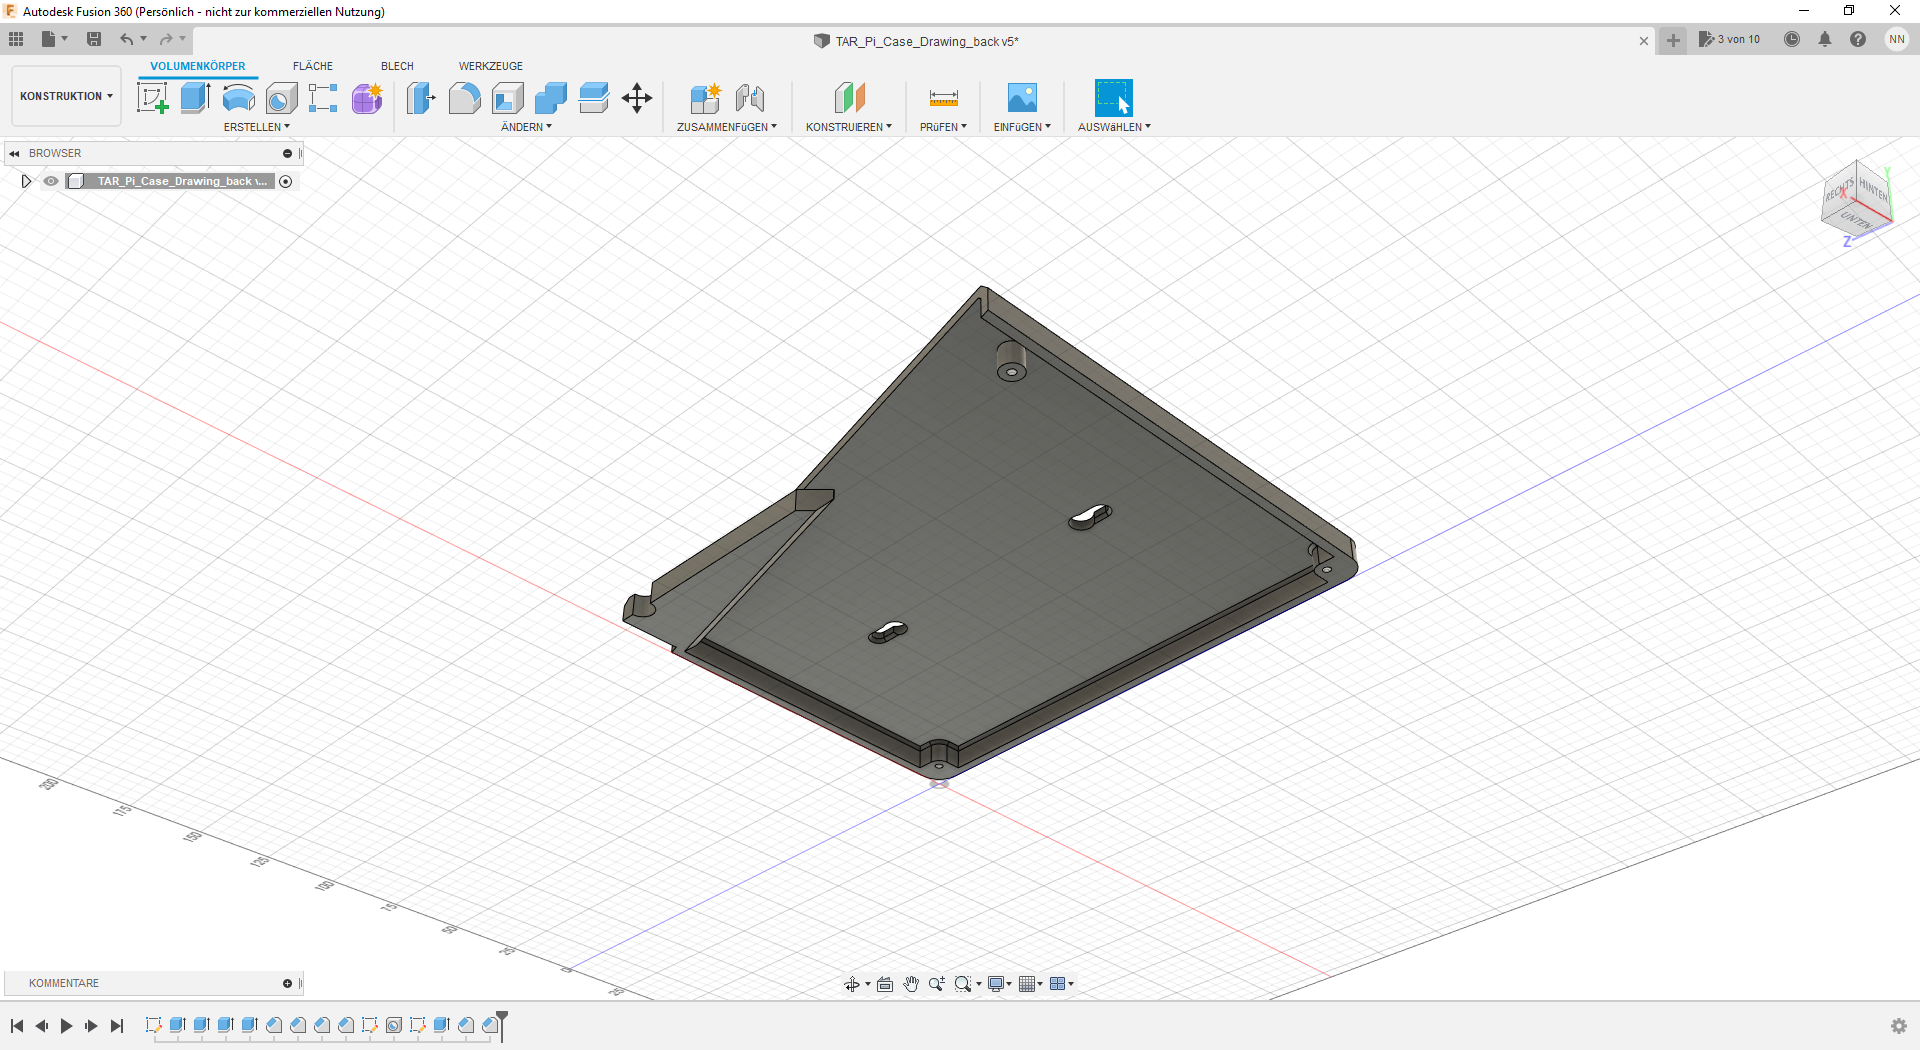
\includegraphics[width=\linewidth]{img/konstruktion_gehaeuse_hinten_015.png}
		\caption[]{}
		\label{fig:design-back-15}
	\end{subfigure}
	\caption[Entwurf der Gehäuserückwand]{Entwurf der Gehäuserückwand}
	\label{fig:design-back}
\end{figure}\par
\newpage